\chapter{Comparative Phylogenetics of PVC Operons}\label{bioinformatics}

\epigraph{\textit{``You should use more mathematics, like we do."}}{Richard P. Feynman}

\section{Introduction}
The PVCs are complex operons for which the paradoxical idiom ``the same but different" very much applies. Of the 16 operons  observed in the 3 strains most commonly studied in the lab, there few real `hard-and-fast' rules that can applied to all of them - other than that they elaborate the same ultimate structure. Just with some simple `sequence-gazing', quite drastic differences can be identified easily.

There have been quite extensive studies of analogous systems to the PVCs, such as phage (see \citep{Yap2014} for a good review), R-type pyocins/tailocins \citep{Ge2015, Ghequire2015}, and membrane bound secretion systems \citep{Cascales2012}, that can be found in the literature \citep{Sarris2014, Kube2015} (these are just illustrative examples, a more exhaustive literature search can be found in \vref{intro}). However, these types of comparison studies tend to focus on the common features between these systems, without paying much, if any, attention to what it is that makes them different (e.g. identifying them all as contractile mechanisms). Given the diversity seen among PVC elements within even the same genome, it seems clear that the Devil is in the detail, and it's actually what sets each PVC apart from one another that is of most interest, given the `effort' \Pa{} is going to, to maintain 5-6 highly paralogous sequences.

To date, there has been no real attempt to perform a systematic analysis of all of the operons, and much of what is known of the functions of genes within has been predicted from (now aged) genome annotations and simple BLAST studies `by hand'. The Sarris et al. paper attempted to do a systematic study of contractile tail structures across many genera, but at the expense of studying any of them in great detail, and again, focussed on the common details, defining a `consensus operon'. In this chapter, this is addressed within the scope of PVCs specifically, highlighting the micro-evolution that sets these operons apart from one another, and from related structures in other genera.

The micro-evolution within the operons was examined here via a phylogenetic congruency workflow. Genes within the PVC operons are compared for their sequence divergence and ability to accurately represent the known phylogenetic history of the genus. Those which are found to be incongruent are inferred to be evolving differentially. The chapter speculates, based on the clustering of PVCs with their effectors, how interchangeable PVC components may be, versus whether they are honed in some way to each of their cognate effectors. Additionally, this chapter attempts to define the hallmarks of PVCs, such that contractile tail like systems in as yet unstudied genomes can be identified, and demarcated from other contractile tail like structures.

\subsection*{Chapter Aims:}
\begin{itemize}
	\item Create a systematic, comparative analysis of genes within PVC operons.
	\item Establish the likelihood and extent of recombination within the operons.
	\item Establish a criteria/framework for identifying PVC-like elements in additional genomes.
\end{itemize}

\section{Experimental Procedures}
This section describes, at a higher level, the workflow and concepts required for the analysis conducted. Specific details of algorithmic parameters, software versions and other technical details are reserved for \vref{methods}.

\vspace{0.5cm}
\tikzstyle{decision} = [diamond, draw, fill=blue!20, text width=4.5em, text badly centered, node distance=3cm, inner sep=0pt]
\tikzstyle{block} = [rectangle, draw, fill=blue!20, text centered, rounded corners]
\tikzstyle{line} = [draw, -latex']
\tikzstyle{cloud} = [draw, ellipse,fill=red!20, node distance=3cm, minimum height=2em]
\tikzstyle{startstop} = [rectangle, rounded corners, text centered, draw=black, fill=red!30]
\tikzstyle{io} = [trapezium, trapezium left angle=70, trapezium right angle=110, text centered, draw=black, fill=green!30]
\tikzstyle{arrow} = [thick,->,>=stealth]

\begin{center}
\begin{figure}[h]
\begin{tikzpicture}[node distance = 2.2cm, auto]

    % Place nodes
    \node [align=center, font=\scriptsize\linespread{0.8}, startstop] (init) {Cluster\\ orthologues\par};
    \node [align=center, font=\scriptsize\linespread{0.8}, block, right of=init] (acquire) { Curate\\ Sequences};
    \node [align=center, font=\scriptsize\linespread{0.8}, block, right of=acquire] (msa) { Multiple\\ Sequence\\ Alignment};
    \node [align=center, font=\scriptsize\linespread{0.8}, yshift=0.3cm, io, below left=0.7cm and -0.2cm of msa] (GC) {GC};
    \node [align=center, font=\scriptsize\linespread{0.8}, yshift=0.3cm, io, below right=0.7cm and -0.2cm of msa] (ID) {AA\%ID};
    \node [align=center, font=\scriptsize\linespread{0.8}, block, right of=msa] (gtrees) {Create\\ gene trees};
    \node [align=center, font=\scriptsize\linespread{0.8}, block, right of=gtrees] (stree) {Infer\\ Consensus tree};
    \node [align=center, font=\scriptsize\linespread{0.8}, block, right of=stree] (congruency) {Calculate\\ congruency};
    \node [align=center, font=\scriptsize\linespread{0.8}, startstop, right of=congruency] (viz) {Visualise\\ results};



    % Draw Edges
    \path [line] (init) -- (acquire);
    \path [line] (acquire) -- (msa);
    \path [line] (msa) -- (gtrees);
    \path [line, dashed] (msa) -- (GC);
    \path [line, dashed] (msa) -- (ID);
    \path [line] (gtrees) -- (stree);
    \path [line] (stree) -- (congruency);
    \coordinate (Above gtrees) at ($(gtrees.north)+(0,0.5cm)$);
    \coordinate (Above congruency) at ($(congruency.north)+(0,0.5cm)$);
    \path [line] (gtrees.north) -- (Above gtrees) -- (Above congruency) -- (congruency.north);
    \path [line] (congruency) -- (viz);

%    \path [line,dashed] (expert) -- (init);
%    \path [line,dashed] (system) -- (init);
%    \path [line,dashed] (system) |- (evaluate);

\end{tikzpicture}
\captionsetup{singlelinecheck=off, justification=justified, font=footnotesize, aboveskip=15pt}
\caption[Congruency workflow flowchart]{A flowchart to demonstrate, at high level, the steps involved in the process of the congruency analysis presented in this chapter.}

\end{figure}
\end{center}

\subsection{Syntenic Clustering of Orthologs}\label{clustering}
In order to analyse each gene, they had to be separated out in to syntenic clusters. Since we elected to use 16 operons, totalling around 300 genes, the list was curated manually. This was preferable in this instance versus a computational approach (e.g. syntenic clustering with programs), due to the differences between operons where genes may be missing or unique, which complicates the process. It was also not possible to classify the sequences on sequence alone, as several of the genes within a PVC operon are direct paralogs of one another, and would thus be combined in to the same cluster if done by sequence alone, resulting in the comparison of locus 1 and locus 5 for example. \vref{orthologs} shows the clustering and nomenclature arrived at which remained consistent for the duration of the analyses. In the cases where a gene appeared to have been deleted/lost, the functional predictions from \vref{structbioinfo}, sequence similarity, locus length, and synteny with the neighbouring genes was examined. If the loss looked to be a legitimate deletion (i.e. neighbouring genes obviously belonged in other clusters), it was marked down as absent - the analysis was set up in such a way as for this not to matter however.

Additionally, for congruency analysis on a gene-by-gene basis, only the first 16 genes of the operon are used (hereafter, PVC1 to PVC16). There were a number of reasons for this. Firstly, in each PVC, there are toxin genes in the region downstream of PVC16, but there aren't always the same number, and each toxin can be completely different (they are comparatively well characterised and can be seen to be non-orthologous). Being unrelated, their alignments and resulting trees would most likely be spurious, and the resulting trees would have as few as 2 members, which is obviously not possible.

Moreover, the fact that each of the toxin genes is known to be different between each PVC (to the extent that they are used to differentiate between operons), means that the question of whether this region of the operon is recombinant seems to be answered from the outset. Secondly, between PVC16 and the toxin genes is an extremely variable region. The additional information used for classifying genes earlier in the operon is lacking for genes in the PVC16+ region, thus it was not possible to sufficiently well disentangle this region of the operon, as the genes have no known functions and no ontological information in existing databases due to their lack of similarity to anything currently known.
Many of these genes are unique, with no analogous genes. The workflow described here is tolerant to the deletion of members of a group, as long as there are other members within the group to compare with (a deletion is penalised as an incongruency). It was decided it would make for a simpler and more robust analysis to disregard these genes. 

\subsubsection{Curation of the Anomalous Lumt operon}\label{anomalouslumt}
Curation of orthologs for the Lumt operon proved to be more complicated, as the operon architecture is more distinctive; it has lost a couple of genes (one more so in ATCC43949 than in Kingscliff) and gained several others. Lumt was curated last, once all the other operons were clustered effectively. Because of this a few additional CDSs were discarded from the operon for this analysis. Firstly, there is an additional 5' preceding gene, referred to as PVC0 (refer to \vref{structbioinfo}, which belongs only to those operons. It is unclear as yet what, if any, role this protein has. Recent structural similarity searching explored in \vref{structbioinfo} has found high confidence hits, but without any clear indication of its involvement in the PVC structure/function. With no equivalent orthologs, it cannot be included in this workflow.

Both Lumt operons harbour an additional paralogue of PVC11, which appears to be similar to the gp6 phage baseplate - one of these paralogues for each Lumt operon was retained as the representative for locus 11. Additionally the Lumt operon has several genes toward the 3' end which do not match well to clusters in any of the other operons, have no well defined functions/orthologies, and throw out the numbering scheme commonly used for all the other operons. Specifically, in orthologous pairs: PAU02194 \& PAK02000, PAU02193 \& PAK01999, and PAU02192 \& PAK01998. Each of these genes are present with their counterpart in the Lumt operons from the USA and Kingscliff strains (respectively), but with no equivalent representative in any of the other PVCs.


\subsection{Curation of Sequences}
	There is legacy sequencing data published in NCBI for the 3 strains used for this analysis, \emph{Photorhabdus luminescens} TT01, \emph{P. asymbiotica} ATCC43949 (referred to here also as ``USA''), and \emph{P. asymbiotica} Kingscliff. These strains were used as they harbour the originally discovered PVC sequences as published by Yang \emph{et al.}\citep{Yang2006}, they are used routinely in the lab for experimental work, and most is known about them. Re-annotated sequences were used as mentioned in \vref{annotation}, and any locus tags referred to in this thesis are from the new annotations. There was some slight variation in the re-annotated operons, particularly in the prediction of fewer CDS features within a couple of the PVCs. The features predicted only in the older annotations were likely to be spurious as they were short, lacked similarity to known sequences when BLAST-ed, and were not always identified in all operons. Each CDS feature was extracted as a nucleotide fasta and organised in clusters according to \vref{orthologs}. 
	
As a further note on the existing confusing nomenclature; 2 operons were renamed in this study for clarity. Specifically, the PVC operons with the naming system ``Unit \#" were named as such when discovered, due to their syntenic arrangement within the genome of \emph{P. luminescens}, where 4 PVC cassettes are positioned in tandem, one after another directly (this arrangement is not present in \emph{P. asymbiotica} genomes). When the equivalent PVC was discovered in the \emph{P. asymbiotica} genomes, they were not given consistent names (instead being given the ``Unit 1" designation, indicating the first of its type found in that genome). In this study they are renamed based on their homology to the \emph{P. luminescens} counterparts. To state it plainly:

\begin{itemize}
	\item ``PVC Unit 1" in \Pa{} ATCC43949, is most similar to ``Unit 4" in \emph{P. luminescens}, and was thus renumbered to be consistent with \emph{P. luminescens} - ``PAU\_U4''
	\item ``PVC Unit  1" in \Pa{} Kingscliff, is most similar to ``Unit 2" in \emph{P. luminescens}, and was thus renumbered to be consistent with \emph{P. luminescens} - ``PAK\_U2"
\end{itemize}

\subsection{Sequence Alignment and Phylogenies}
	Nucleotide sequences for each CDS cluster were multiply aligned with Clustal Omega (ClustalO) \citep{Sievers2011} and bootstrapped trees calculated with RAxML \citep{Stamatakis2014}. \vrefrange{pvc1tree}{pvc16tree} show the resultant phylogenies obtained. All the trees are shown midpoint rooted, with nodes displayed in descending order for consistency and clarity, the trees themselves are unrooted. The equivalent amino acid alignments are given in the supplementary Appendix \vref{bioinformatics_appendix} for visualisation.

\subsubsection{GC Content and CDS Identity Within Operons}
With the sequences curated for each PVC locus and alignments produced, basic sequence statistics such as GC content and identity for each position were also gathered, for reference. 

\newpage
\begin{figure}[h!]
	\centering
	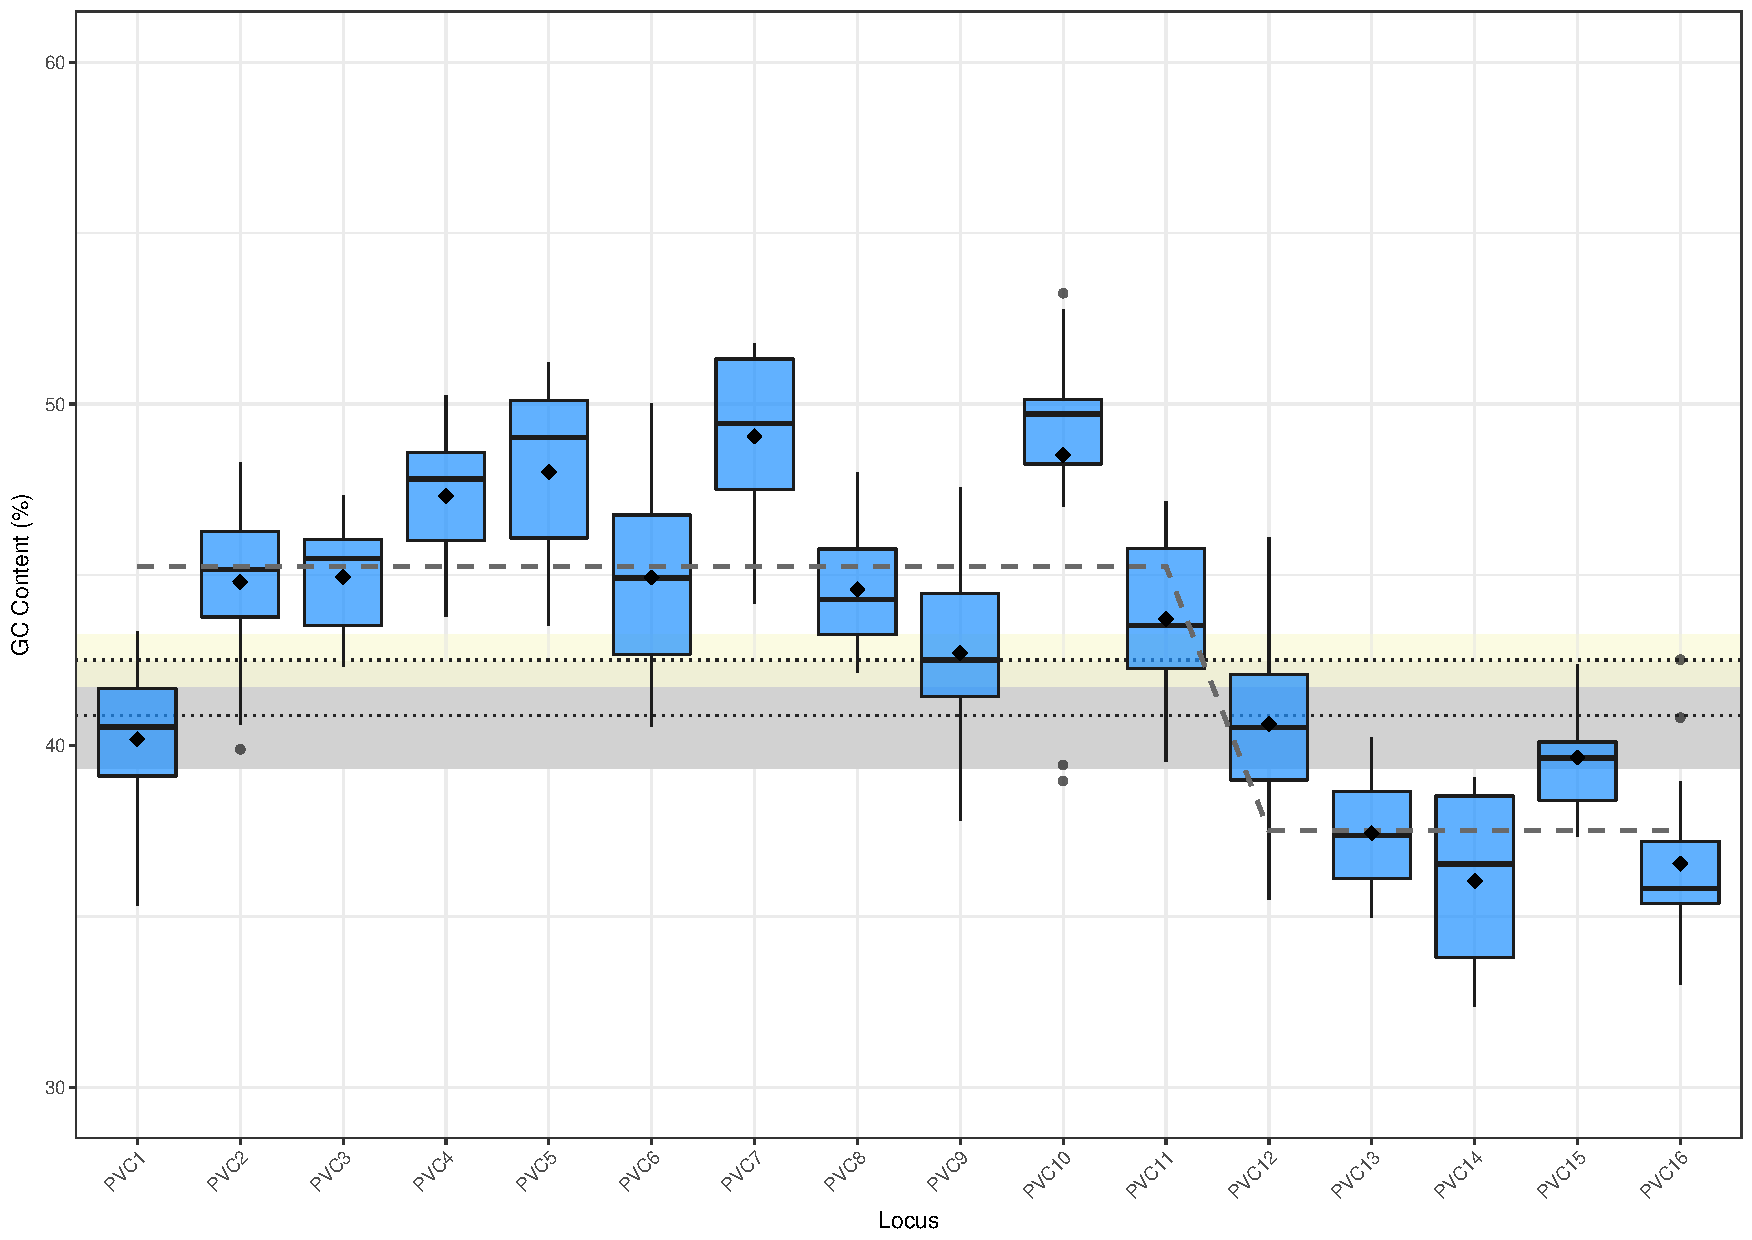
\includegraphics[width=0.8\textwidth, trim={0, 0, 0, 0}, clip]{/Users/joehealey/Documents/Warwick/PhD/Thesis/chapters/chapter4/img/GC_boxplot_with_means.pdf}
	\captionsetup{singlelinecheck=off, justification=justified, font=footnotesize, aboveskip=10pt}
	\caption[GC Content of PVC Genes]{\textsc{\normalsize The GC content (\%) distribution of PVC loci.}\vspace{0.1cm} \newline There is a trend toward significantly lower GC content at the 3' end of the operon. $\blacklozenge$ denotes the mean, $\bullet$ denotes extreme outliers outside 1.5$\times$ the interquartile range for the sample, and the black line is the median. The beige box surrounding the upper dotted line shows the mean and standard deviation of the genome GC content. The grey box and lower dotted line depict the same information, but for just the operons.}
	\label{GC}
\end{figure}

\begin{figure}[h!]
	\centering
	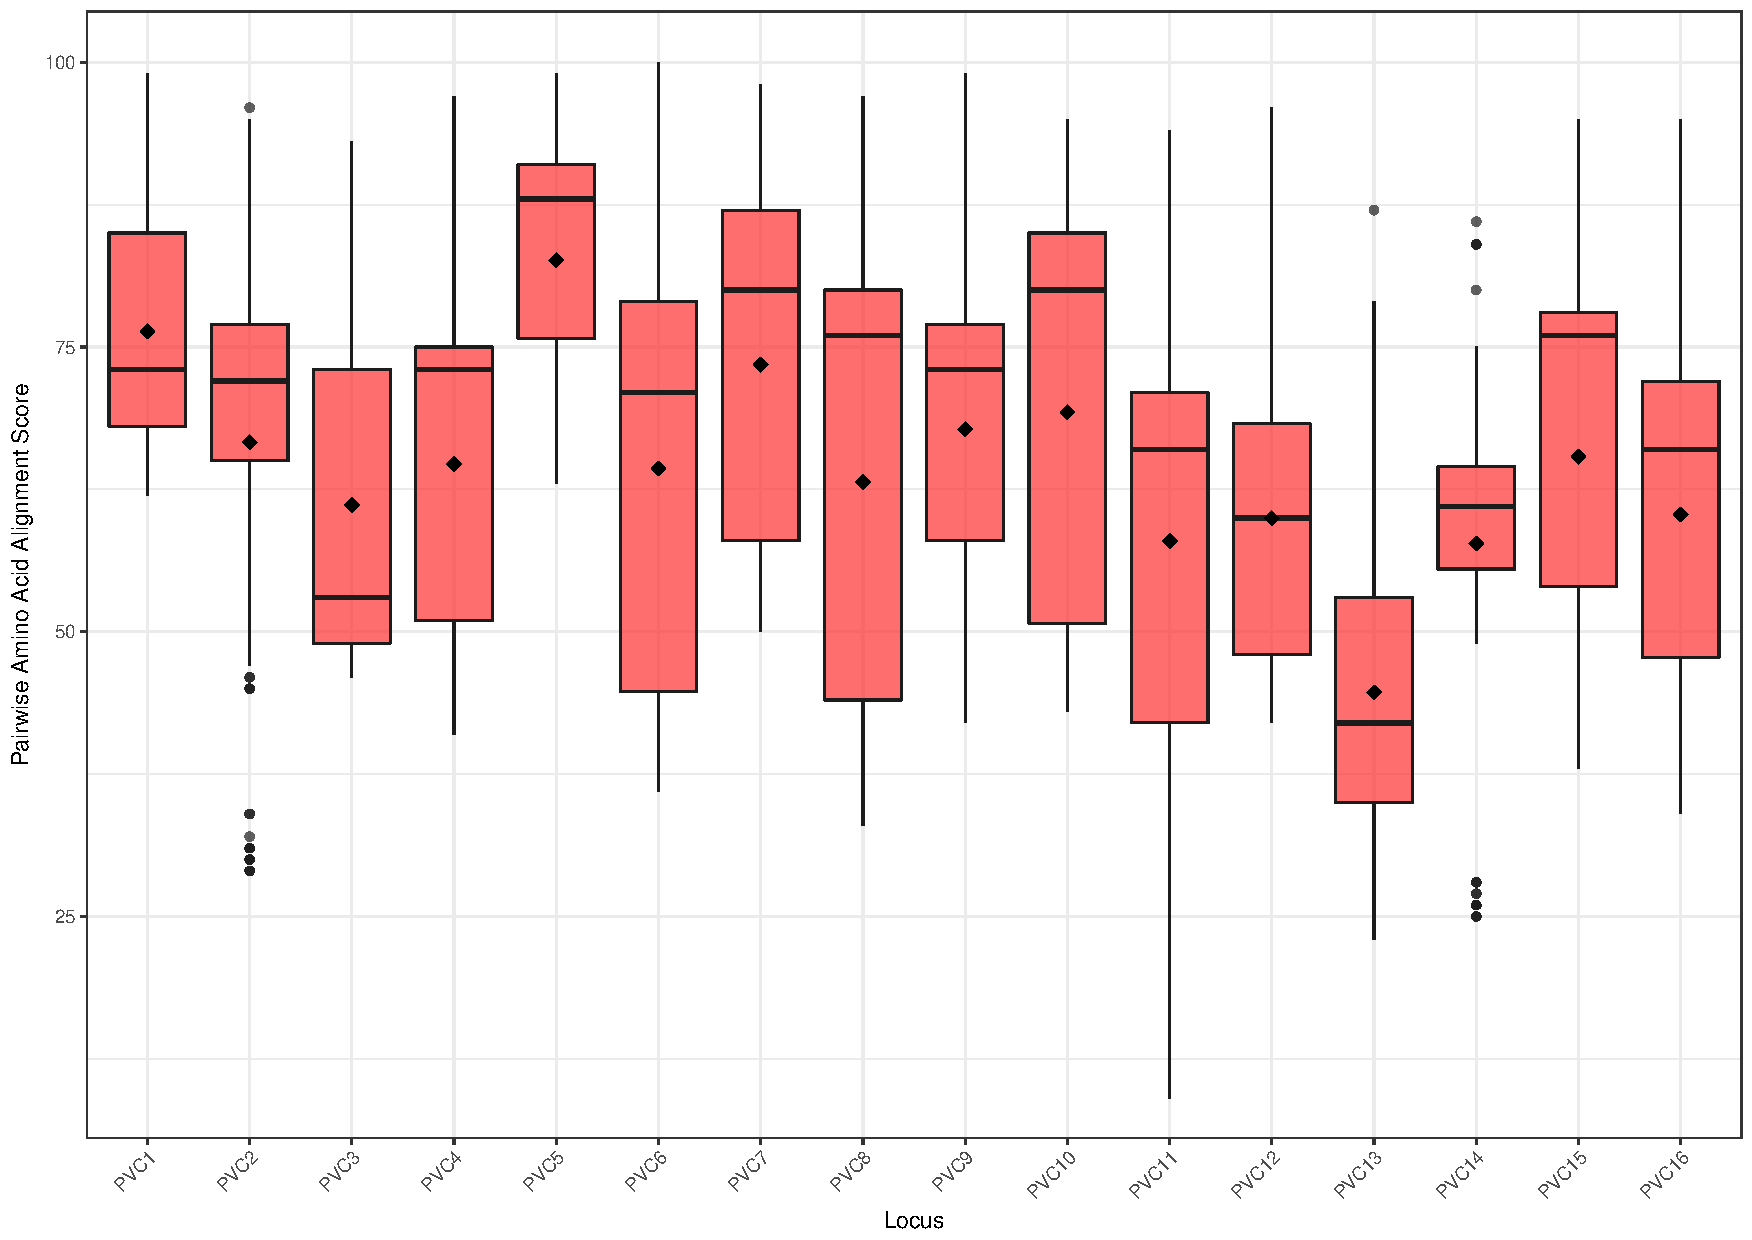
\includegraphics[width=0.8\textwidth, trim={0, 0, 0, 0}, clip]{/Users/joehealey/Documents/Warwick/PhD/Thesis/chapters/chapter4/img/Score_boxplot_with_means.pdf}
	\captionsetup{singlelinecheck=off, justification=justified, font=footnotesize, aboveskip=10pt}
	\caption[Pairwise Amino Acid Similarity Scores for PVC Proteins]{\textsc{\normalsize Pairwise amino acid similarity of all-vs-all genes for each PVC locus}\vspace{0.1cm} \newline Pairwise alignment similarity scores of a multiple sequence alignment of all the sequences within a given syntenic position. This demonstrates the distribution of similarity within a locus, and highlights that there are significantly different PVC `alleles' due to their position as outliers. $\blacklozenge$ denotes the mean, $\bullet$ denotes extreme outliers outside 1.5$\times$ the interquartile range for the sample, and the black line denotes the median.}
	\label{AAID}
\end{figure}


\newpage
\subsection{Gene Trees}

\begin{figure}[h!]
	\centering
	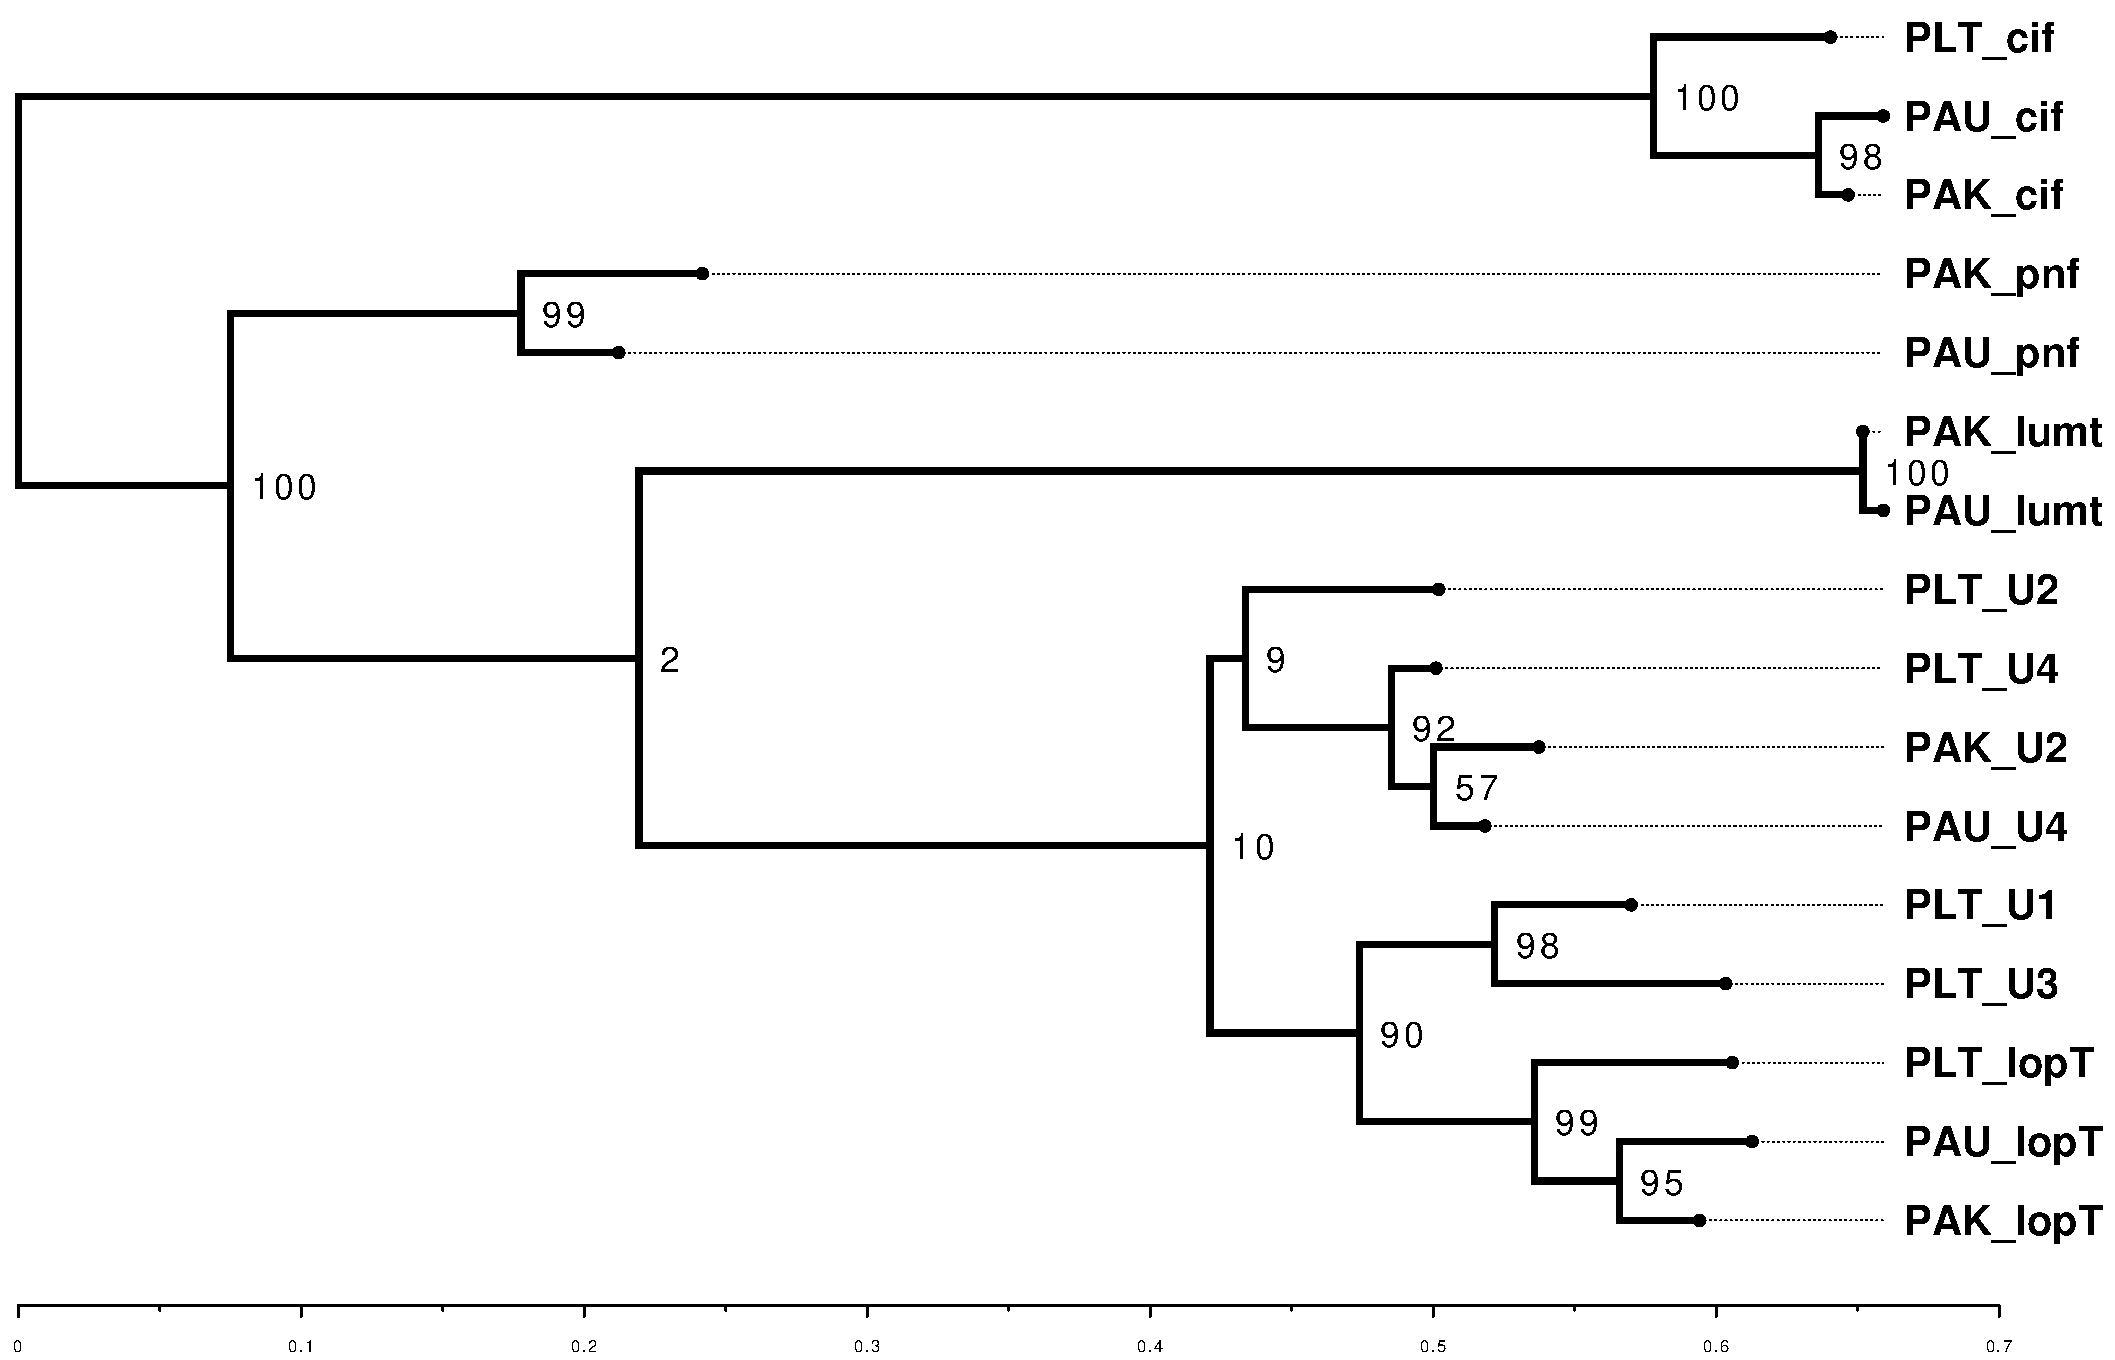
\includegraphics[width=0.95\textwidth]{/Users/joehealey/Documents/Warwick/PhD/Thesis/chapters/chapter4/img/PVC1.pdf}
	\captionsetup{singlelinecheck=off, justification=justified, font=footnotesize, aboveskip=19pt}
	\caption[Gene tree for the first PVC locus]{\textsc{\normalsize Maximum-likelihood tree of the locus position (PVC1) from each operon.}}
	\label{pvc1tree}
\end{figure}
\hfill
\begin{figure}[h!]
	\centering
	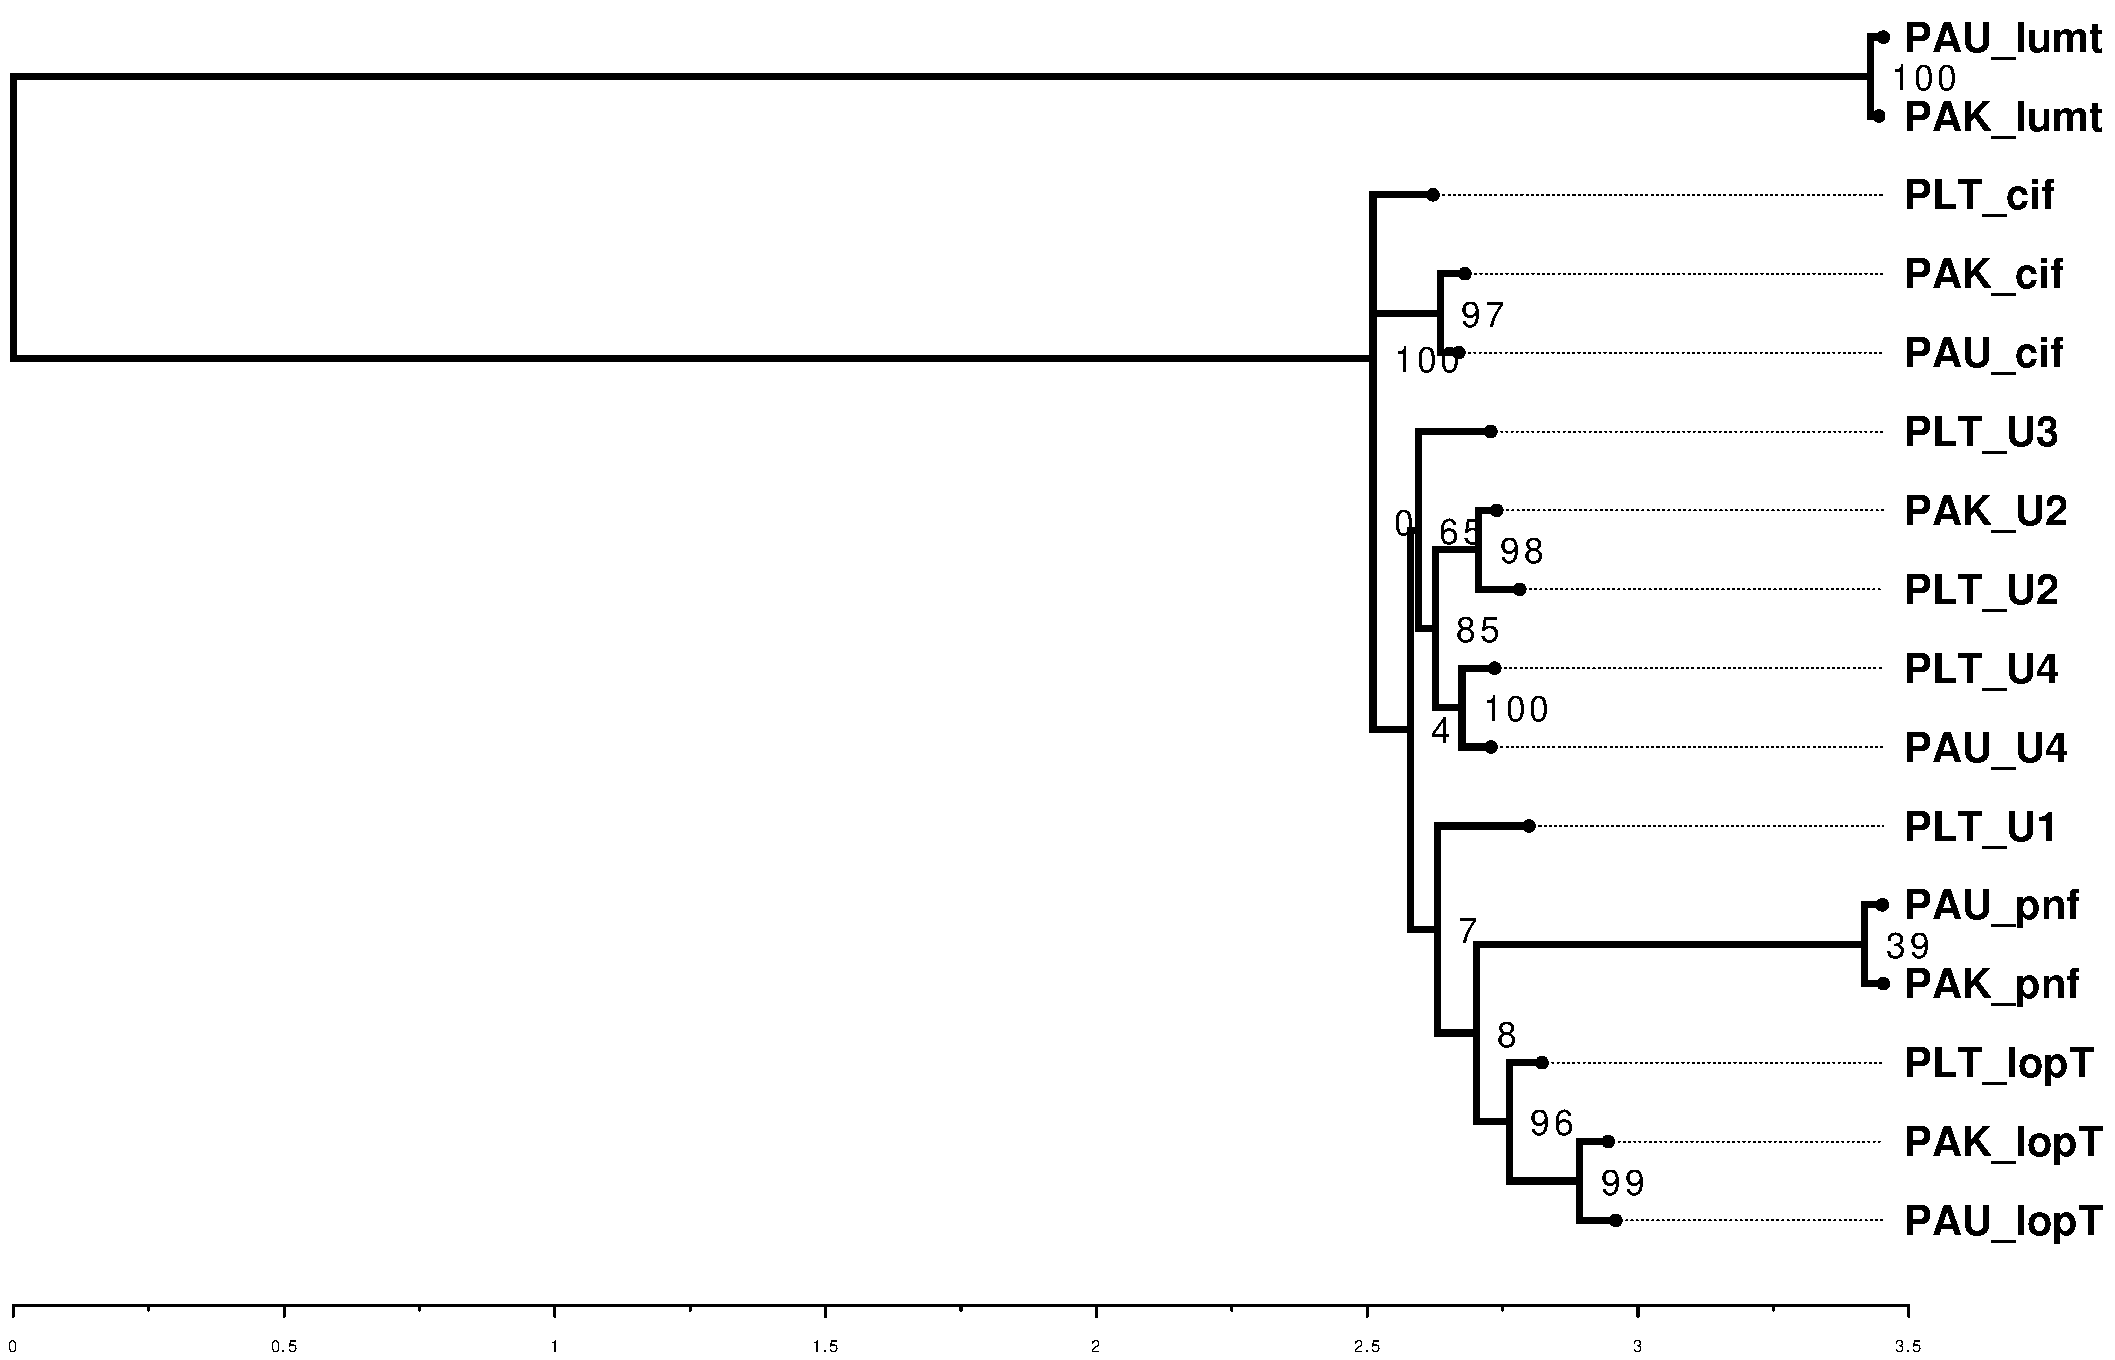
\includegraphics[width=0.95\textwidth]{/Users/joehealey/Documents/Warwick/PhD/Thesis/chapters/chapter4/img/PVC2.pdf}
	\captionsetup{singlelinecheck=off, justification=justified, font=footnotesize, aboveskip=19pt}
	\caption[Gene tree for the second PVC locus]{\textsc{\normalsize Maximum-likelihood tree of the locus position (PVC2) from each operon.}}
	\label{pvc2tree}
\end{figure}

\newpage

\begin{figure}[h!]
	\centering
	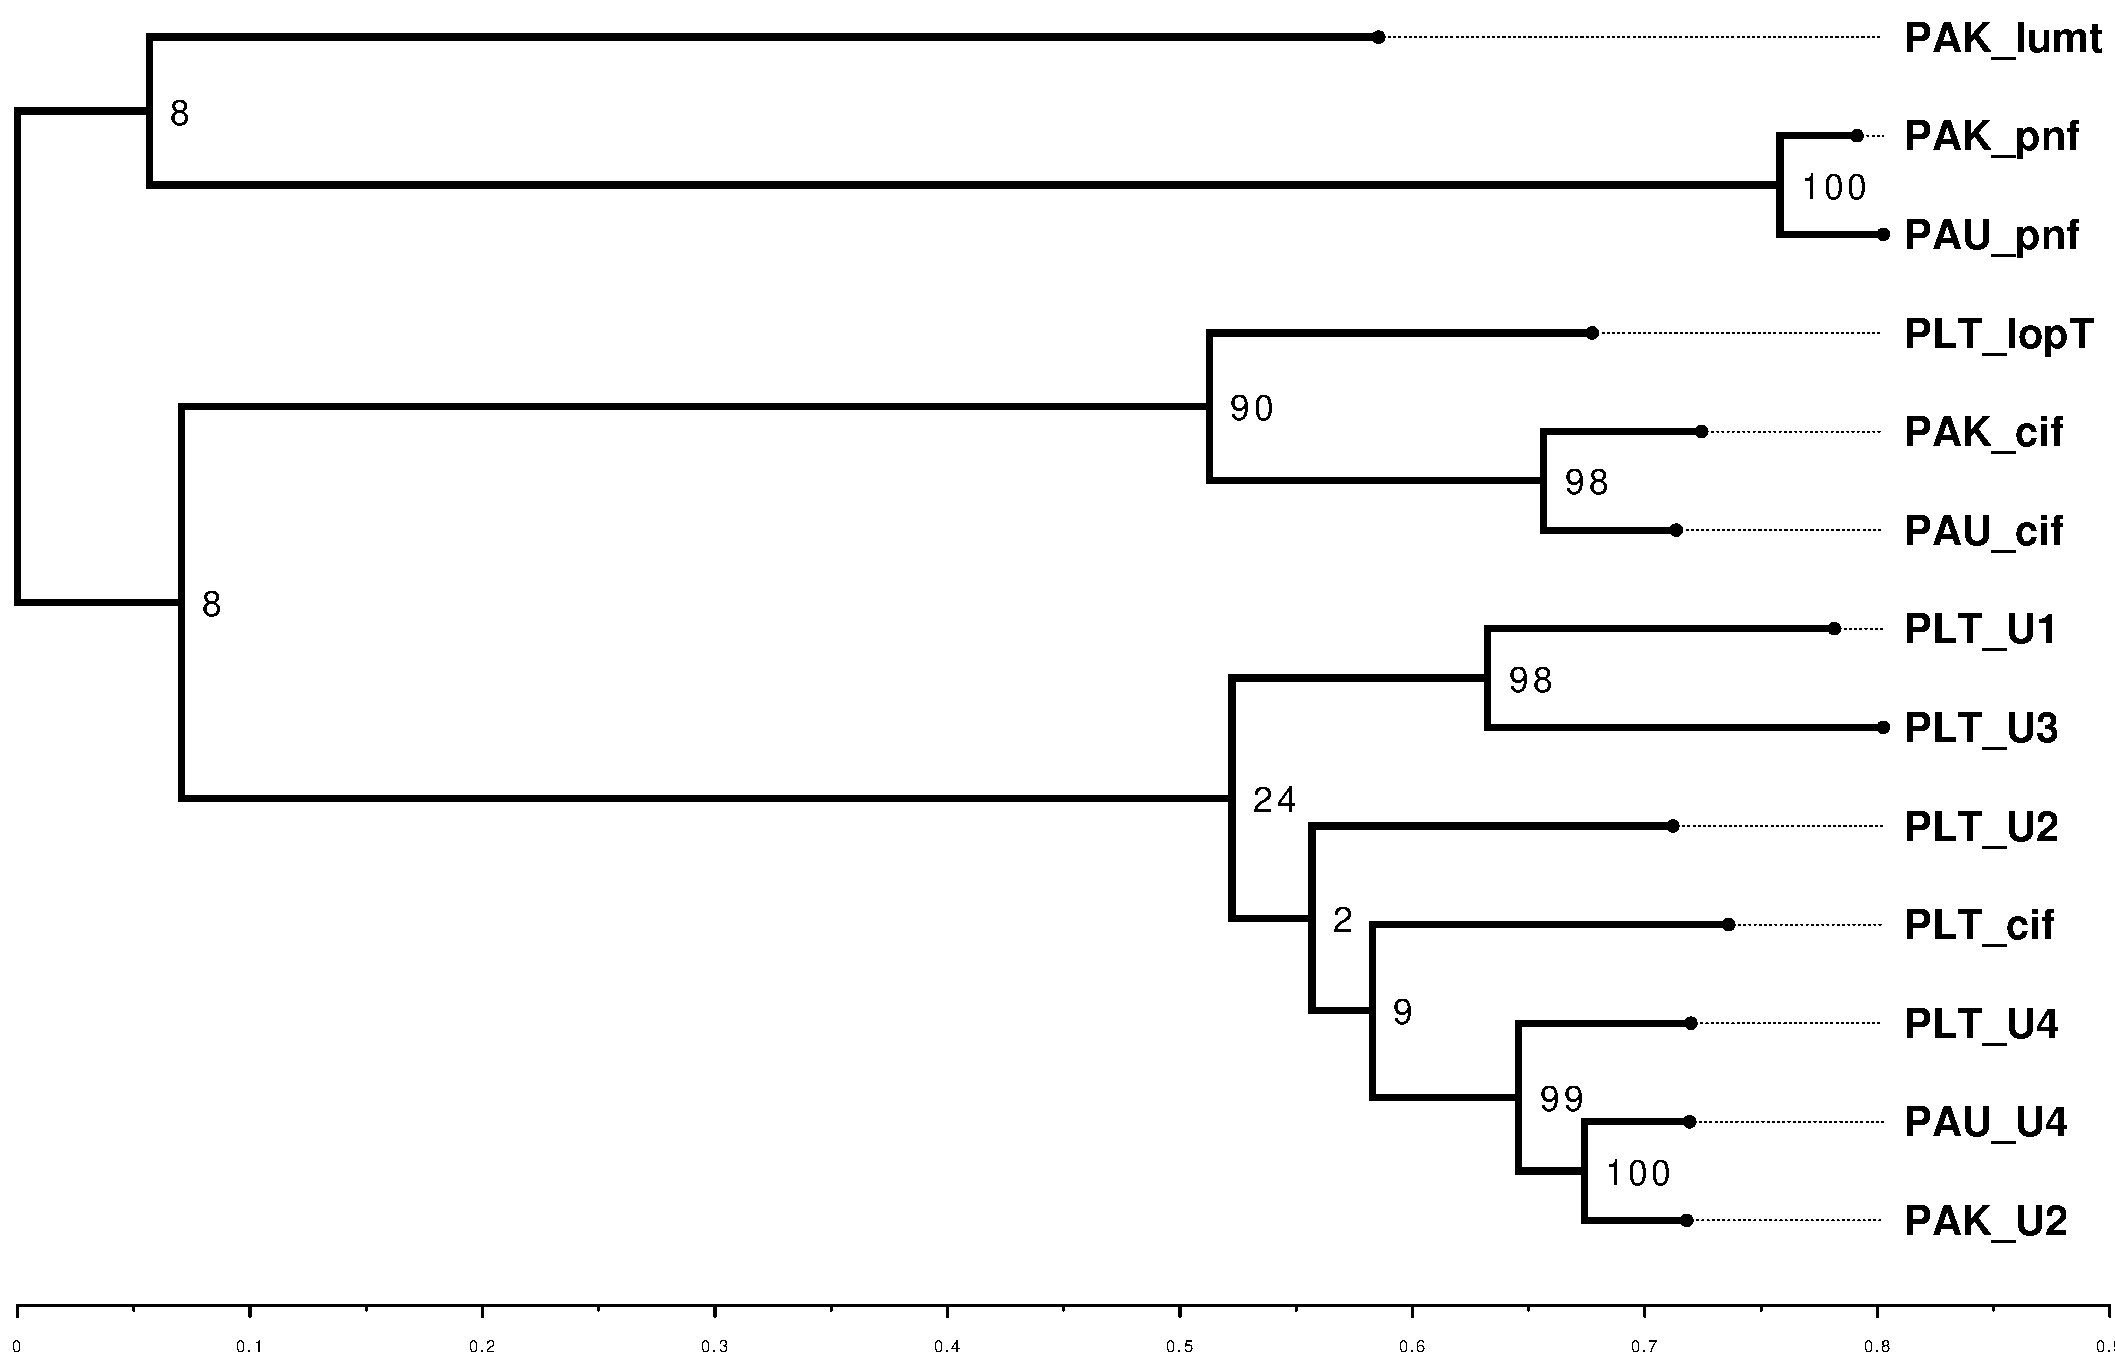
\includegraphics[width=0.95\textwidth]{/Users/joehealey/Documents/Warwick/PhD/Thesis/chapters/chapter4/img/PVC3.pdf}
	\captionsetup{singlelinecheck=off, justification=justified, font=footnotesize, aboveskip=19pt}
	\caption[Gene tree for the third PVC locus]{\textsc{\normalsize Maximum-likelihood tree of the locus position (PVC3) from each operon.}}
	\label{pvc3tree}
\end{figure}
\hfill
\begin{figure}[h!]
	\centering
	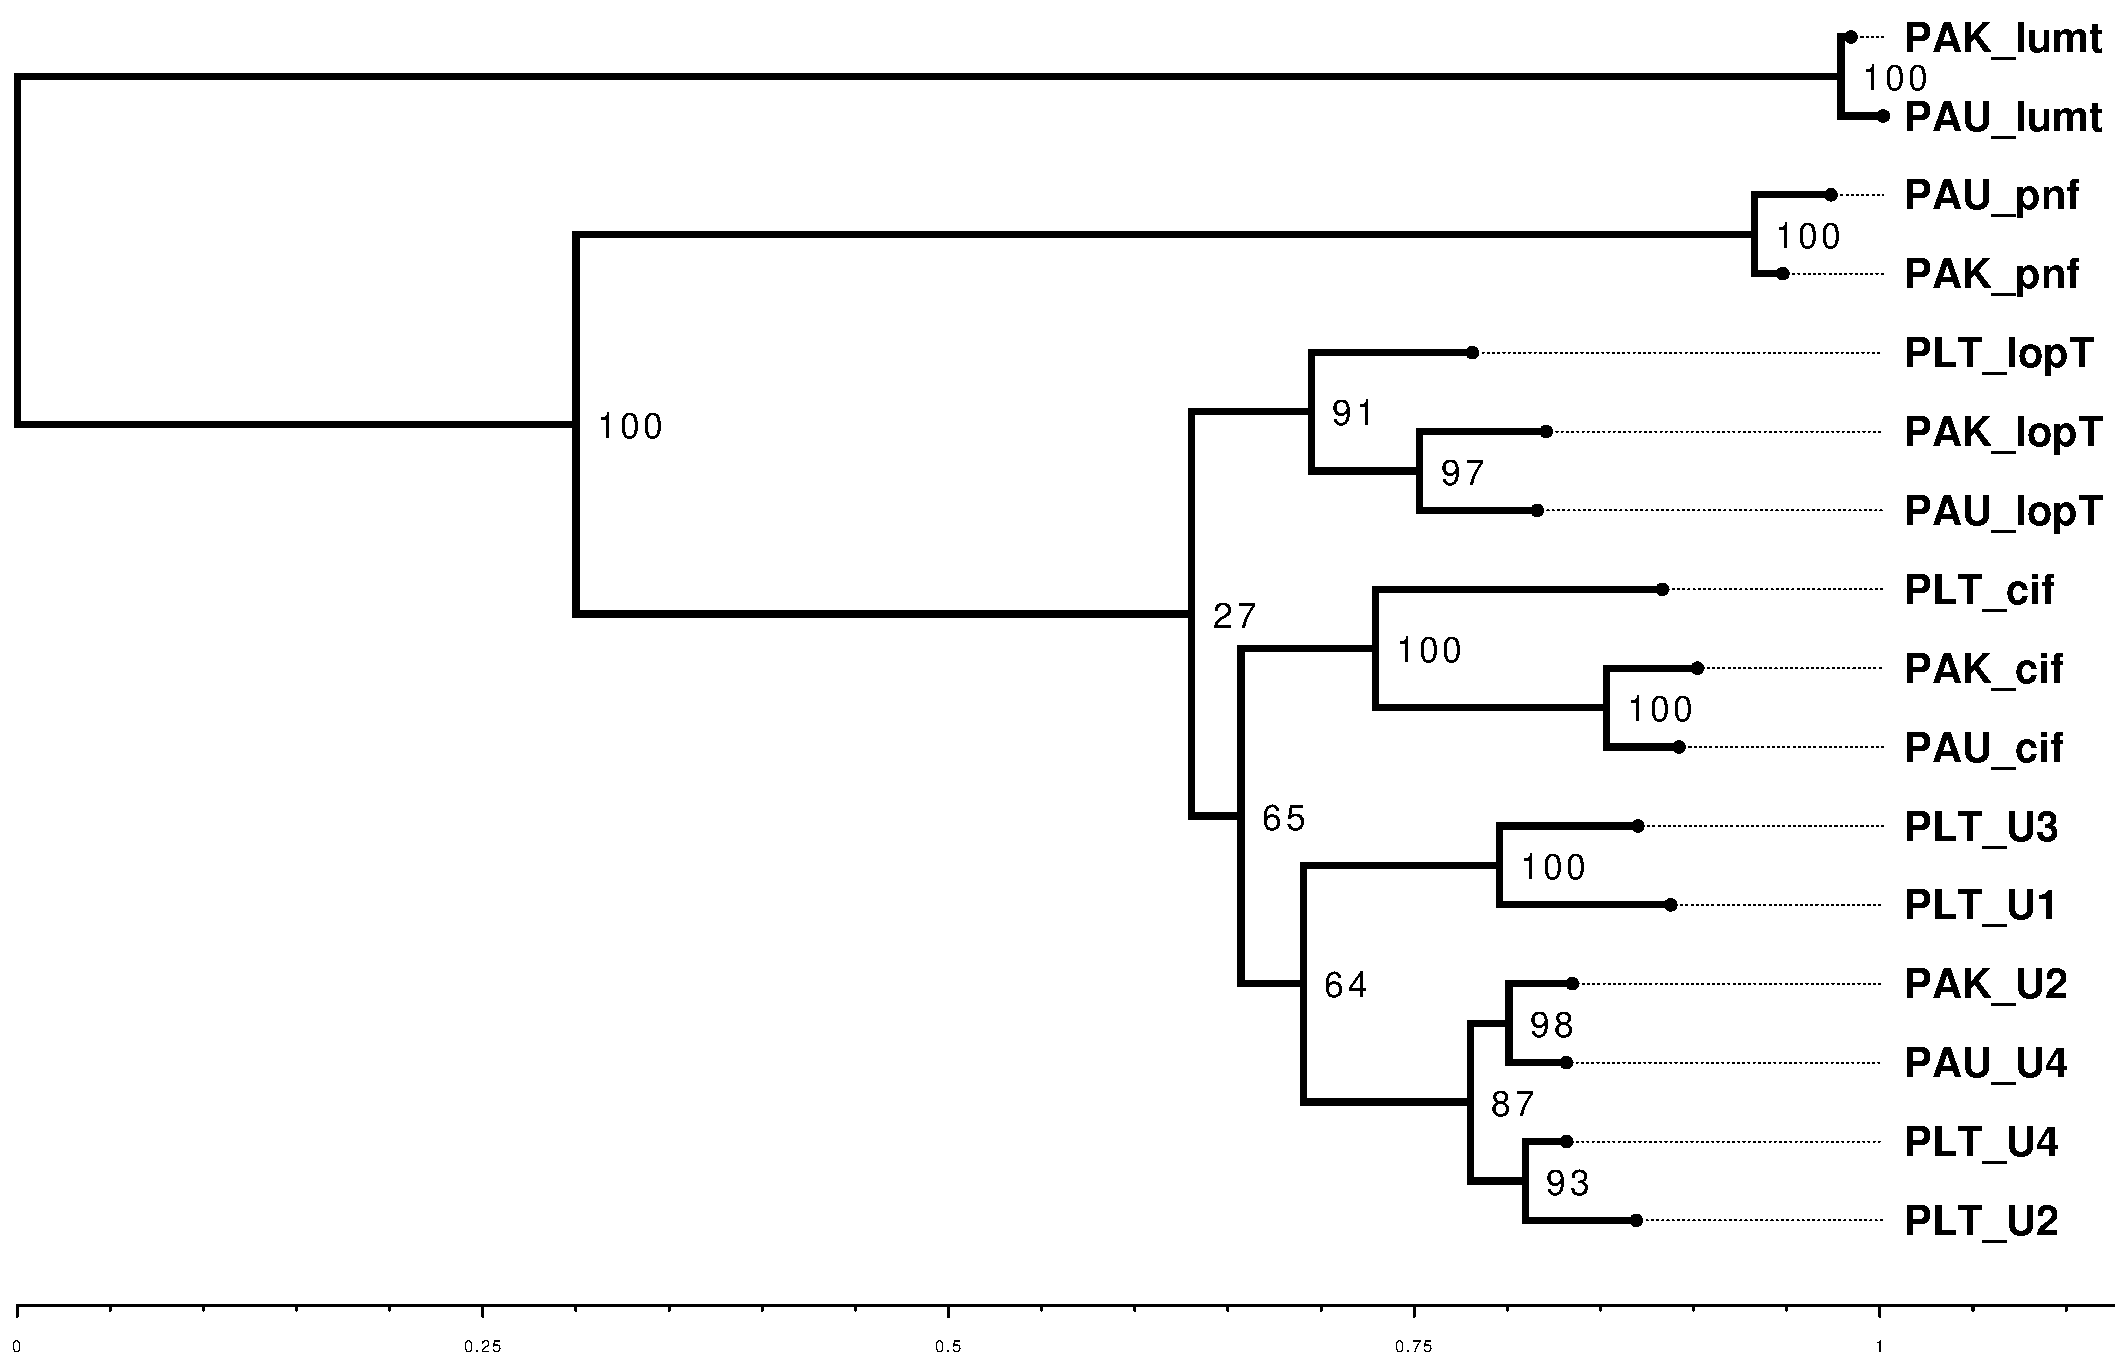
\includegraphics[width=0.95\textwidth]{/Users/joehealey/Documents/Warwick/PhD/Thesis/chapters/chapter4/img/PVC4.pdf}
	\captionsetup{singlelinecheck=off, justification=justified, font=footnotesize, aboveskip=19pt}
	\caption[Gene tree for the fourth PVC locus]{\textsc{\normalsize Maximum-likelihood tree of the locus position (PVC4) from each operon.}}
	\label{pvc4tree}
\end{figure}

\newpage

\begin{figure}[h!]
	\centering
	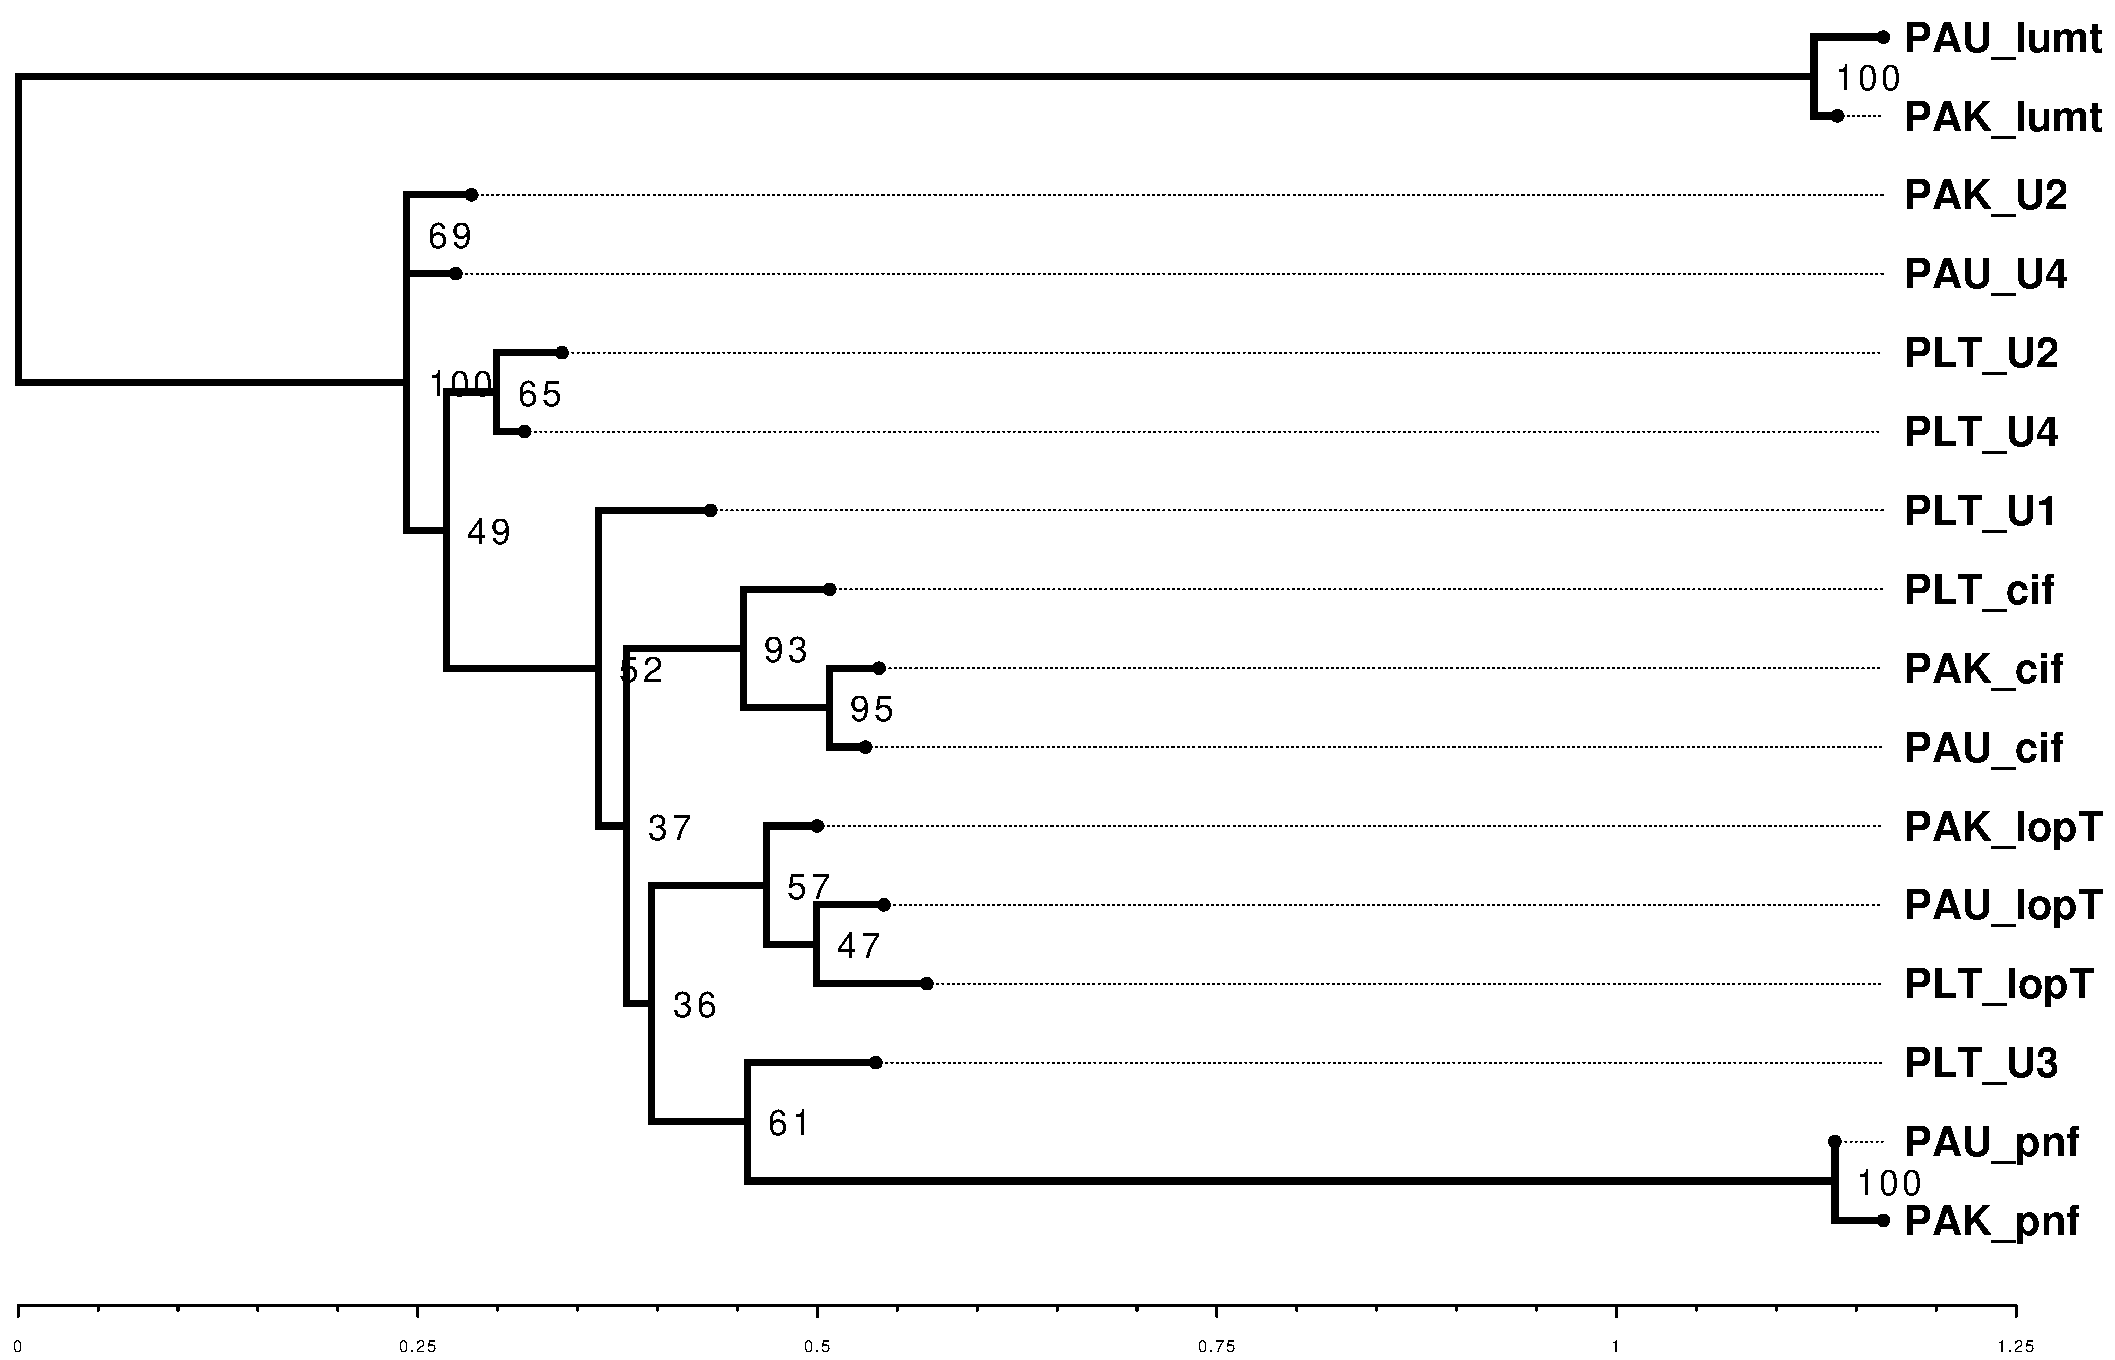
\includegraphics[width=0.95\textwidth]{/Users/joehealey/Documents/Warwick/PhD/Thesis/chapters/chapter4/img/PVC5.pdf}
	\captionsetup{singlelinecheck=off, justification=justified, font=footnotesize, aboveskip=19pt}
	\caption[Gene tree for the fifth PVC locus]{\textsc{\normalsize Maximum-likelihood tree of the locus position (PVC5) from each operon.}}
	\label{pvc5tree}
\end{figure}
\hfill
\begin{figure}[h!]
	\centering
	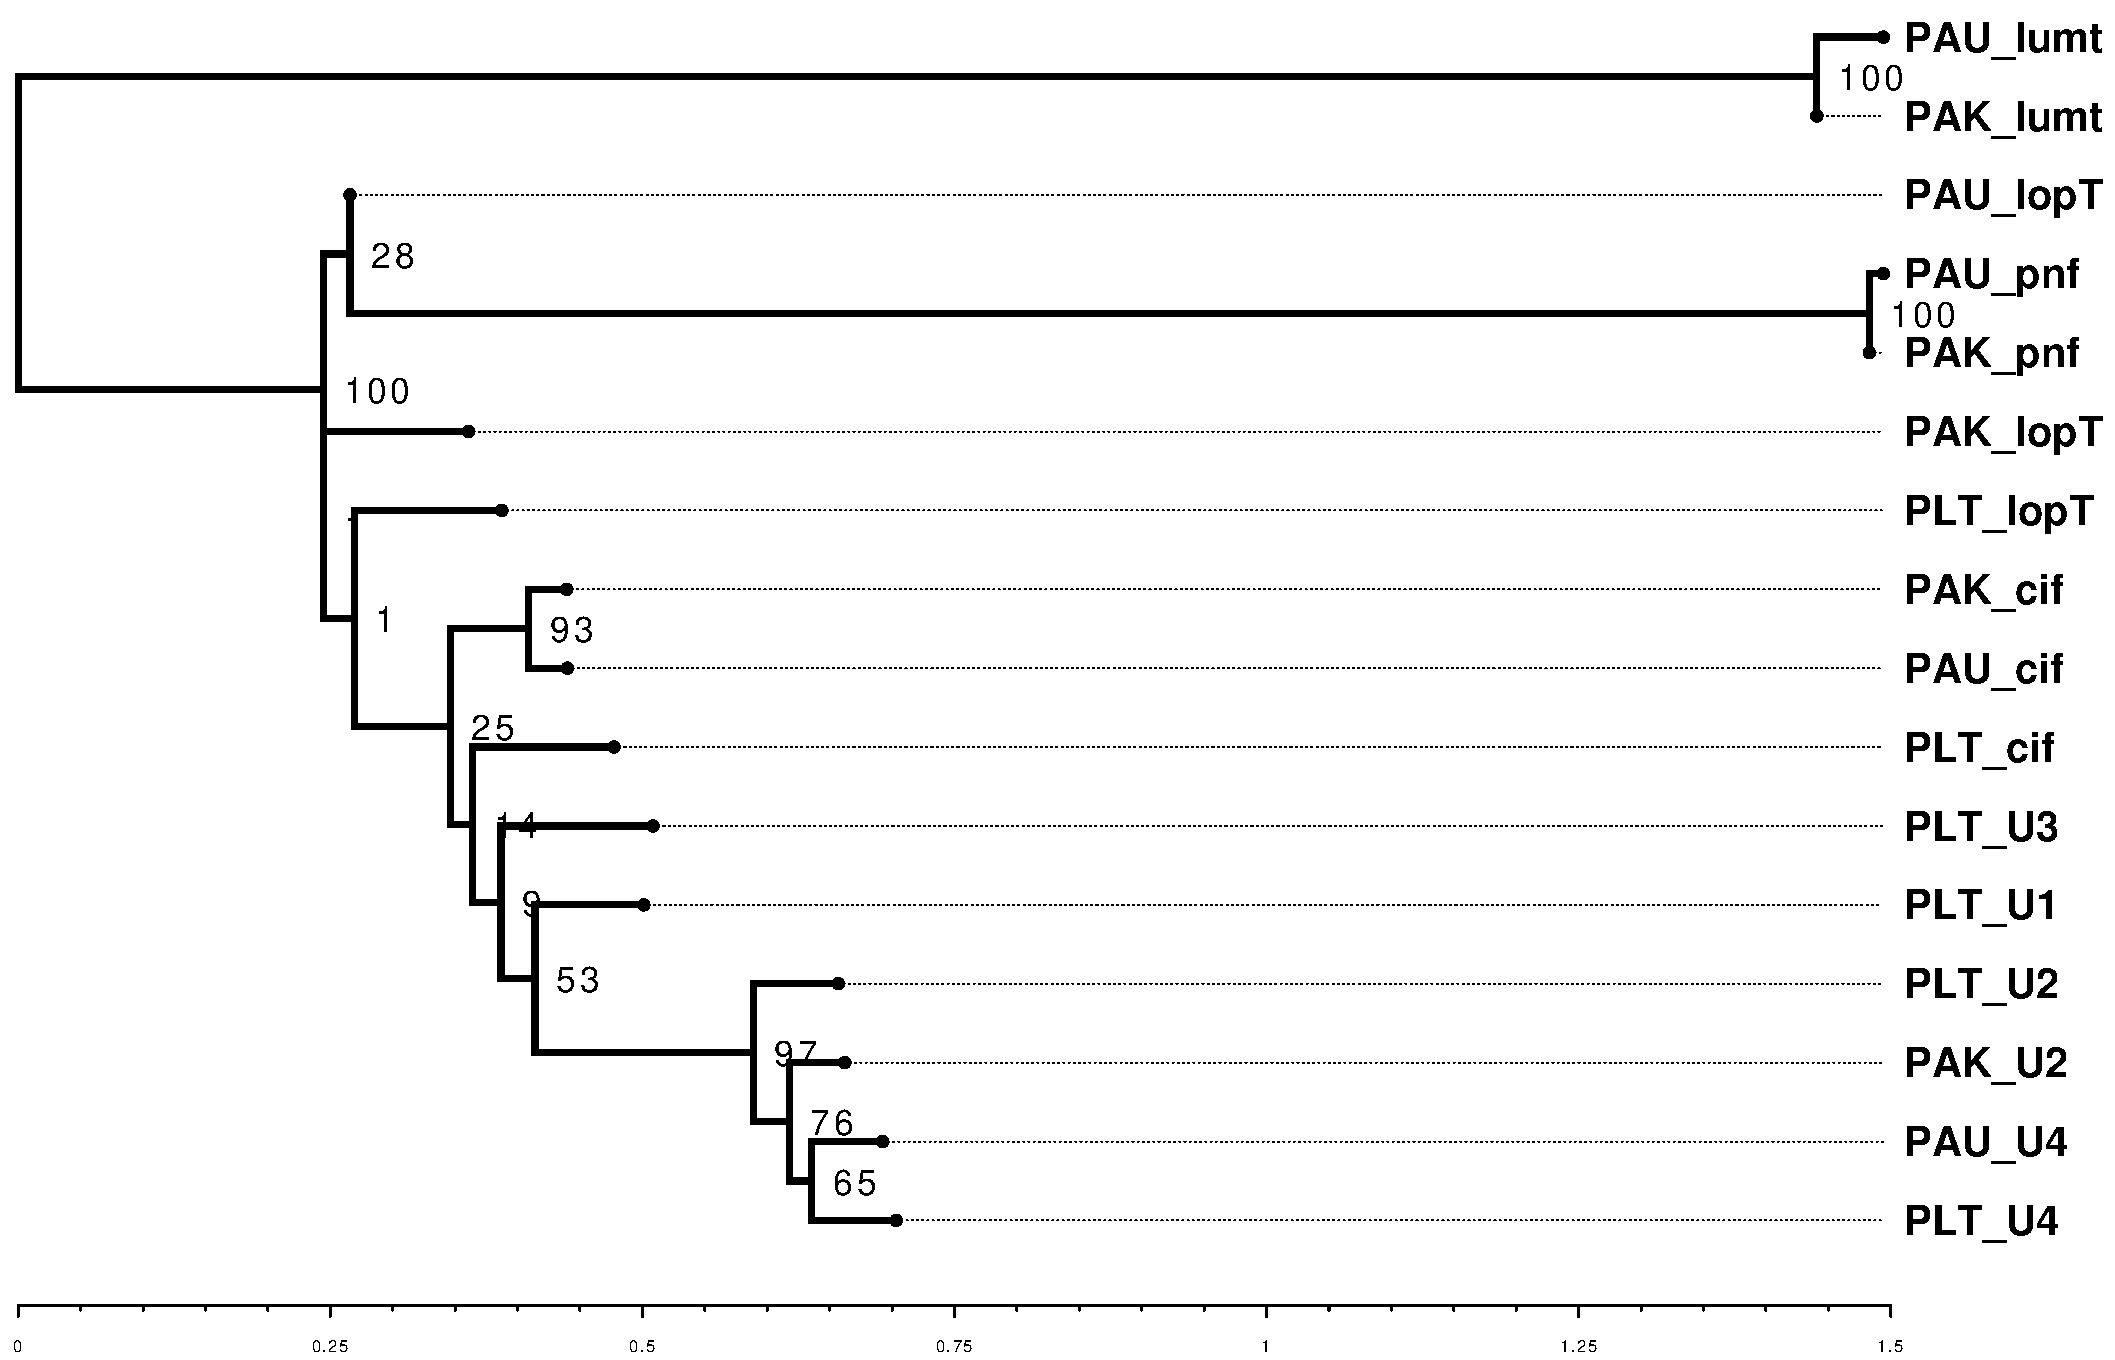
\includegraphics[width=0.95\textwidth]{/Users/joehealey/Documents/Warwick/PhD/Thesis/chapters/chapter4/img/PVC6.pdf}
	\captionsetup{singlelinecheck=off, justification=justified, font=footnotesize, aboveskip=19pt}
	\caption[Gene tree for the sixth PVC locus]{\textsc{\normalsize Maximum-likelihood tree of the locus position (PVC6) from each operon.}}
	\label{pvc6tree}
\end{figure}

\newpage

\begin{figure}[h!]
	\centering
	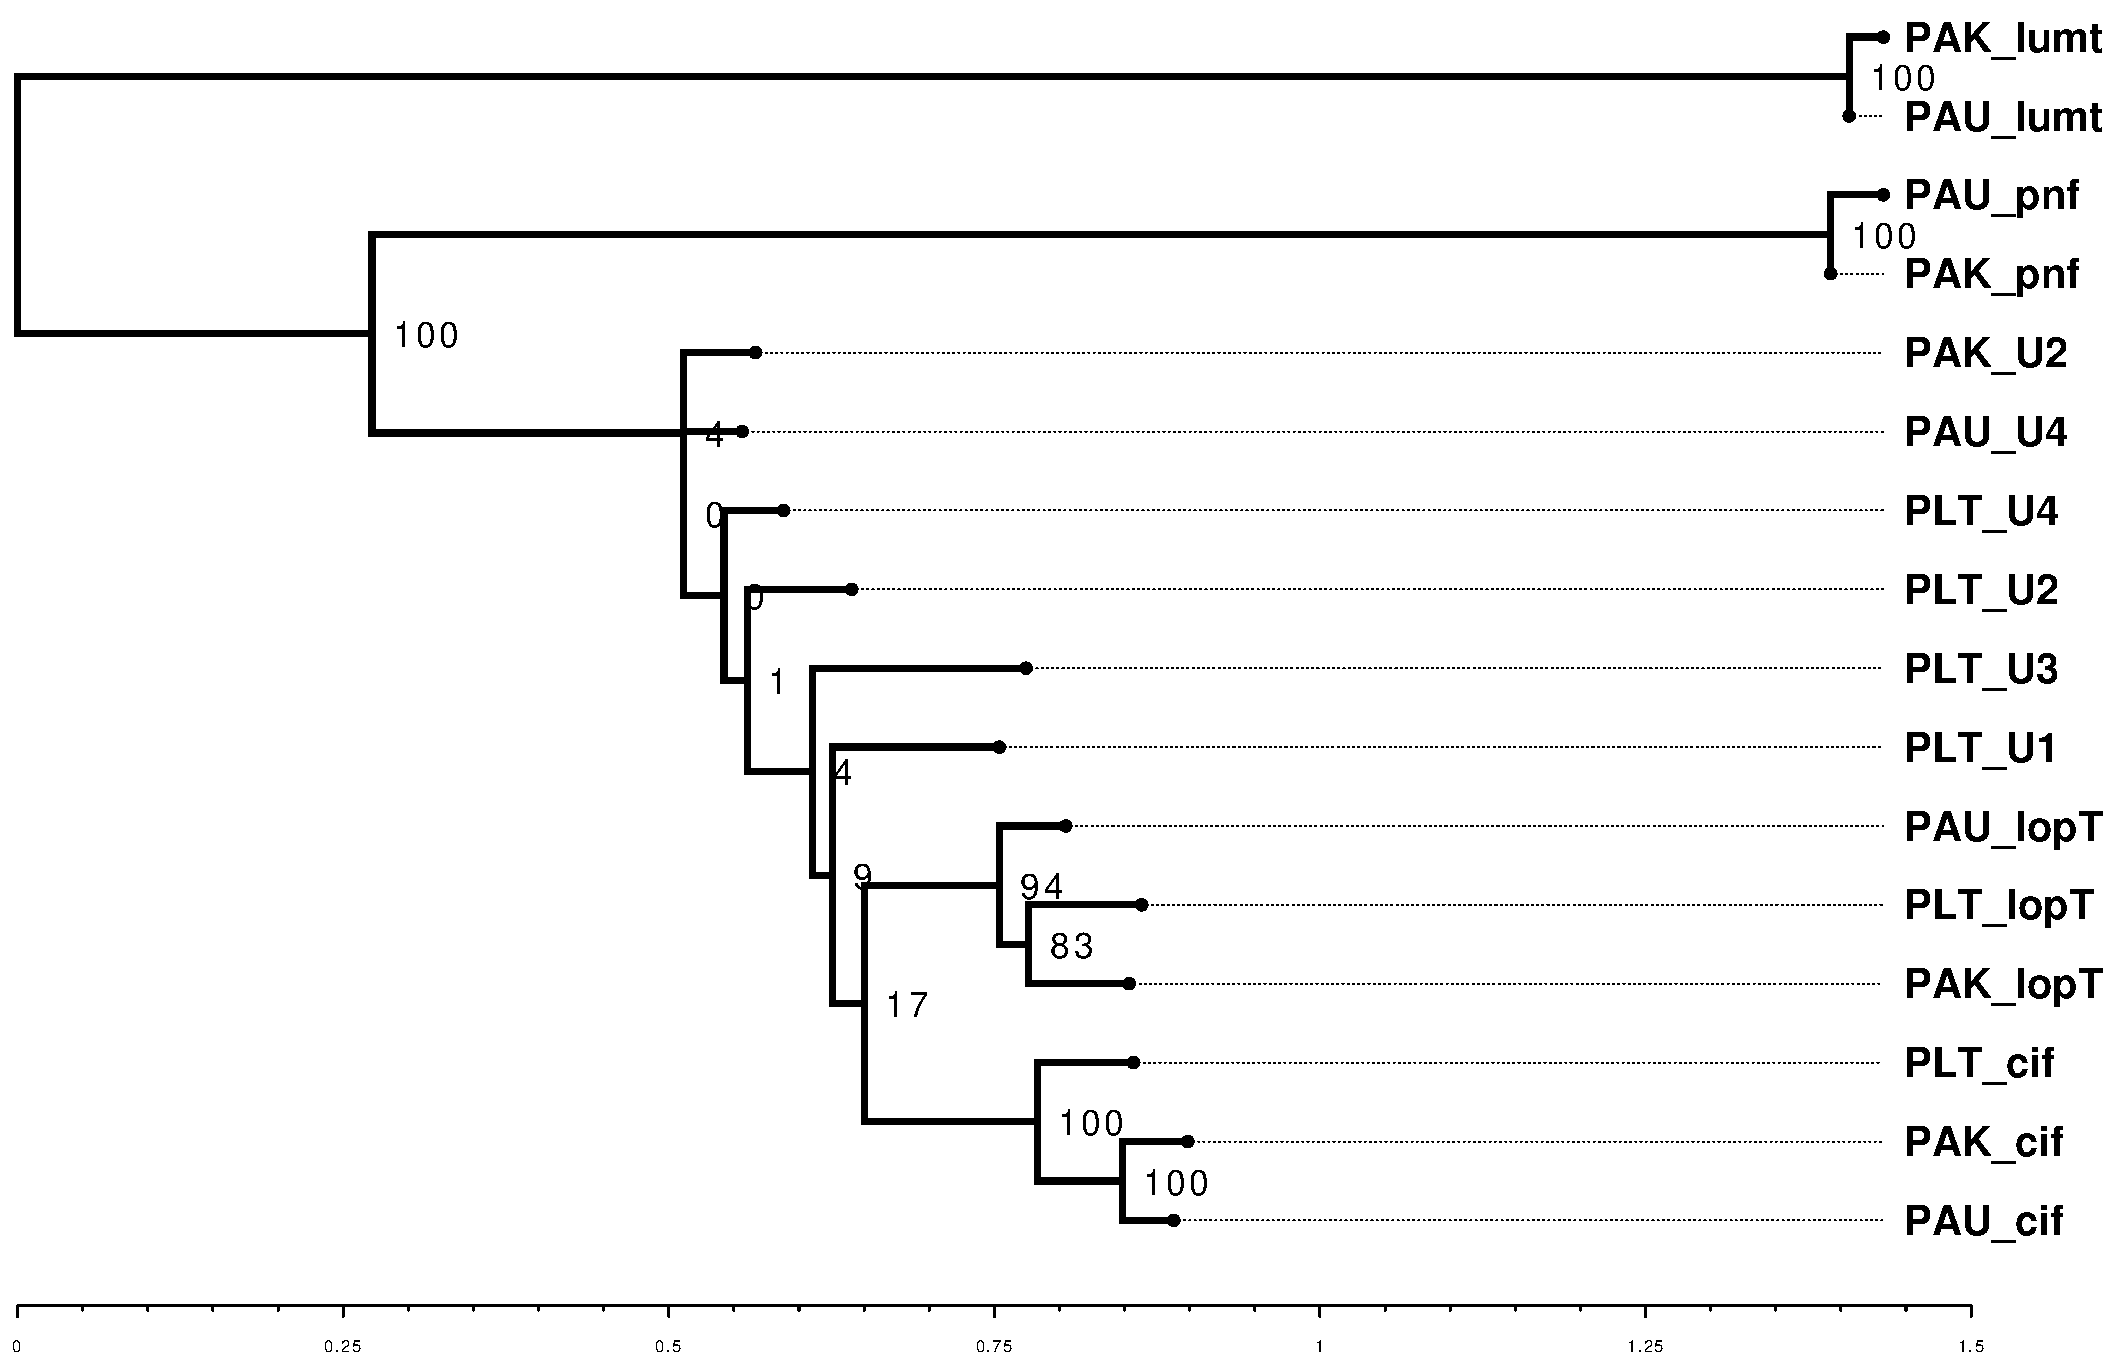
\includegraphics[width=0.95\textwidth]{/Users/joehealey/Documents/Warwick/PhD/Thesis/chapters/chapter4/img/PVC7.pdf}
	\captionsetup{singlelinecheck=off, justification=justified, font=footnotesize, aboveskip=19pt}
	\caption[Gene tree for the seventh PVC locus]{\textsc{\normalsize Maximum-likelihood tree of the locus position (PVC7) from each operon.}}
	\label{pvc7tree}
\end{figure}
\hfill
\begin{figure}[h!]
	\centering
	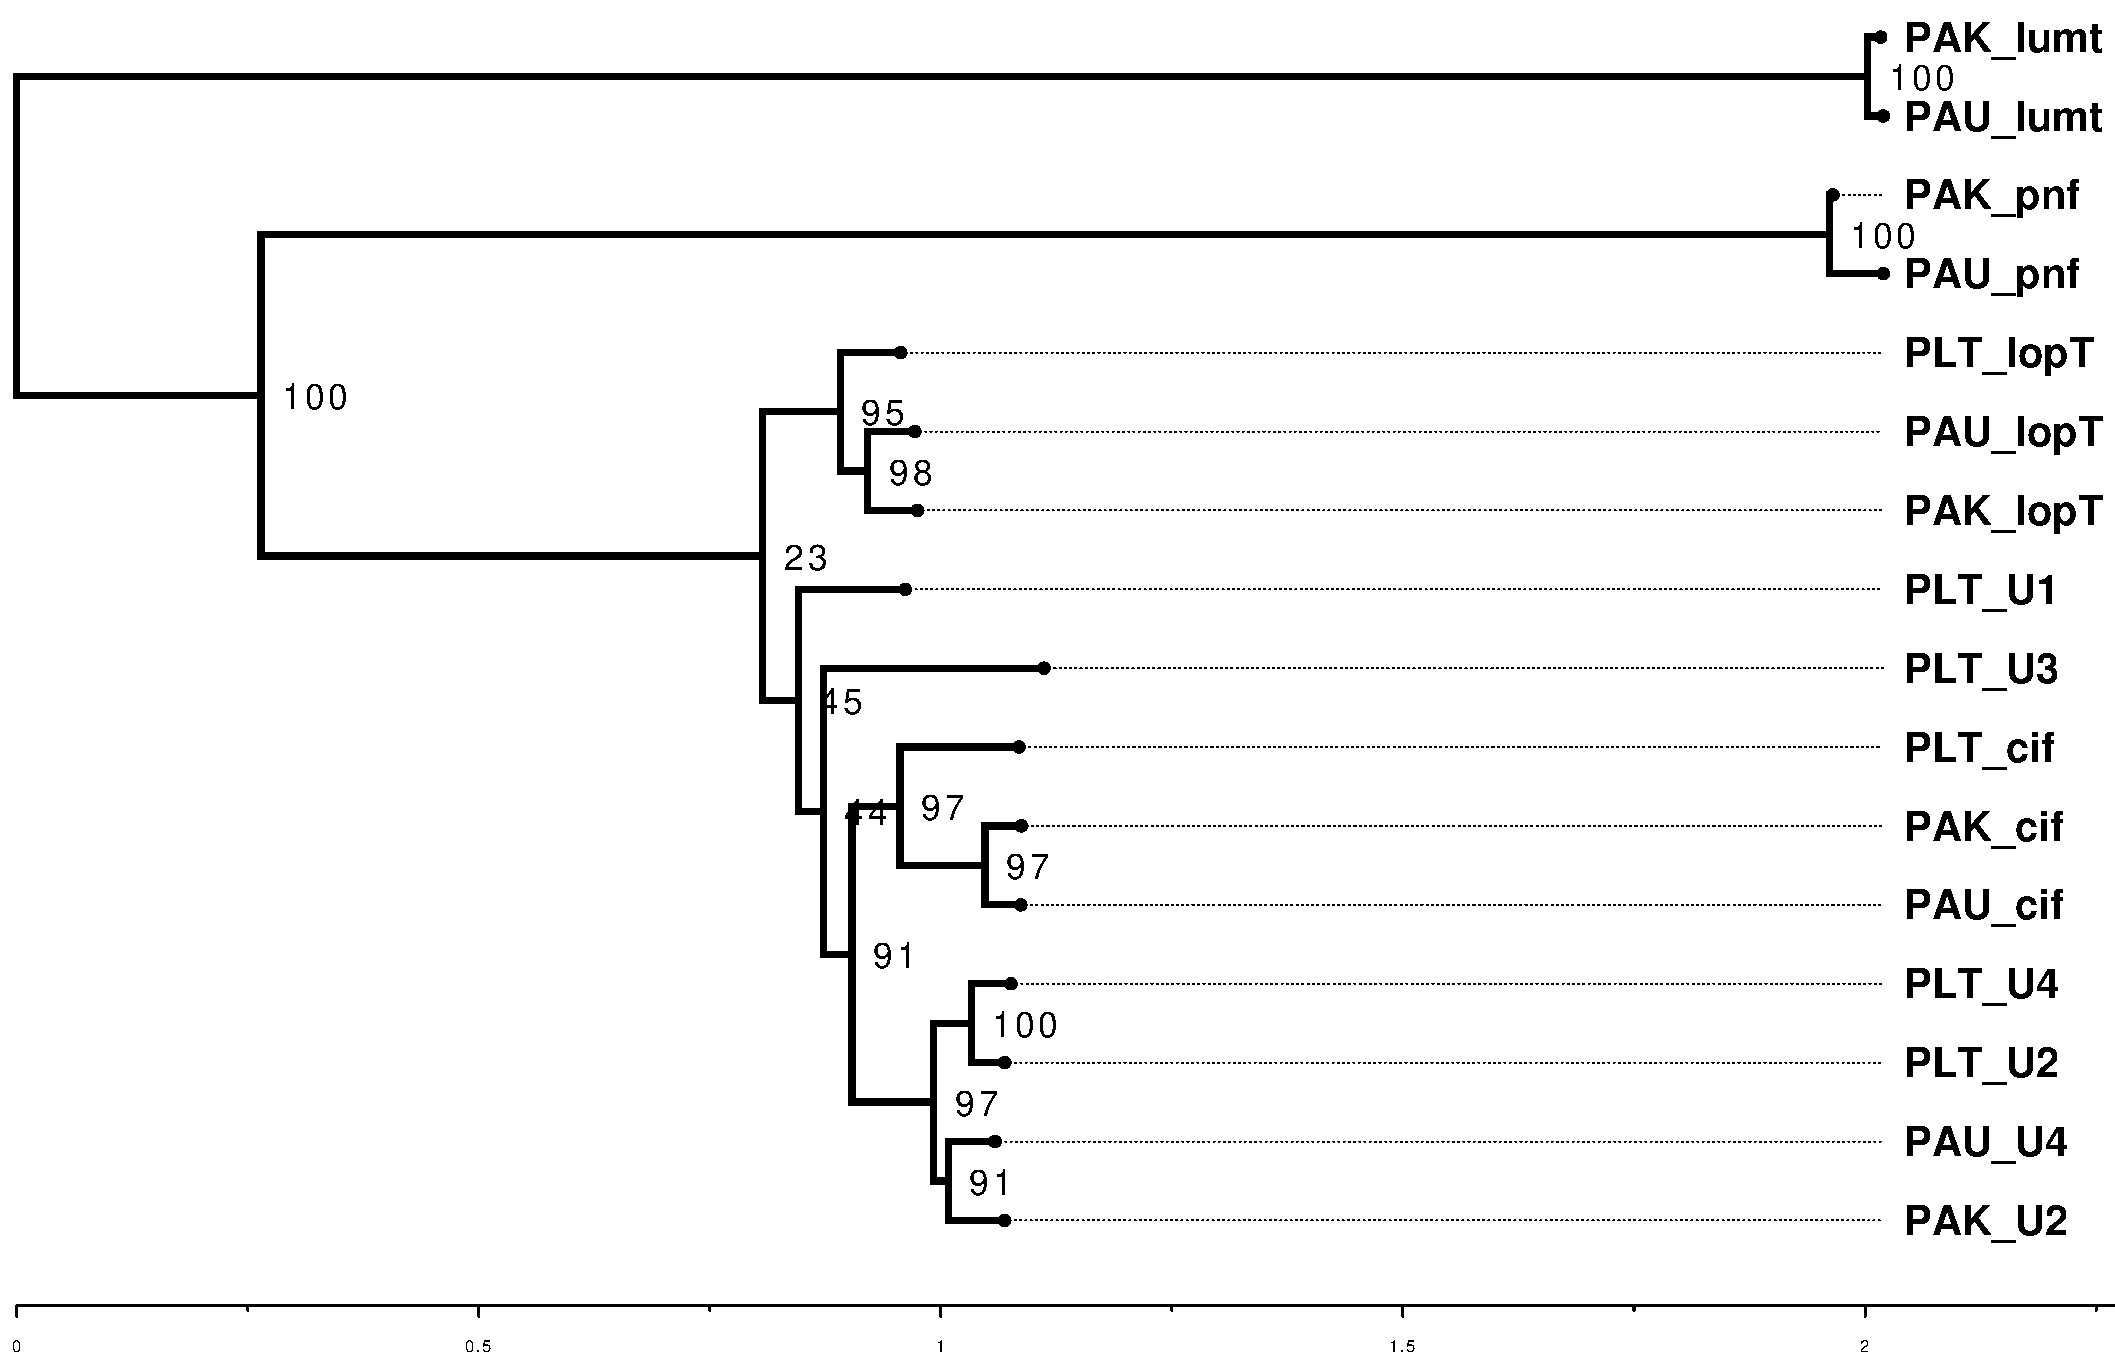
\includegraphics[width=0.95\textwidth]{/Users/joehealey/Documents/Warwick/PhD/Thesis/chapters/chapter4/img/PVC8.pdf}
	\captionsetup{singlelinecheck=off, justification=justified, font=footnotesize, aboveskip=19pt}
	\caption[Gene tree for the eighth PVC locus]{\textsc{\normalsize Maximum-likelihood tree of the locus position (PVC8) from each operon.}}
	\label{pvc8tree}
\end{figure}

\newpage
\begin{figure}[h!]
	\centering
	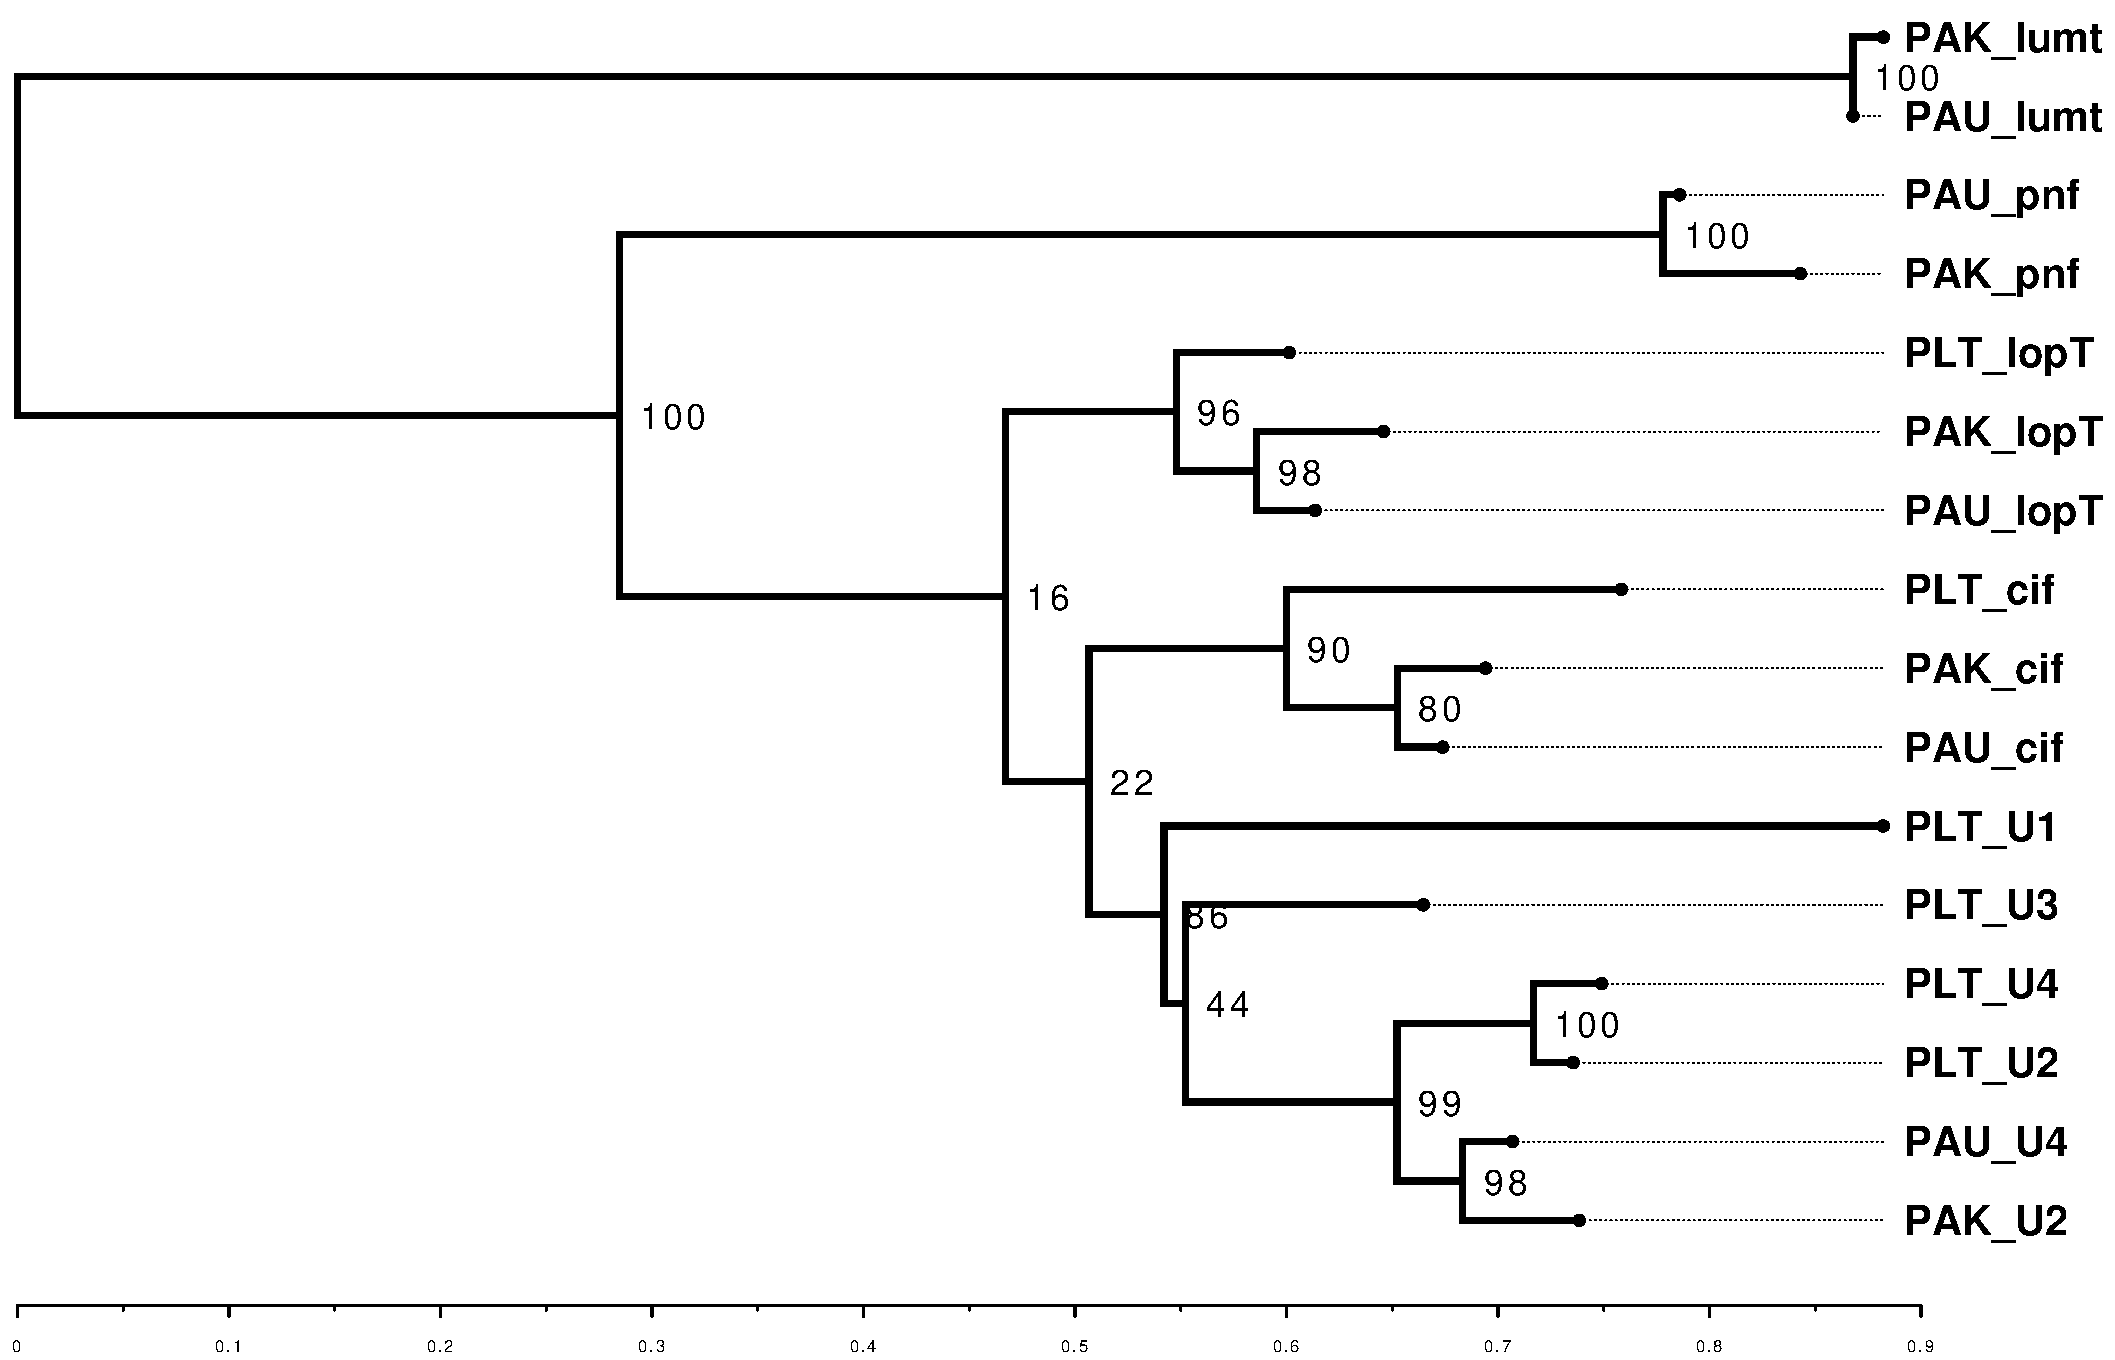
\includegraphics[width=0.95\textwidth]{/Users/joehealey/Documents/Warwick/PhD/Thesis/chapters/chapter4/img/PVC9.pdf}
	\captionsetup{singlelinecheck=off, justification=justified, font=footnotesize, aboveskip=19pt}
	\caption[Gene tree for the ninth PVC locus]{\textsc{\normalsize Maximum-likelihood tree of the locus position (PVC9) from each operon.}}
	\label{pvc9tree}
\end{figure}
\hfill
\begin{figure}[h!]
	\centering
	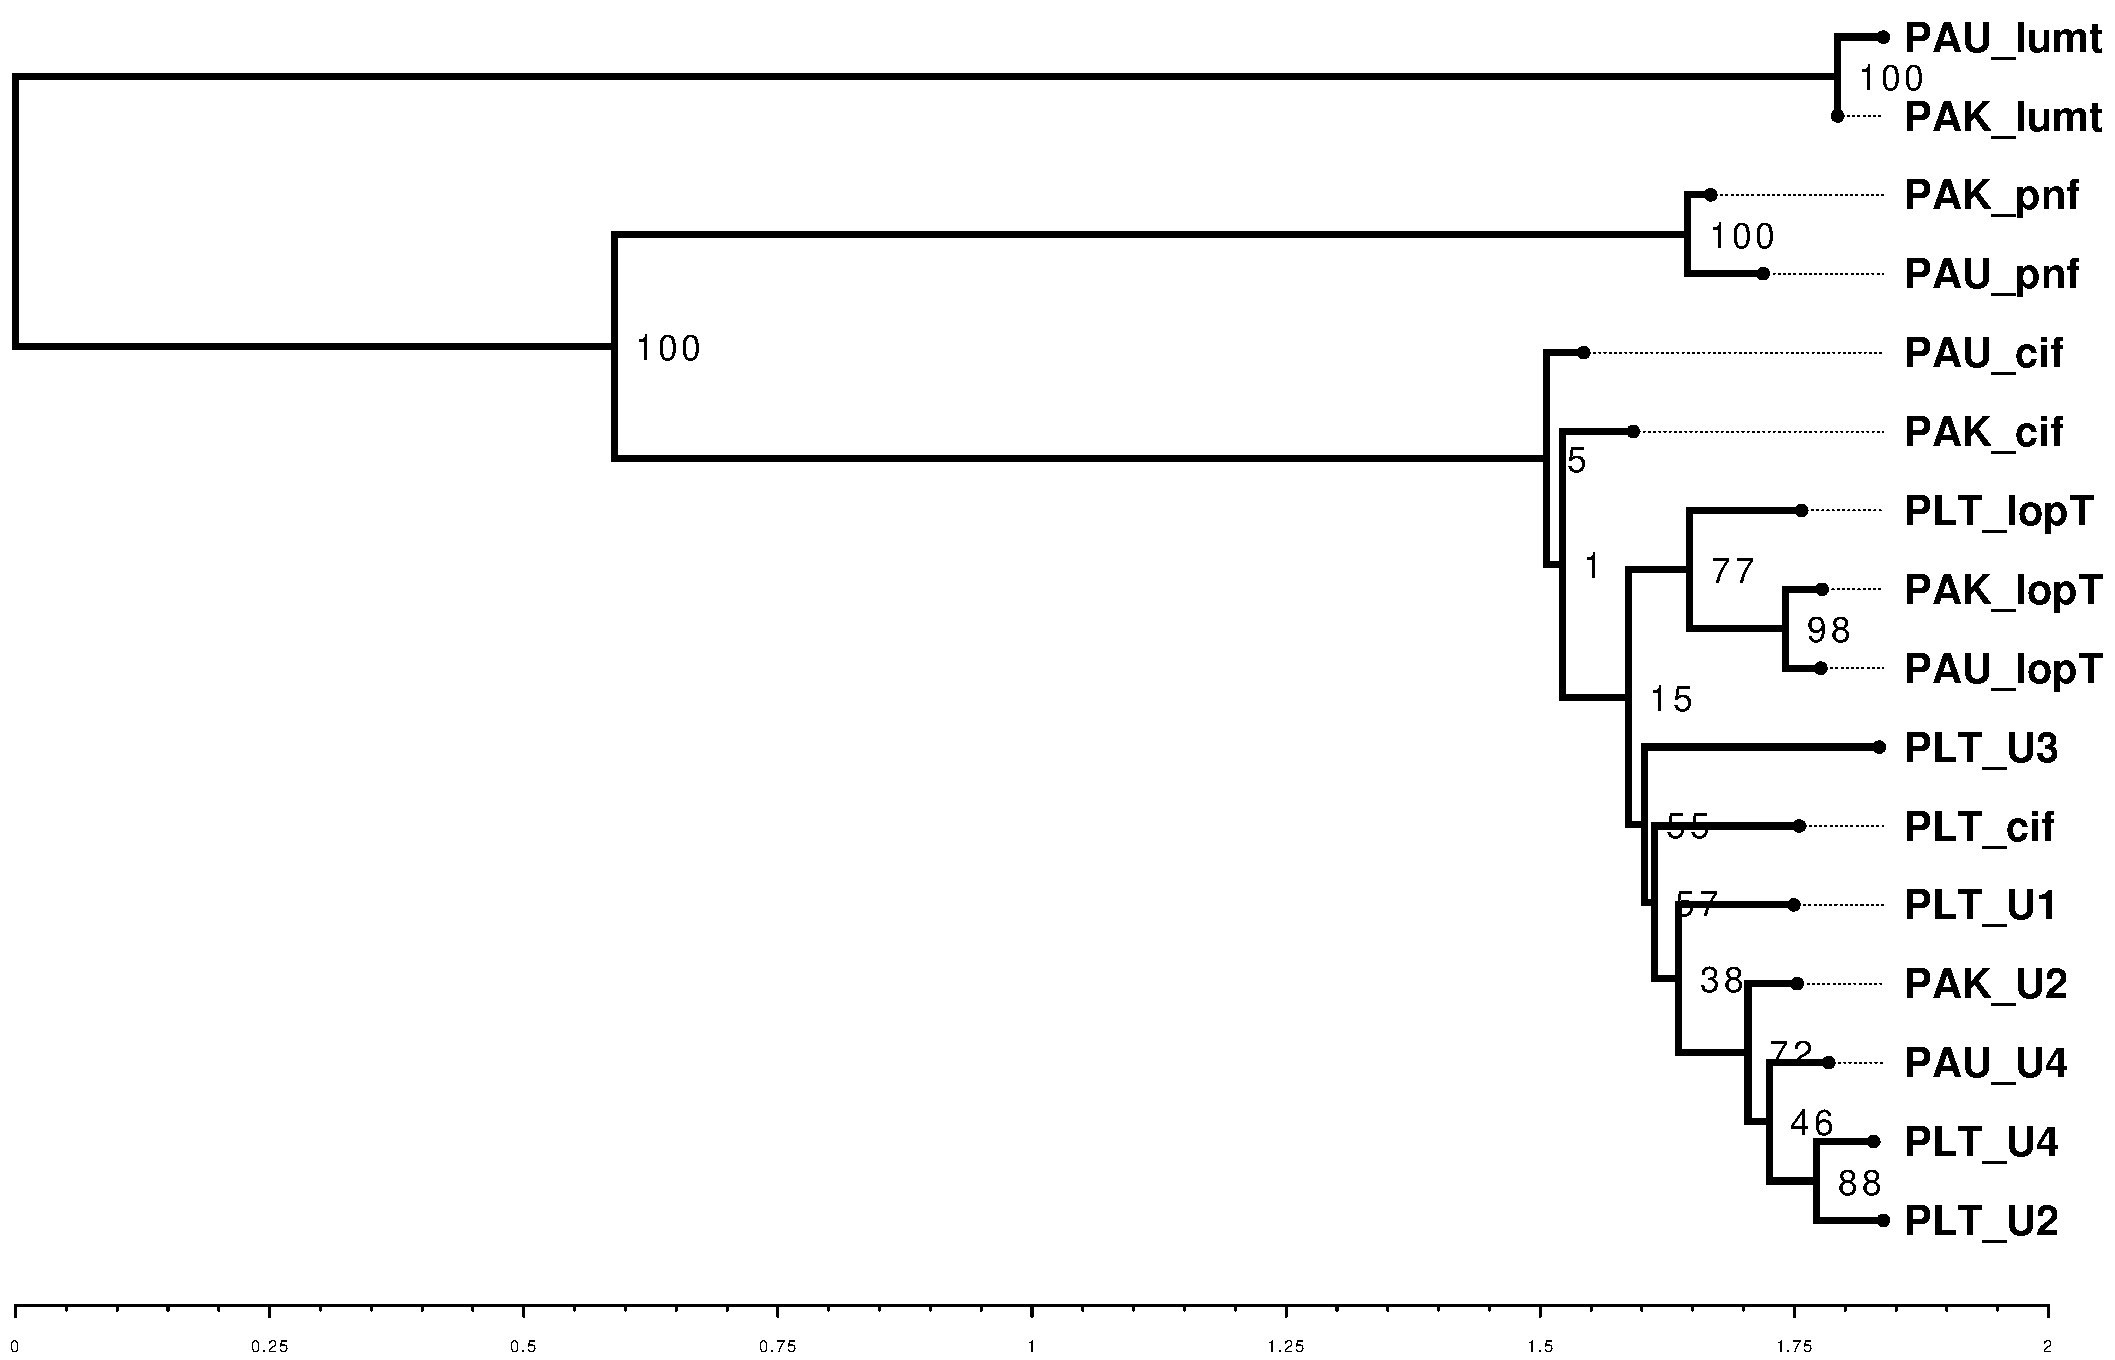
\includegraphics[width=0.95\textwidth]{/Users/joehealey/Documents/Warwick/PhD/Thesis/chapters/chapter4/img/PVC10.pdf}
	\captionsetup{singlelinecheck=off, justification=justified, font=footnotesize, aboveskip=19pt}
	\caption[Gene tree for the tenth PVC locus]{\textsc{\normalsize Maximum-likelihood tree of the locus position (PVC10) from each operon.}}
	\label{pvc10tree}
\end{figure}

\newpage
\begin{figure}[h!]
	\centering
	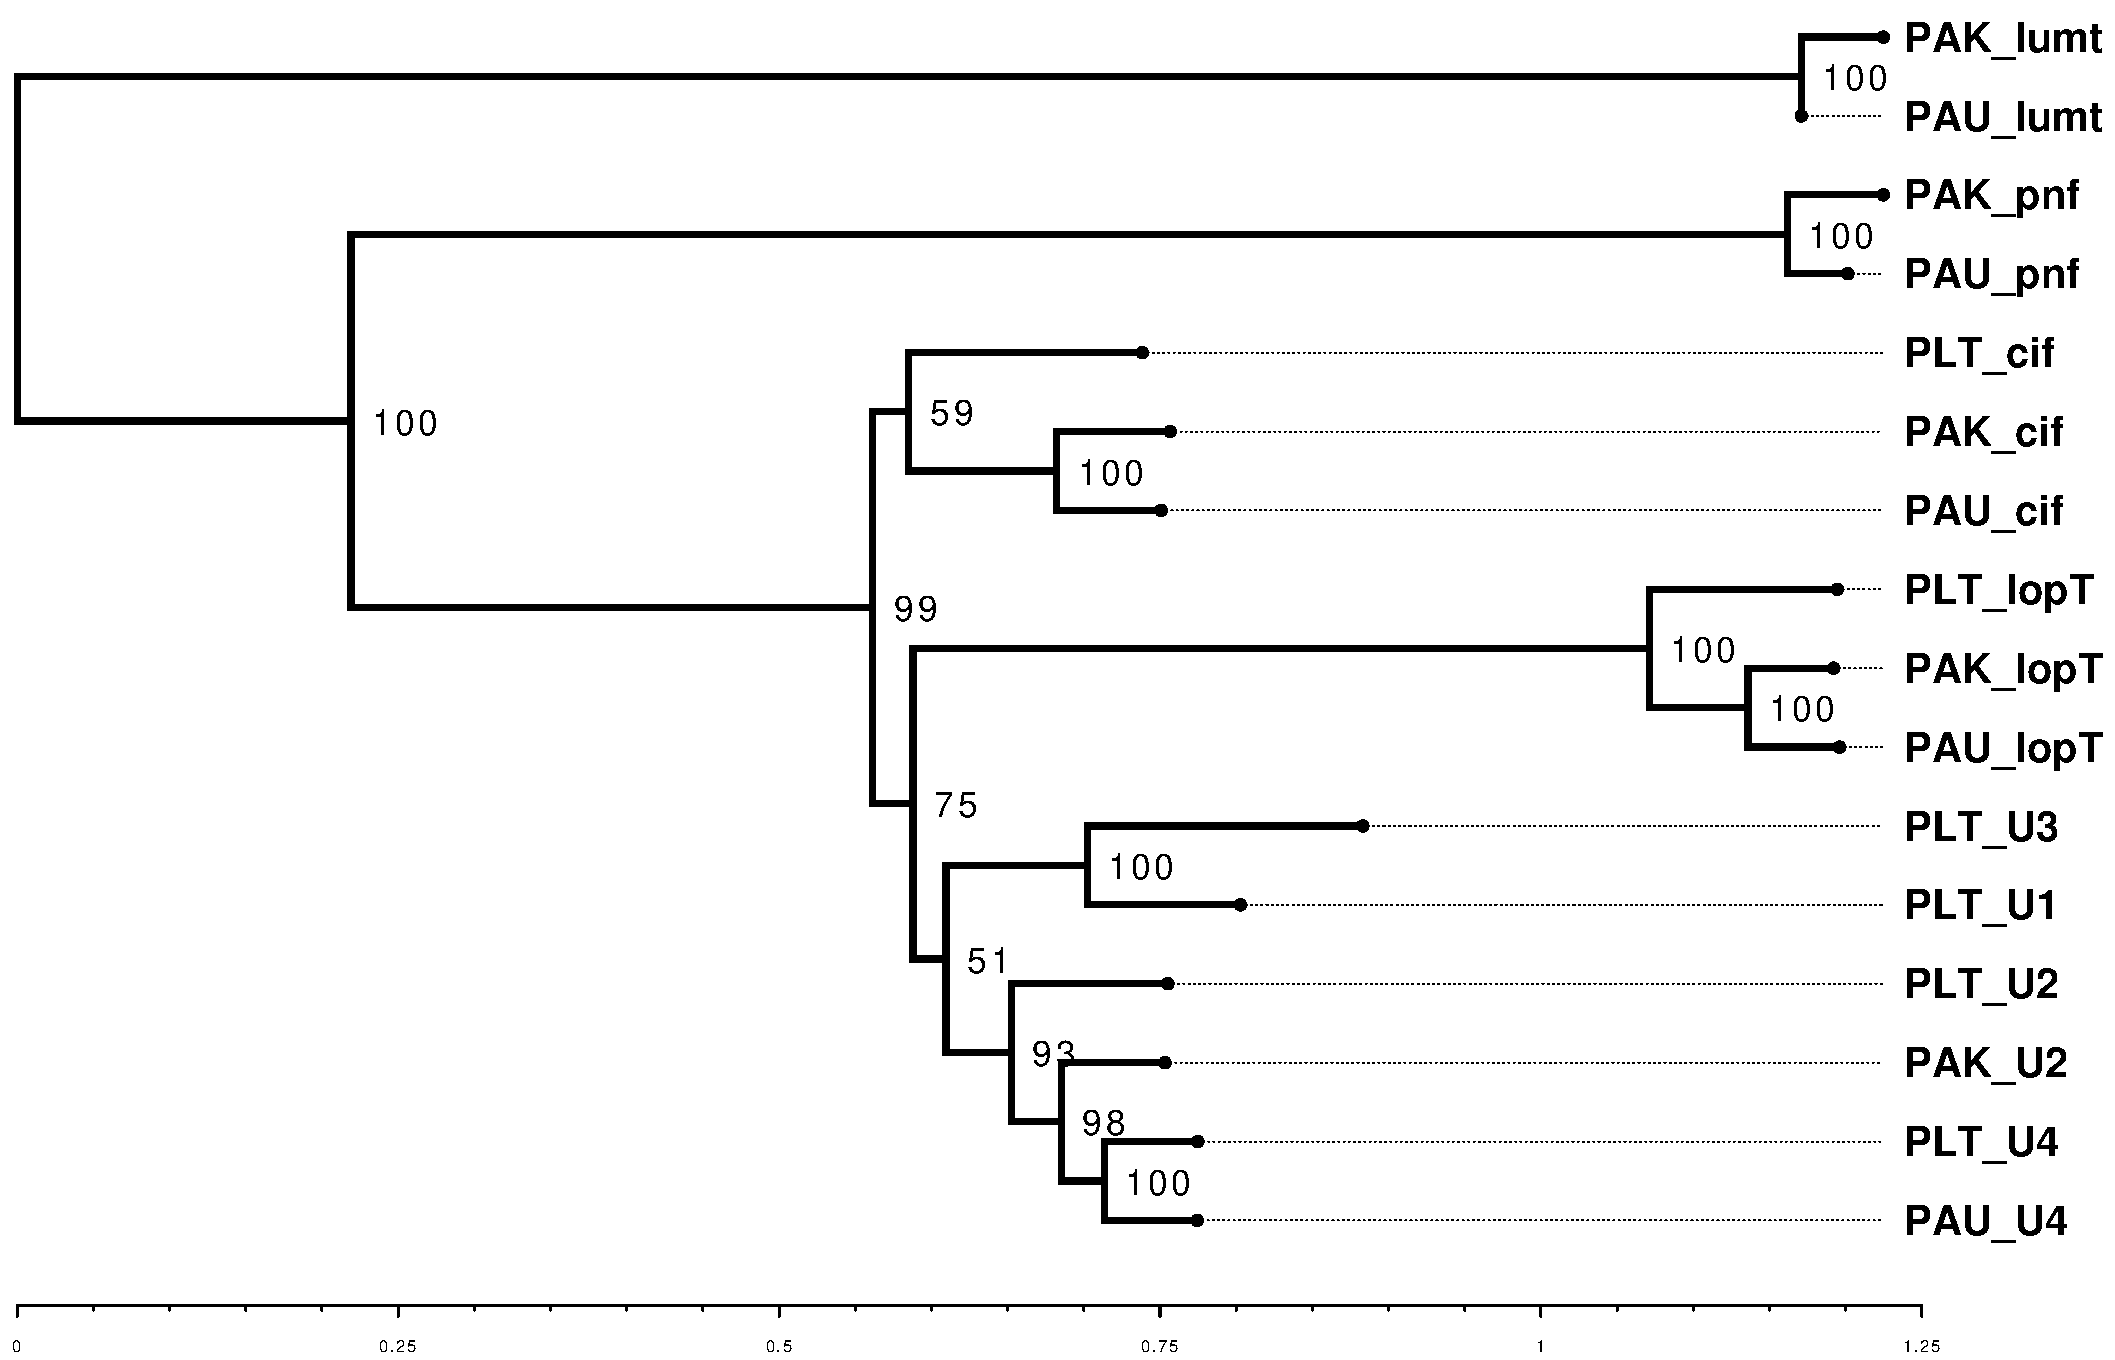
\includegraphics[width=0.95\textwidth]{/Users/joehealey/Documents/Warwick/PhD/Thesis/chapters/chapter4/img/PVC11.pdf}
	\captionsetup{singlelinecheck=off, justification=justified, font=footnotesize, aboveskip=19pt}
	\caption[Gene tree for the eleventh PVC locus]{\textsc{\normalsize Maximum-likelihood tree of the locus position (PVC11) from each operon.}}
	\label{pvc11tree}
\end{figure}
\hfill
\begin{figure}[h!]
	\centering
	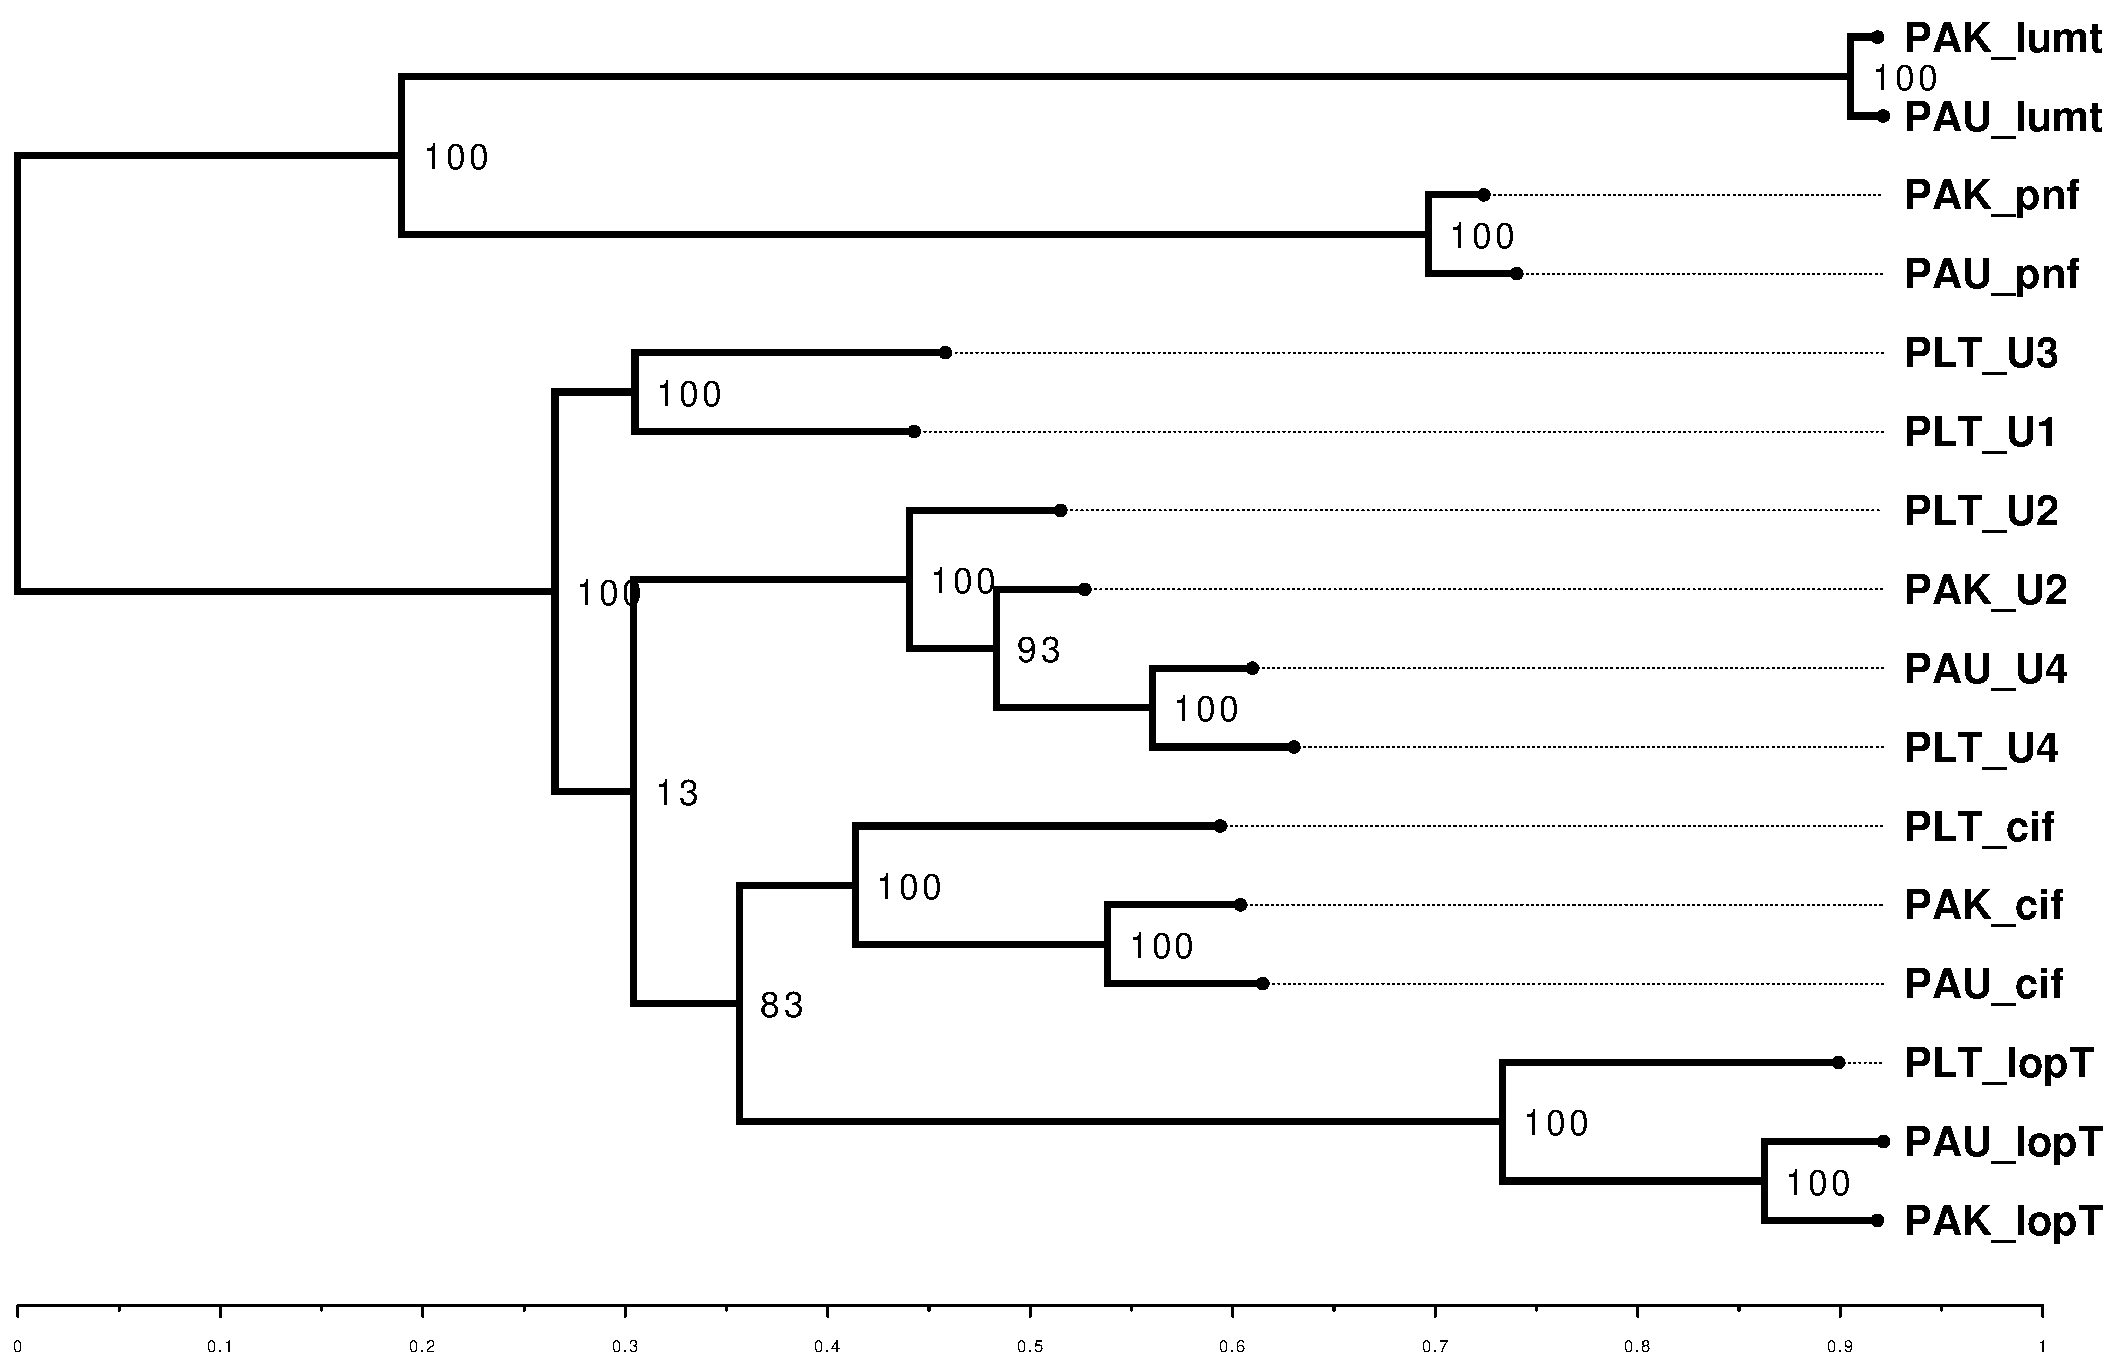
\includegraphics[width=0.95\textwidth]{/Users/joehealey/Documents/Warwick/PhD/Thesis/chapters/chapter4/img/PVC12.pdf}
	\captionsetup{singlelinecheck=off, justification=justified, font=footnotesize, aboveskip=19pt}
	\caption[Gene tree for the twelfth PVC locus]{\textsc{\normalsize Maximum-likelihood tree of the locus position (PVC12) from each operon.}}
	\label{pvc12tree}
\end{figure}

\newpage
\begin{figure}[h!]
	\centering
	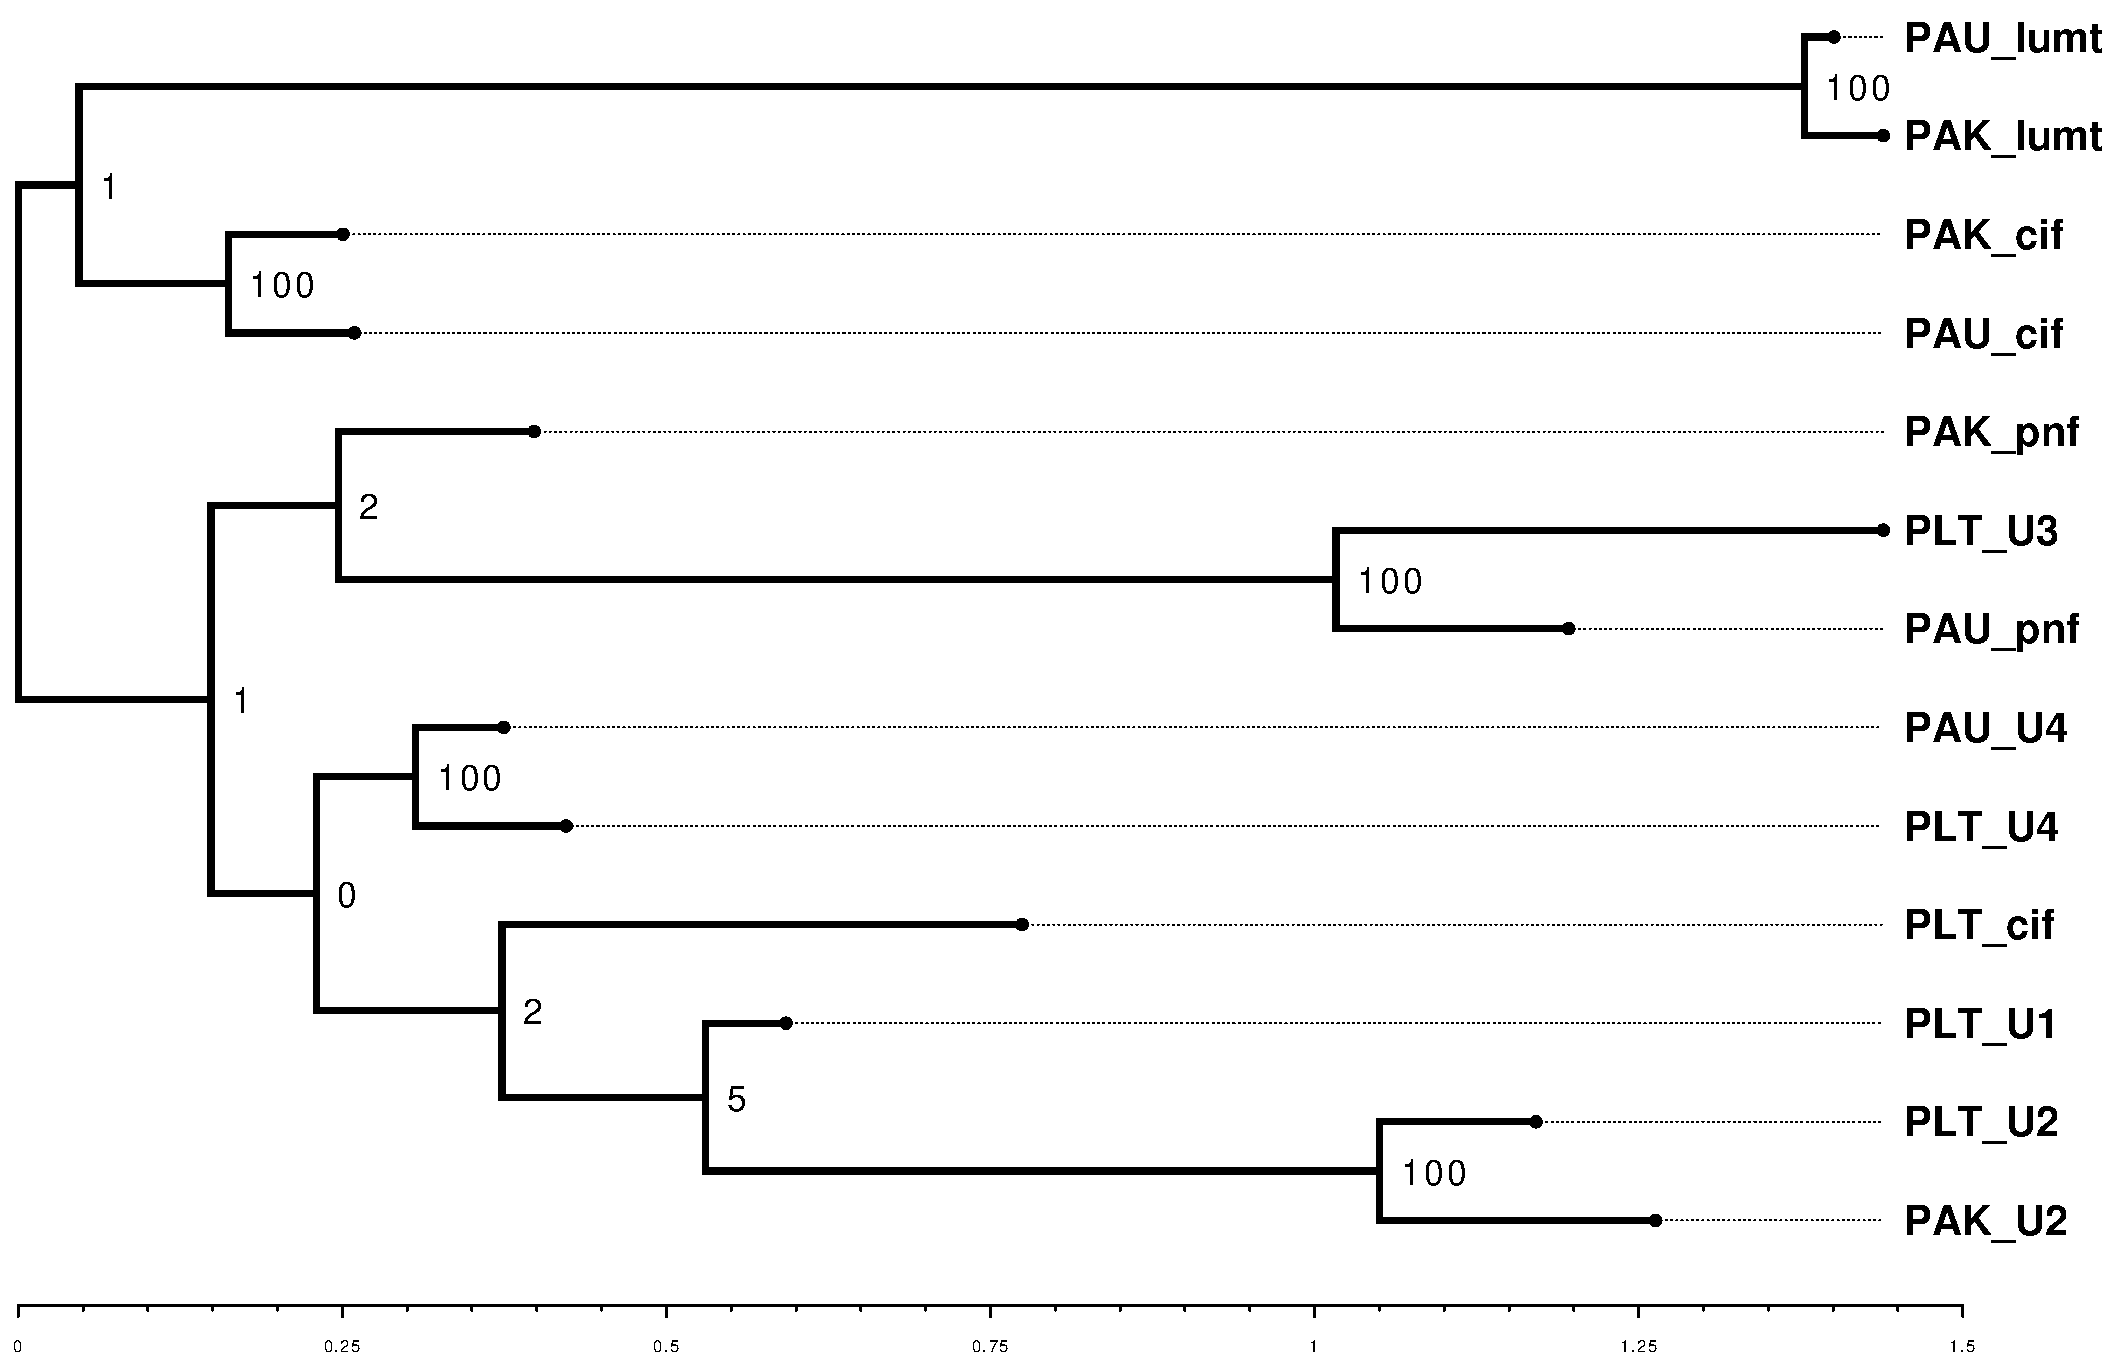
\includegraphics[width=0.95\textwidth]{/Users/joehealey/Documents/Warwick/PhD/Thesis/chapters/chapter4/img/PVC13.pdf}
	\captionsetup{singlelinecheck=off, justification=justified, font=footnotesize, aboveskip=19pt}
	\caption[Gene tree for the thirteenth PVC locus]{\textsc{\normalsize Maximum-likelihood tree of the locus position (PVC13) from each operon.}}
	\label{pvc13tree}
\end{figure}
\hfill
\begin{figure}[h!]
	\centering
	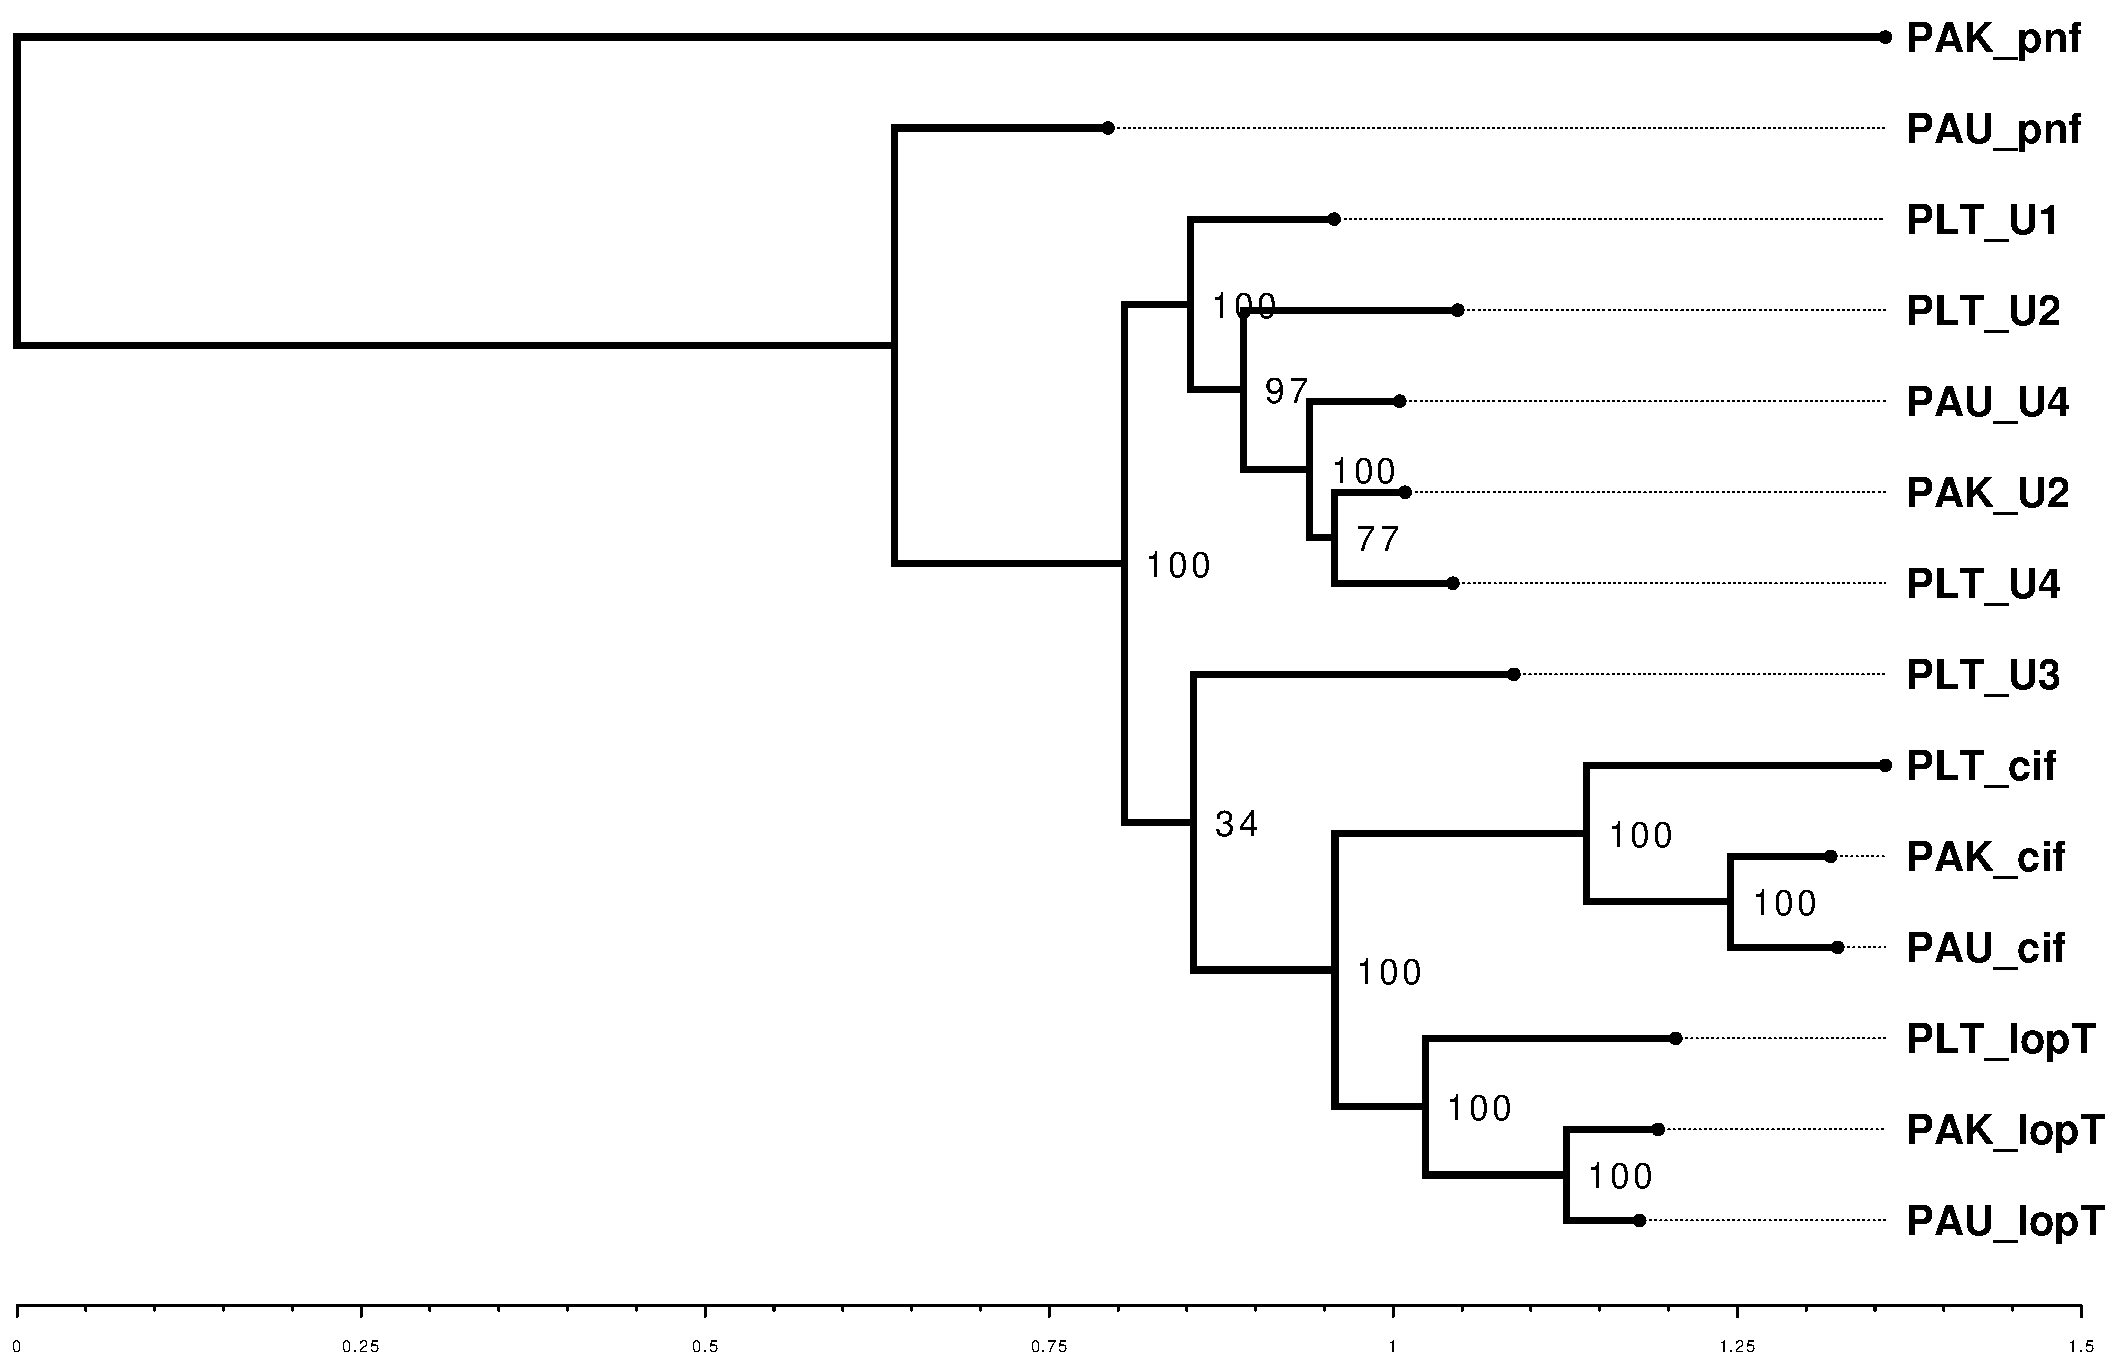
\includegraphics[width=0.95\textwidth]{/Users/joehealey/Documents/Warwick/PhD/Thesis/chapters/chapter4/img/PVC14.pdf}
	\captionsetup{singlelinecheck=off, justification=justified, font=footnotesize, aboveskip=19pt}
	\caption[Gene tree for the fourteenth PVC locus]{\textsc{\normalsize Maximum-likelihood tree of the locus position (PVC14) from each operon.}}
	\label{pvc14tree}
\end{figure}

\newpage
\begin{figure}[h!]
	\centering
	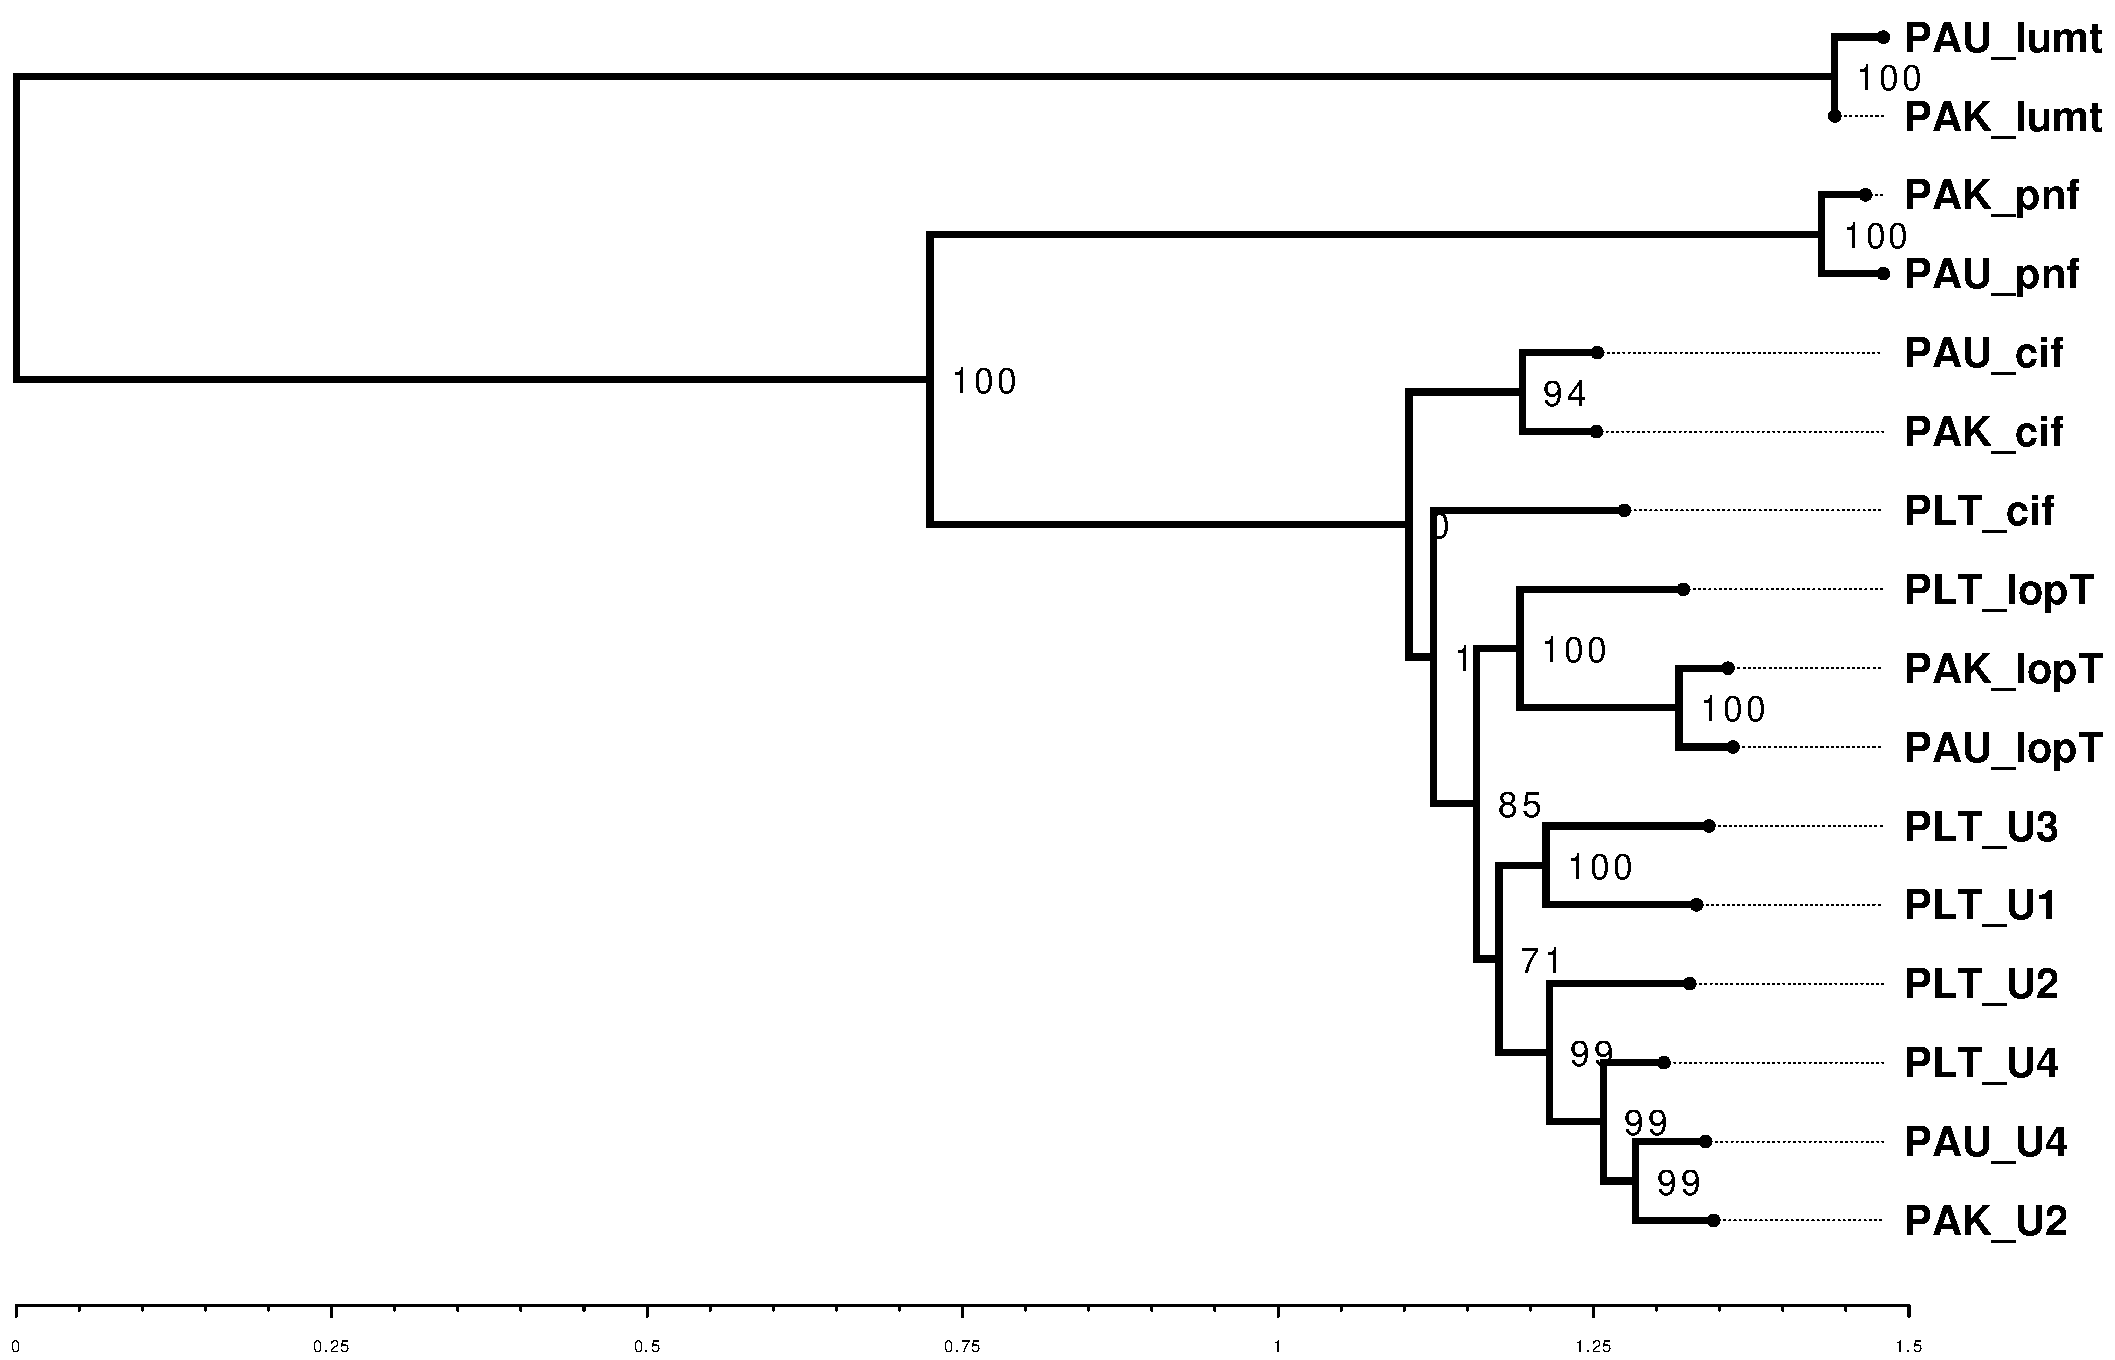
\includegraphics[width=0.95\textwidth]{/Users/joehealey/Documents/Warwick/PhD/Thesis/chapters/chapter4/img/PVC15.pdf}
	\captionsetup{singlelinecheck=off, justification=justified, font=footnotesize, aboveskip=19pt}
	\caption[Gene tree for the fifteenth PVC locus]{\textsc{\normalsize Maximum-likelihood tree of the locus position (PVC15) from each operon.}}
	\label{pvc15tree}
\end{figure}
\hfill
\begin{figure}[h!]
	\centering
	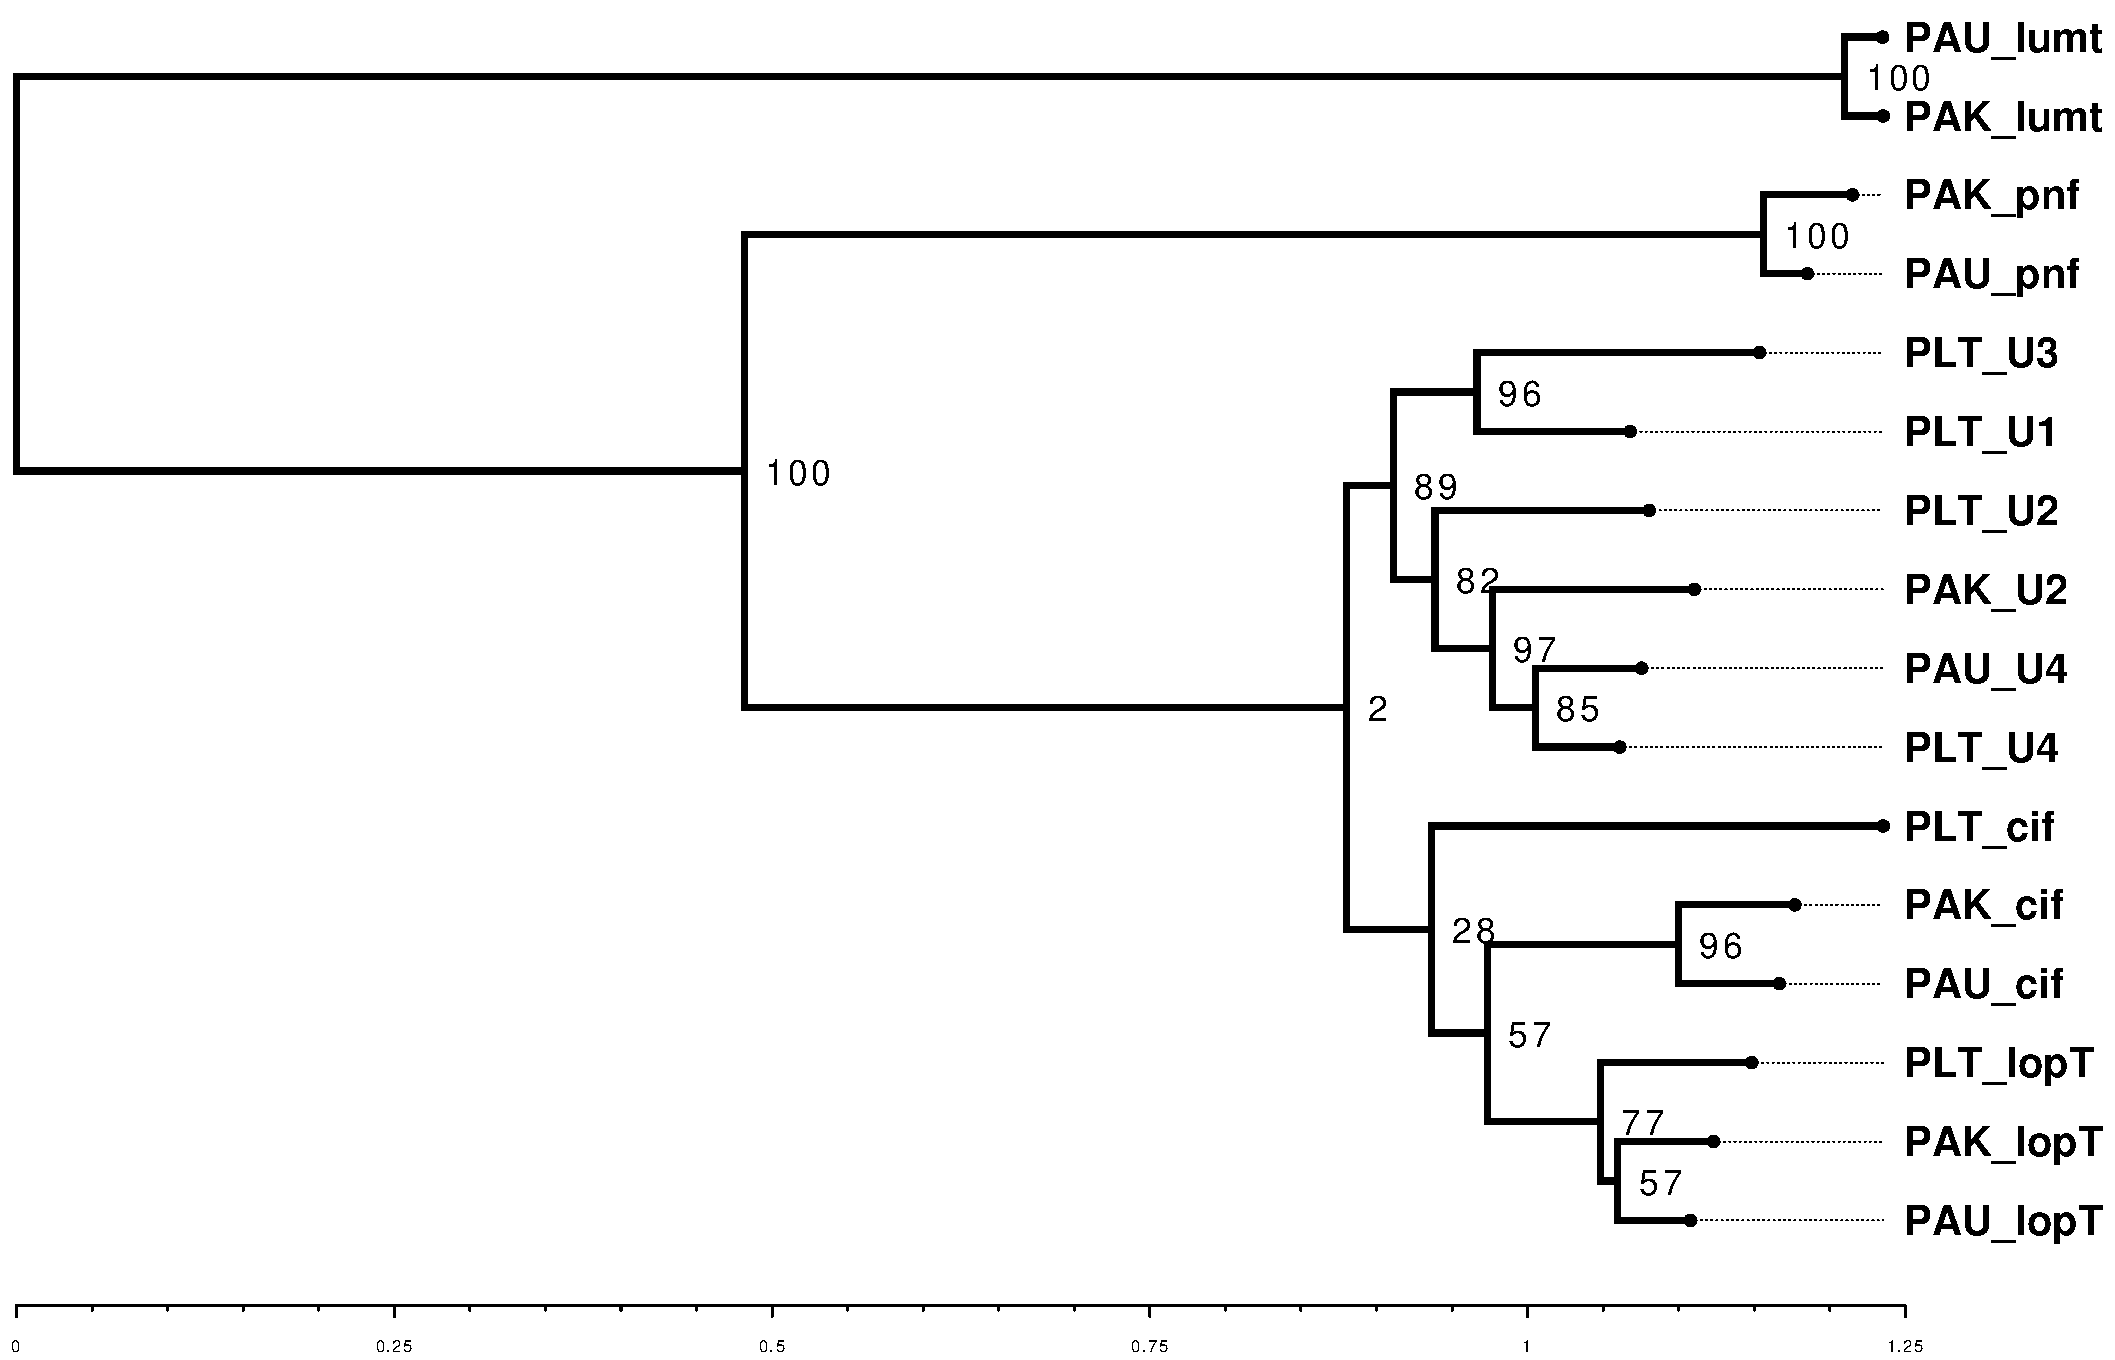
\includegraphics[width=0.95\textwidth]{/Users/joehealey/Documents/Warwick/PhD/Thesis/chapters/chapter4/img/PVC16.pdf}
	\captionsetup{singlelinecheck=off, justification=justified, font=footnotesize, aboveskip=19pt}
	\caption[Gene tree for the sixteenth PVC locus]{\textsc{\normalsize Maximum-likelihood tree of the locus position (PVC16) from each operon.}}
	\label{pvc16tree}
\end{figure}

\newpage

\subsection{Consensus Tree Inference via ASTRAL-II}
The penultimate step of the congruency work flow was to infer the consensus tree from just the sequences within the PVC operons. By doing so, we can determine which patterns of evolution from genes within the operon most and least closely follow the known species phylogeny during the congruency analysis. \vref{consensustree} shows the inferred phylogeny output by ASTRAL-II \citep{Mirarab2015}. ASTRAL was run with the bootstrap gene trees from RAxML. The software arbitrarily selects a taxa to root from, in this case PLT\_U2. The tree is otherwise depicted in decreasing node order for clarity and consistency with the gene trees.

\vspace{1cm}
\begin{figure}[h!]
	\centering
	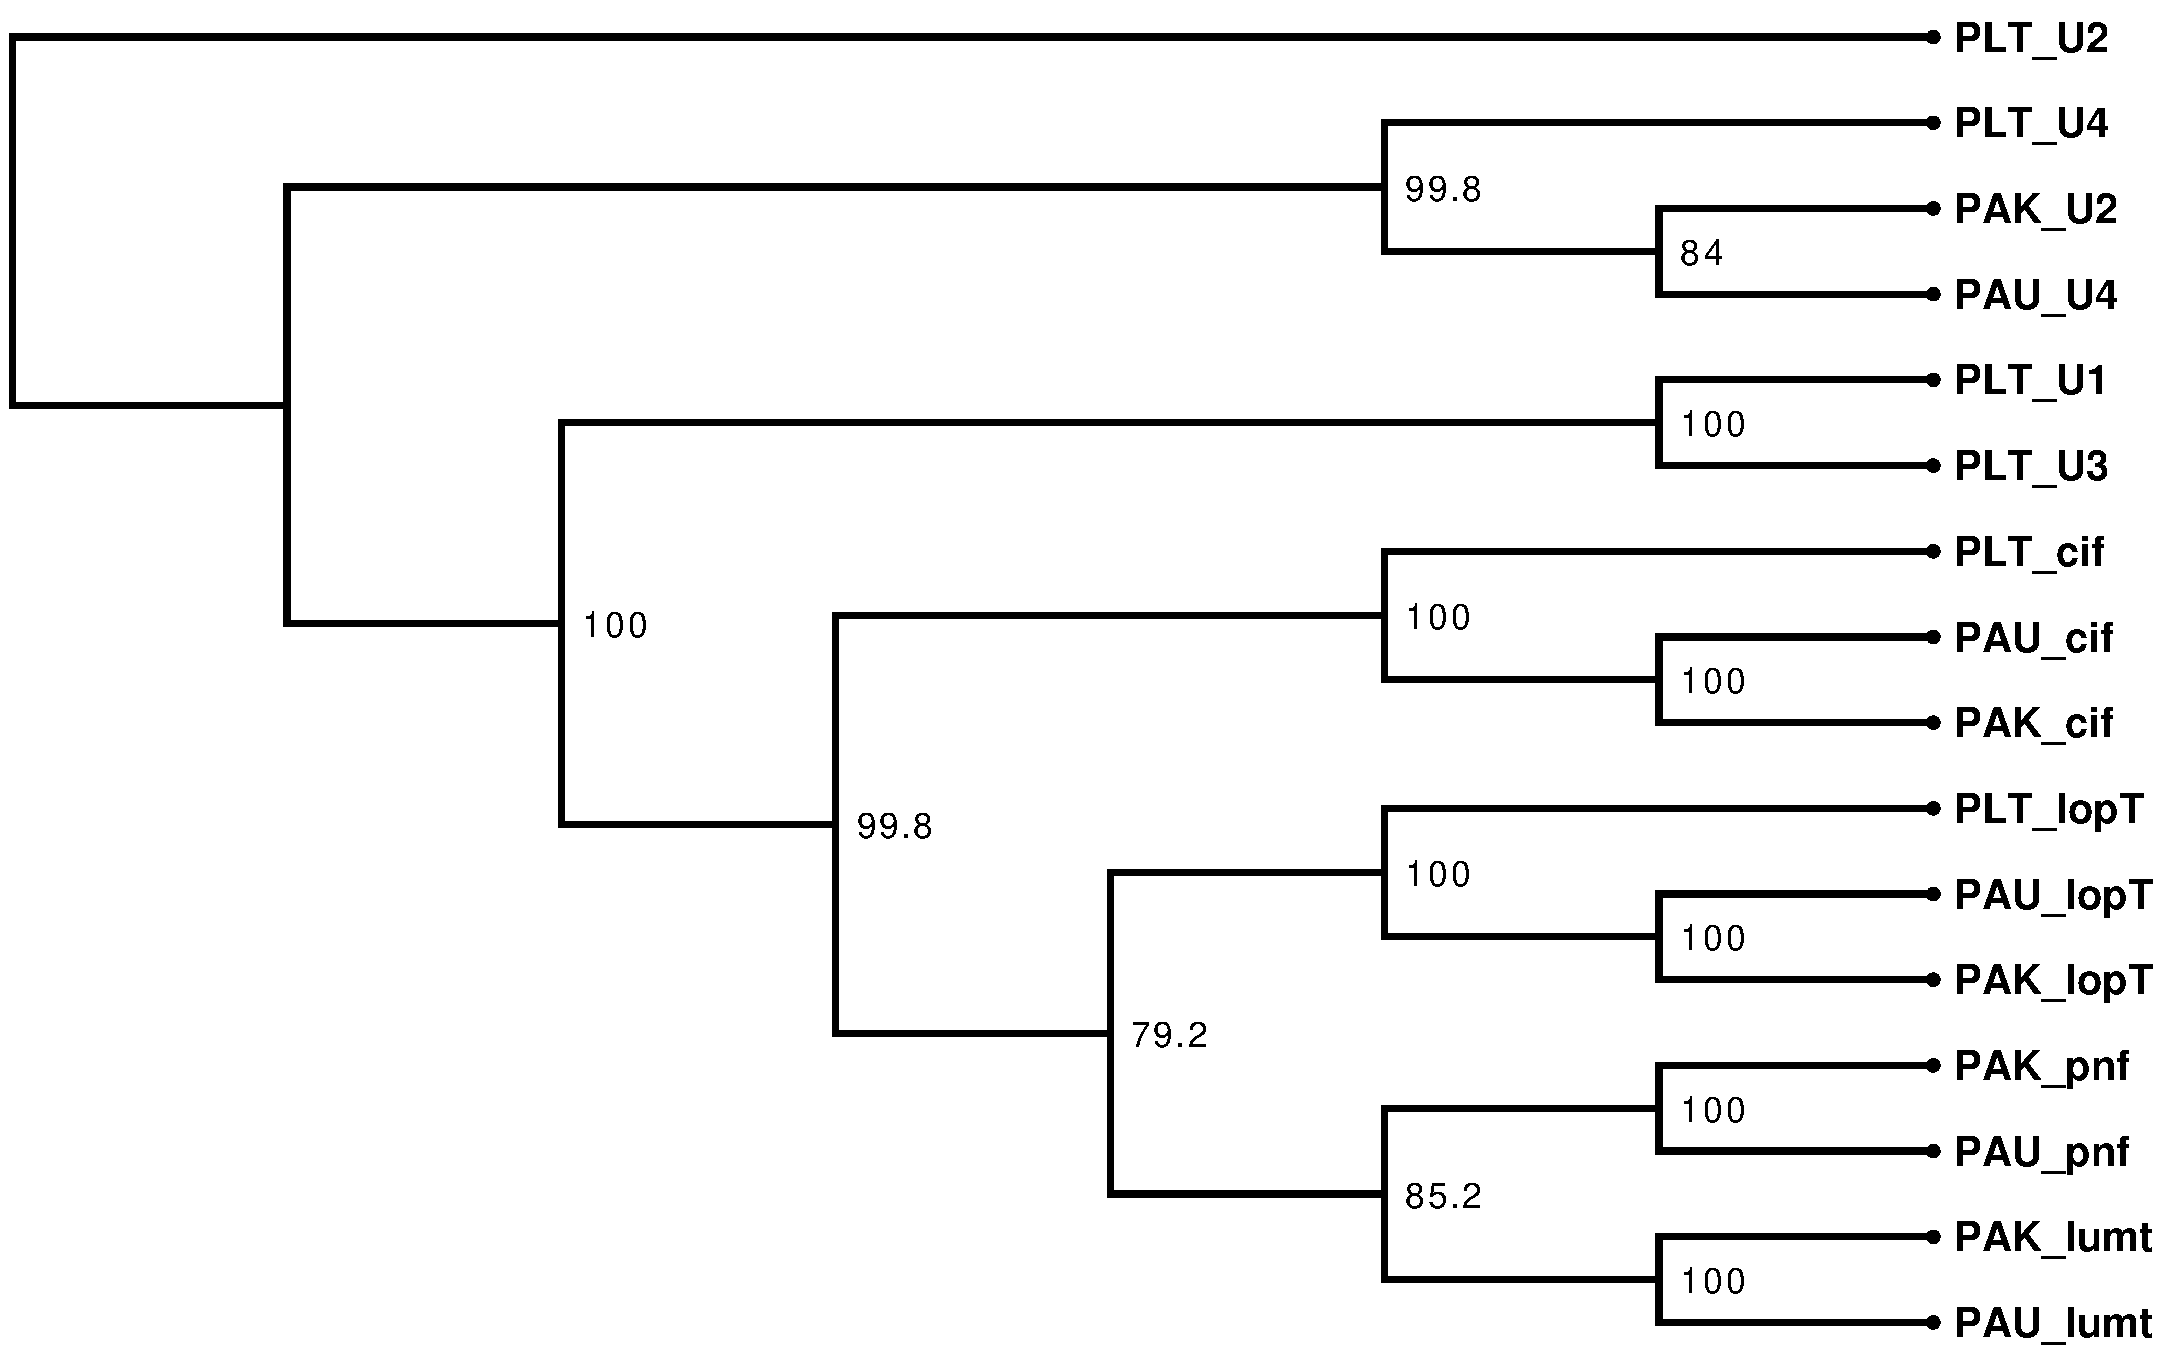
\includegraphics[width=0.95\textwidth]{/Users/joehealey/Documents/Warwick/PhD/Thesis/chapters/chapter4/img/PVC17.pdf}
	\captionsetup{singlelinecheck=off, justification=justified, font=footnotesize, aboveskip=19pt}
	\caption[Consensus Tree]{The inferred consensus tree from the genetrees PVC1-16. Branch lengths are arbitrary for this tree and therefore it has been depicted as an cladogram with no scale.}
	\label{consensustree}
\end{figure}

The tree shows well supported branches for all splits, and consistently clusters orthologous operons together (e.g. all Pnfs, Cifs etc.).


\subsection{Congruency Analysis}
	With each gene tree output from RAxML and the 17th tree as the inferred tree from ASTRAL-II, the pairwise congruency between all trees was calculated. Evaluation of congruency metrics ultimately means one is able to put a single number on to a subject tree with respect to a reference, to say how similar the 2 trees are - and ultimately whether they follow the same evolutionary pattern.
	
\subsubsection{Adjusted Wallace Coefficient}
	Congruency was initially tested utilising a metric called the Adjusted Wallace Coefficient (AWC). The Wallace coefficient is one of many used in the study of clustering concordance, but has advantages over others such as the well known Rand metric \citep{Rand1971}, in that it has a `directional component' \citep{Wallace1983}. The Wallace coefficient can be thought of as saying ``what is the probability that some data is classified together in test B, knowing that it also was in test A". Details of how the AWC is calculated can be found in \vref{methods}, and at the associated references.

\subsubsection{Normalised Robinson-Foulds}
	To address the issue of subjectivity in the previous clustering method, an unbiased although lower resolution technique was used to corroborate the trends - the topological transformation metric developed by Robinson and Foulds (``RF")\citep{Robinson1981}. The RF distance is useful specifically for unrooted trees such as these, since it makes no assumptions about any particular nodes/leaves, it simply calculates the minimum number of topological transformations required to make 2 trees maximally congruent.  Because of this, the RF metric is a symmetric one (transforming A = B, is an equivalent number of transforms to make B = A, but reversed with respect to one another). 
	
\begin{figure}[p]
\thisfloatpagestyle{IHA-fancy-style}
	\centering
\begin{subfigure}[H]{\textwidth}
	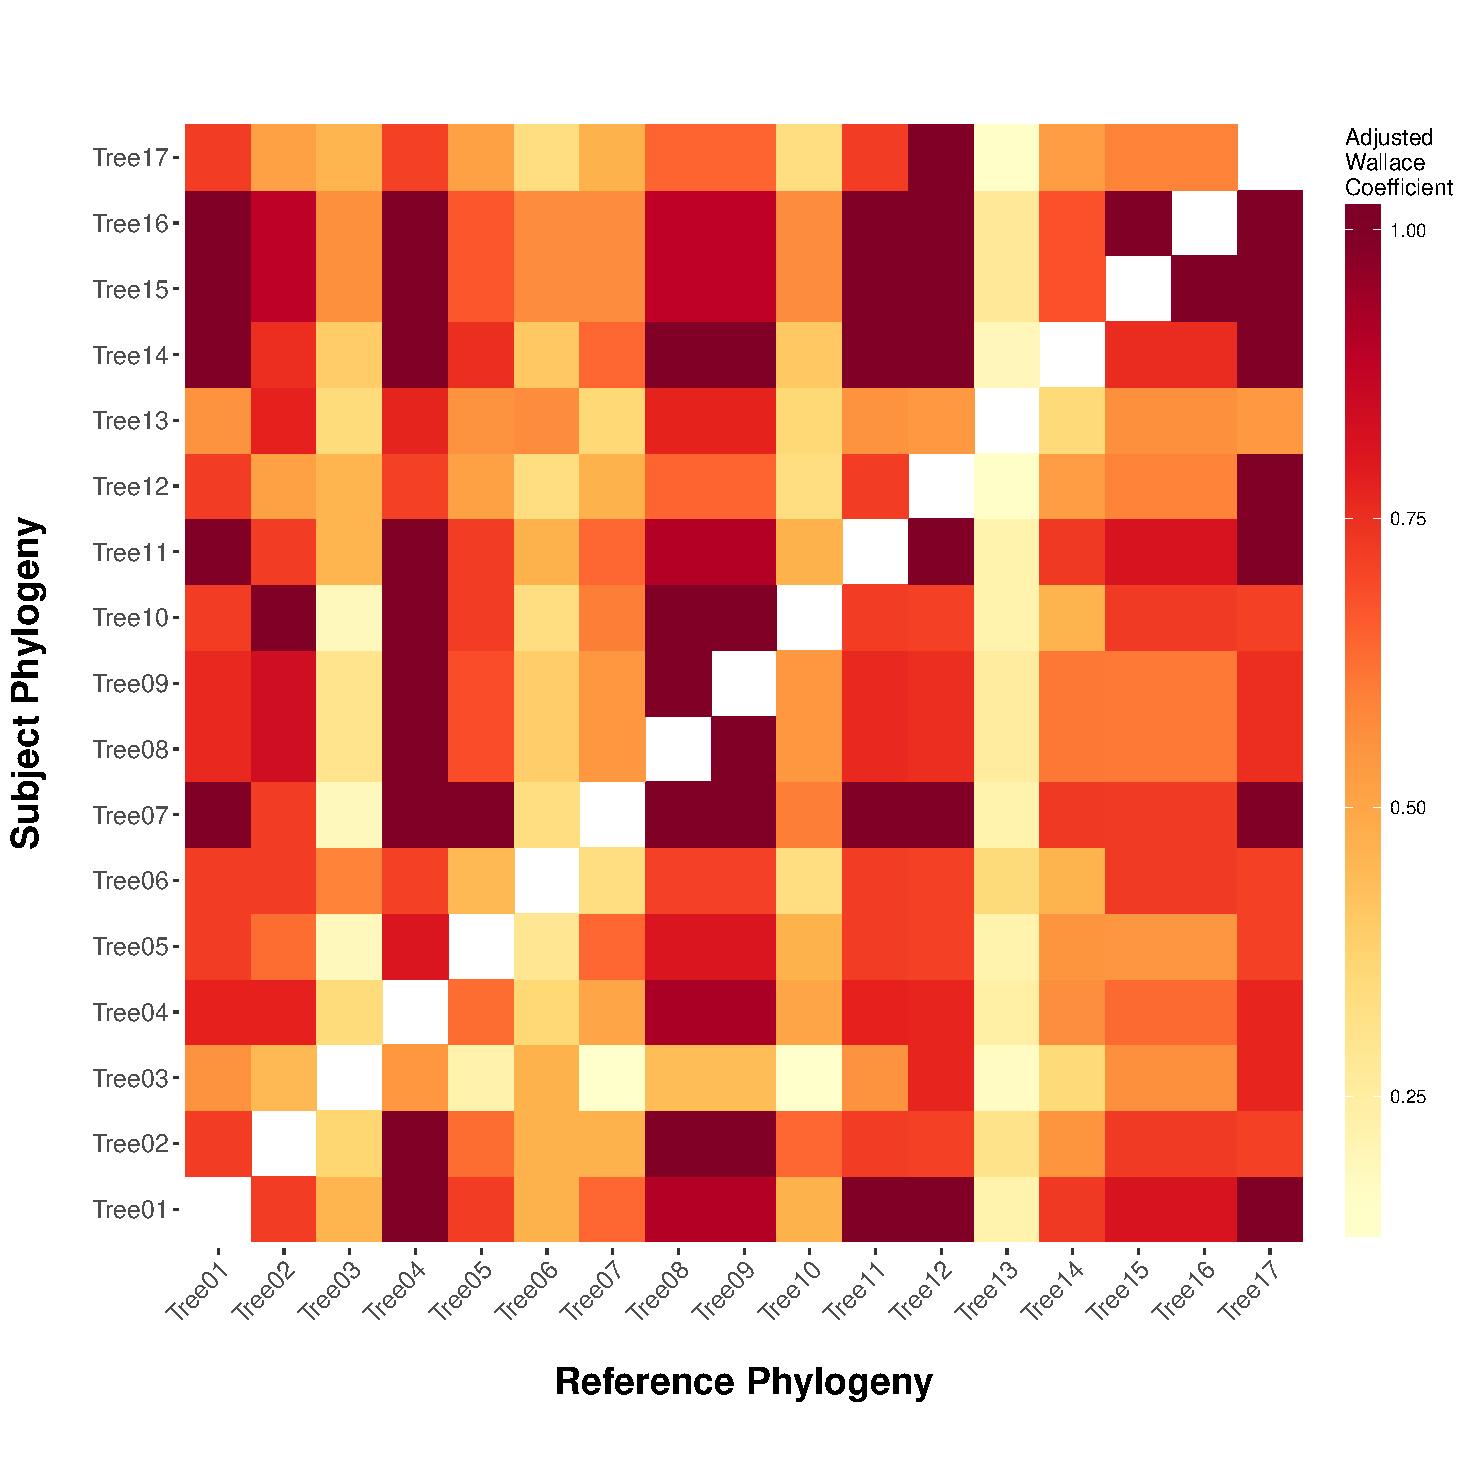
\includegraphics[width=\textwidth, trim={0 20 0 0}, clip]{/Users/joehealey/Documents/Warwick/PhD/Thesis/chapters/chapter4/img/ADJW.pdf}
\end{subfigure}
\begin{subfigure}[H]{\textwidth}
\footnotesize
\begin{tabularx}{1.01\textwidth}{CCCCCCCCCCCCCCCCC }
\hiderowcolors

\rotatebox{45}{Tree01} & \rotatebox{45}{Tree02} & \rotatebox{45}{Tree03} & \rotatebox{45}{Tree04} & \rotatebox{45}{Tree05} & \rotatebox{45}{Tree06} & \rotatebox{45}{Tree07} & \rotatebox{45}{Tree08} & \rotatebox{45}{Tree09} & \rotatebox{45}{Tree10} & \rotatebox{45}{Tree11} & \rotatebox{45}{Tree12} & \rotatebox{45}{Tree13} & \rotatebox{45}{Tree14} & \rotatebox{45}{Tree15} & \rotatebox{45}{Tree16} & \rotatebox{45}{Tree17}  \\
\cmidrule{1-17}
\multicolumn{17}{c}{Congruency Sums (Reference vs Subject) ($\mathrm{ADW}_{A\rightarrow B} $)} \\[0.2ex]
\cmidrule{1-17}\\[-2ex]
12.74 & 11.75 & 6.13 & 14.26 & 10.12 & 6.71 & 8.11 & 13.53 & 13.53 & 7.25 & 12.74 & 13.43 & 3.67 & 9.11 & 11.01 & 11.01 & 13.43 \\[0.5ex]
\cmidrule{1-17}
\multicolumn{17}{c}{Congruency Sums (Subject vs Reference) ($\mathrm{ADW}_{B\rightarrow A} $)}\\[0.1ex]
\cmidrule{1-17}\\[-2ex]
11.86 & 10.74 & 7.12 & 10.12 & 9.36 & 9.69 & 12.23 & 10.41 & 10.41 & 10.83 & 11.86 & 8.91 & 8.95 & 12.05 & 12.55 & 12.55  & 8.91  \\

\end{tabularx}
\end{subfigure}

	\captionsetup{singlelinecheck=off, justification=justified, font=footnotesize, aboveskip=20pt}
	\caption[All pairwise comparisons of congruency as measured by the Adjusted Wallace Coefficient (AWC)]{\textsc{\normalsize Visualised congruency between trees (Ajdusted Wallace Coefficient).} \vspace{0.1cm} \newline All pairwise comparisons of congruency as measured by the Adjusted Wallace Coefficient. The darker the colour, the better the congruency is. Adjusted Wallace Coefficients of 1 indicate good agreement. The cumulative summed congruency for each locus is displayed below, to quickly show numerically the most and least congruent. There are 2 sets of values for the row and column sums due to the asymmetry of the Adjusted Wallace Coefficient.}

	\label{ADWheatmap}
\end{figure}
	
\begin{figure}[p]
\thisfloatpagestyle{IHA-fancy-style}
	\centering
\begin{subfigure}[H]{\textwidth}
	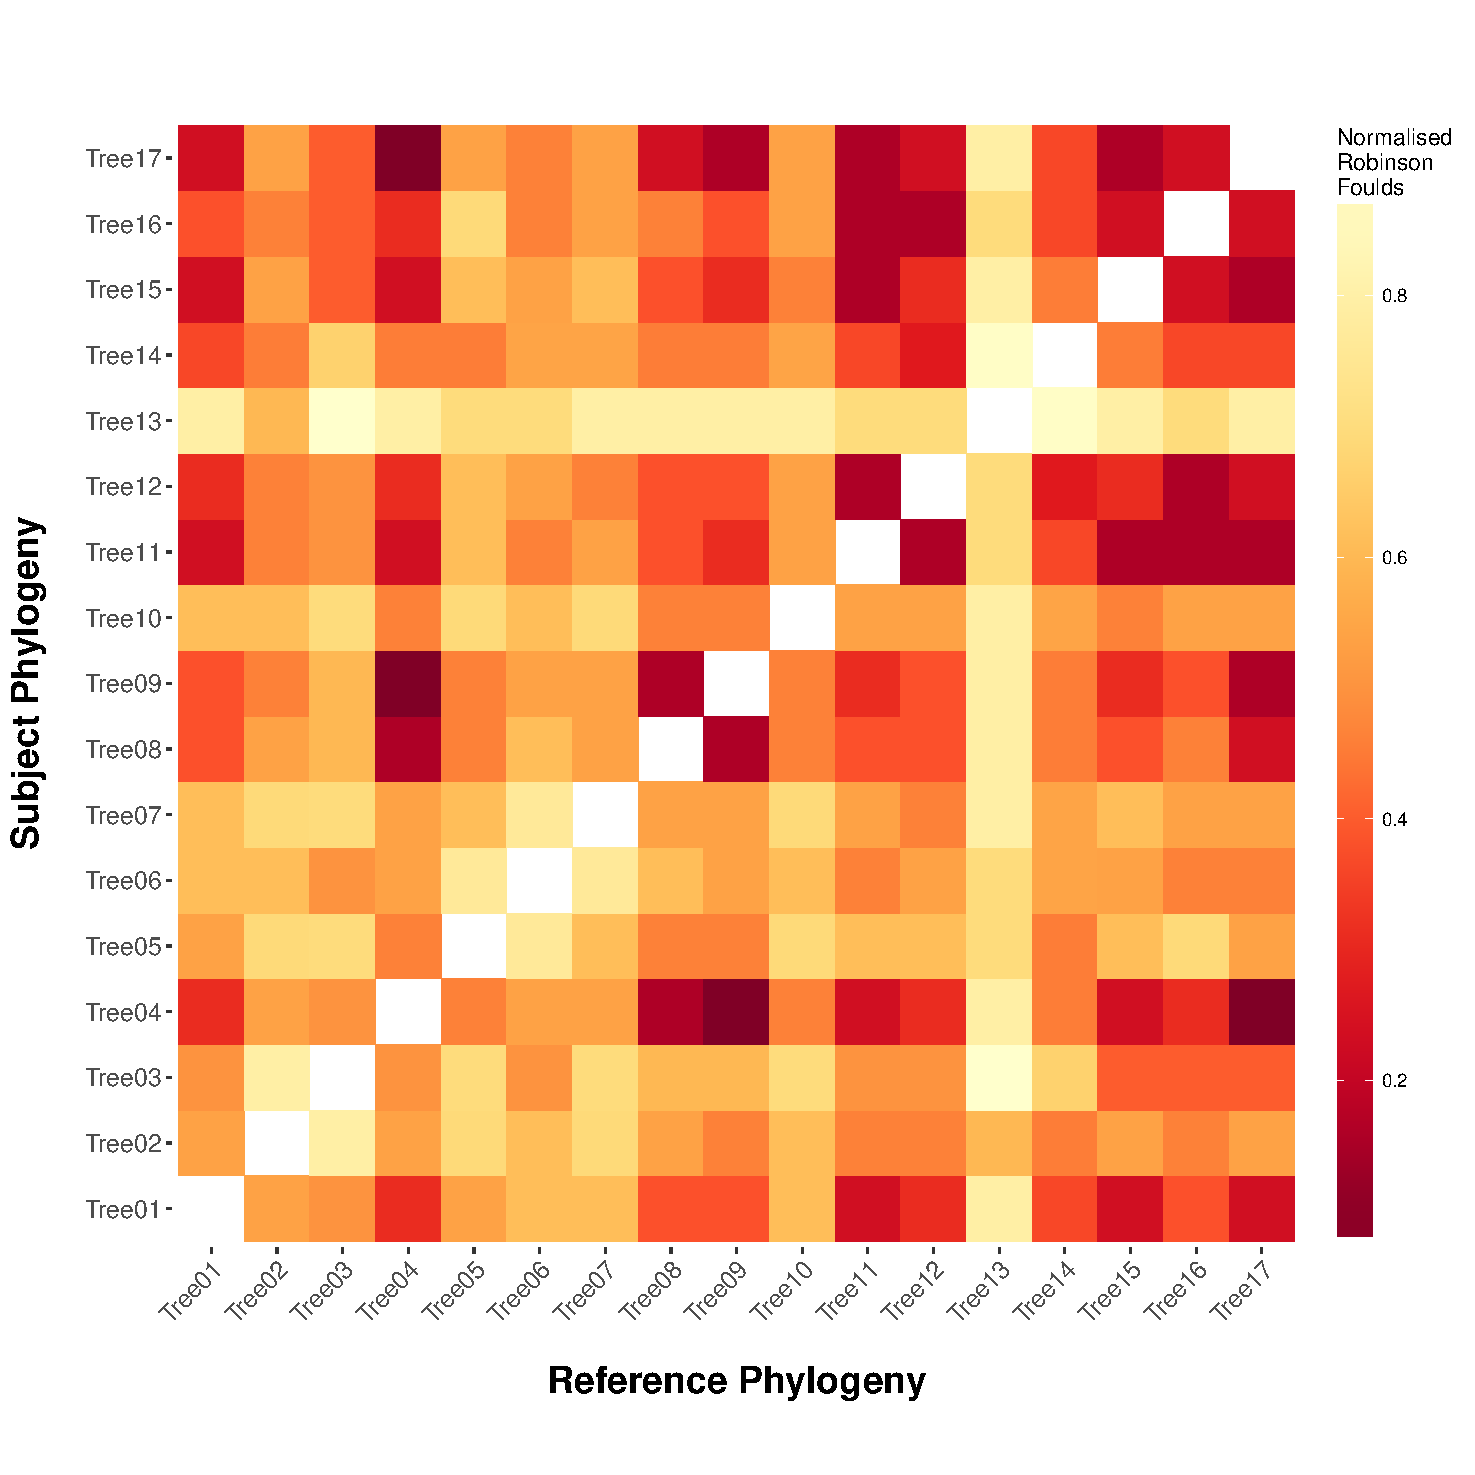
\includegraphics[width=\textwidth]{/Users/joehealey/Documents/Warwick/PhD/Thesis/chapters/chapter4/img/nRF.pdf}
\end{subfigure}
\begin{subfigure}[H]{\textwidth}
\footnotesize
\begin{tabularx}{1.01\textwidth}{CCCCCCCCCCCCCCCCC }
\hiderowcolors

\rotatebox{45}{Tree01} & \rotatebox{45}{Tree02} & \rotatebox{45}{Tree03} & \rotatebox{45}{Tree04} & \rotatebox{45}{Tree05} & \rotatebox{45}{Tree06} & \rotatebox{45}{Tree07} & \rotatebox{45}{Tree08} & \rotatebox{45}{Tree09} & \rotatebox{45}{Tree10} & \rotatebox{45}{Tree11} & \rotatebox{45}{Tree12} & \rotatebox{45}{Tree13} & \rotatebox{45}{Tree14} & \rotatebox{45}{Tree15} & \rotatebox{45}{Tree16} & \rotatebox{45}{Tree17}  \\
\cmidrule{1-17}
\multicolumn{17}{c}{Congruency Sums} \\[0.2ex]
\cmidrule{1-17}\\[-2ex]
7.05 &  9.01 &  9.36 &  5.99 &  9.62  & 9.28 &  9.74 &  7.01 &  6.47 &  9.28 &  5.95 &  6.32 & 12.26 &  7.63 &  6.42 &  6.46 &  5.64 \\[0.5ex]
\end{tabularx}
\end{subfigure}
	\captionsetup{singlelinecheck=off, justification=justified, font=footnotesize, aboveskip=20pt}
	\caption[All pairwise comparisons of congruency as measured by the Normalised Robinson-Foulds metric (nRF)]{\textsc{\normalsize Visualised congruency between trees (Robinson-Foulds).} \vspace{0.1cm} \newline All pairwise comparisons of congruency as measured by the Normalised Robinson-Foulds metric (nRF). The closer the nRF is to 0 (as depicted by the darker colours in this heatmap), the better the congruency is. Note that the metric scale is reversed relative to the previous heatmap, but the colourscale has been inverted to maintain colour consistency (i.e. darker colours are more congruent for both heatmaps). The cumulative summed congruency for each locus is displayed below, to quickly show numerically the most and least congruent.}
	\label{nRFheatmap}
	\end{figure}
 
\newpage

\section{Discussion}
The data for the congruency methods reveals several trends and unambiguously confirms hypotheses about PVC13, the putative phage tail-fibre like gene. Multiple sequence alignments (MSAs) for all the data generated here are given in \vref{bioinformatics_appendixs}, as they take up considerable space. 

Proceeding consecutively, PVCs 1 and 2, which comprise part of the inner and outer tube of the needle complex respectively, both score well in general for congruency. This is as expected; these proteins are present in every PVC, and are always the first 2 genes in the operon (with the exception of ``PVC0" that was discussed in \vref{clustering}). As can be seen from \vref{AAID}, PVC1 is generally quite well conserved, though some interesting gross architecture begins to emerge. It seems that the various ``Unit \#" operons, and ``LopT", cluster together quite neatly, but the remaining PVCs begin to segregate somewhat. This is potentially suggestive of the inner sheath adaptations the PVCs are undergoing to accommodate their cognate payloads. Since the exterior sheath serves essentially the same purpose in all the PVCs, regardless of their payload, it doesn't seem surprising that they almost all cluster considerably closer to one another, with short branch lengths and low bootstraps in places. The very obvious exception to this which is apparent in both the multiple sequence alignment (MSA) \vref{bioinformatics_appendix}, and the tree, is that the ``lumt" operons from both the \emph{P. asymbiotica} genomes vary enormously. These sequences align quite well locally to the other sequences, but contain many more residues versus the other sequences (though Kingscliff's ``lumt" gene has a truncated C-terminus). One hypothesis to explain this is that the additional residues form extra surface loops, potentially altering the target organisms' immune response to the complex, while maintaining the contractile functionality.

PVC3 scores generally lower (more apparent in \vref{ADWheatmap}, than \vref{nRFheatmap}), and this too is unsurprising as this gene is missing from 3 of the PVC operons (which in this workflow is penalised as an incongruency). PVC3 itself looks to be an external sheath protein, a paralogue of PVC2 and possibly PVC4. PVC2, 3, and 4 frequently match homologs of the external sheath structure of tail-tube structures when querying databases. If it is assumed that all the PVCs are fully functional, it's not clear why some have lost this gene but others retain it - though this suggests that a single copy of the sheath proteins is sufficient to produce the PVC complex. It's possible that this is a `snapshot' in the active evolution of these structures, and they may all be capable, or in the process of, losing PVC3 without any deleterious effects (since it is paralogous). If we consider that some of the PVCs could be defunct, they may have become so because of the loss of PVC3. Given the number of copies of the inner and outer sheath proteins required to produce a single needle complex (6 of each per stratum of the PVC), compared to the other proteins involved, suggests that multiple copies of the protein may simply be present for stoichiometric reasons. The sequence differences among the PVC3s that are observed are quite pronounced, with large and varied INDELs appearing in almost every sequence, but with largely conserved C-terminal ends. As with PVC2, it may be the case that these modifications manifest on the surface of the PVC tube, resulting in modified immune responses by the target immune system. A question that can't yet be answered however, is in what ratio these paralogs are incorporated in to the final structure (i.e. why could a PVC2 monomer get incorporated instead of a PVC3, or \emph{vice versa}).

PVC4's gene tree resembles PVC2, though with longer branch lengths and some internal node reordering, and does seem to score better for congruency overall. As a paralogue of PVC2, it seems likely that the 2 genes would follow similar evolutionary patterns, though the average pairwise amino acid similarity scores shown in \vref{AAID}, shows PVC4 to be better conserved (fewer extremes) overall than PVC2, despite having similar mean and median values. Hirst \emph{et al.} has suggested that Afp4 in the \emph{Serratia} Antifeeding prophage (and thus orthologue of PVC4) may be a slightly variant form, which actually comprises part of the collar, rather than the tube proper. This may account for its maintenance along side PVC2, whilst PVC3 is free to be deleted.

PVC5 is a direct paralog of PVC1, the inner sheath proteins. Interestingly, it (and as mentioned, its paralog) is always present in all the operons studied, despite there being as many as 12 copies of these genes within a given genome. Its amino acid sequence is also very well conserved (as is PVC1, though to a lesser degree - see \vref{AAID}). Both genes, despite performing the same function, and remaining present in all operons, also have disparate GC content. One likely explanation is that both proteins are needed to maintain the stoichiometry of the tube, as mentioned earlier in this section, but their direct paralogy has allowed them to drift in sequence, with the protein tertiary structure evidently being reasonably robust to sequence change. It is interesting that the 2 proteins do not have perfect congruence, thus it is possible the proteins are divergent for a reason that we do not yet understand. The same question remains about the selective incorporation of one paralog over the other though - it's unclear whether both proteins are there for purely stoichiometric reasons, and the resulting tube structure is a `patchwork' of different proteins or not, though this seems like the simplest explanation.

PVC6 has no good known homologs at present. Given its position within the structural region of the PVC operon, the best guesses at this point are that it is some sort of additional baseplate component that would form the collar around the spike, or potentially complexes with the spike itself, which is another nearby gene. The known T4 baseplate and collar is an extensive structure made up of many different proteins \citep{Kostyuchenko2003}. PVC6 and it's downstream neighbour PVC7 are both enigmatic proteins with unknown functions, and by this analysis look to be moderately diverse, certainly more so than most of the other structural proteins. Given that, at present, it is unknown where the tail-fibre like binding arms of the PVCs `dock' with the needle tube complex, and the tail fibres (PVC13) are demonstrably highly variable, a potential hypothesis is that PVC6 and 7 may be responsible for anchoring the tail-fibres to the tube collar. It would make sense, therefore, that as the tail-fibre sequences have drifted and evolved differentially, that they proteins responsible for making them `compatible' with the rest of the structure may also have to have changed over time to accommodate. As with many of the genes, both Pnf" and Lumt are notably different in sequence compared to the other PVCs.

PVC8 is a well conserved protein, though with the latter $\approx$ 250 residues generally aligning better than the beginning of the sequence with a much higher number of 100\% identical residues at a given position (\vref{bioinformatics_appendixs}). As demonstrated in \vref{structbioinfo}, it is a homolog of the valine-glycine-repeat protein vgrG, which forms the spike structure at the tip of the inner sheath, also analogous to the gp7-gp25 complex of the T4 bacteriophage. Though appearing `stripped down' somewhat in comparison, apparently lacking the lysozyme domain that the T4 bears, thus more closely resembling the \emph{E. coli} c3393 gene product (PDB ID 2P5Z). The general structure of the vgrG spike proteins in all tail-tube like structures studied to date is almost exactly equivalent even with as little as 12\% homology at the sequence level: a homotrimer base with each monomer having a protruding beta strand intertwined with it's partners to form a triangular prism-like shape, as shown in \vref{structbioinfo}. This has been demonstrated in the literature frequently \citep{Leiman2009}. As a required and single copy gene, it is unsurprising that PVC8 is well conserved and one of the more congruent of the proteins studied. The bases for adaptation/variation of this spike for its varied jobs is not well understood, but the PVCs inactivity against prokaryotic targets speaks to the lack of the lysozyme domain within the protein itself.

However, PVC9 shows a similar pattern of congruence as PVC8, with similarities to tail lysozyme domains as shown in \vref{structbioinfo} \citep{Arisaka2003} and the ``gp5" gene product (PDB ID 2IA7). It's not clear at present whether or not this is a functional enzymatic lysozyme domain because, as mentioned in the previous paragraph, PVCs theoretically have no need of one. It may be that this is simply a structural vestige, or that this was once the lysozyme domain of the vgrG gene which is in close register and could have undergone a gene split. Their proximity and potentially intertwined roles mean that a similar pattern of congruence is probably to be expected. One final alternative hypothesis is that this domain, if active, may be implicated in the release, through as yet unknown mechanisms, of the PVC complex in to the extracellular environment.

PVC10 is another enigmatic gene and the functional predictions for the gene vary wildly in match score and putative function. Two of the most likely candidate functions which are hit at varying levels of confidence are a so-called ``PAAR-repeat domain" spike protein, and potentially another structural component, gp6 (see \vref{structbioinfo}). Given the comparatively conserved nature of gp6 homologs, it's less likely for this to be the case, as PVC10 is the second most diverse (least congruent) gene in this analysis, and PVC11 looks to be the PVC equivalent of gp6. Since no other candidate genes exist to cover the role of a PAAR protein, and they are known to be diverse in the literature \citep{Shneider2013}, it seems likely that this analysis has detected the variable gene, and the spikes are just as diverse among PVC elements.

PVC11 is reasonably congruent within this analysis, and appears to have a well conserved functional role, though the sequences comprise extremely diverse, and extremely well conserved localised regions. At different points in the MSA, ``lumt" has significant deletions relative to the other sequences, but only the sequence from the Kingscliff genome has a dramatically truncated N-terminus. As mentioned in \vref{anomalouslumt}, the operons actually harbour a second PVC11 paralogue, though only 1 was used (the most similar) for this analysis. Both of these paralogs draw gp6 phage baseplate like homology via HHSuite, as do the PVC11s from the other operons, but they appear to be sequentially very distinct, having dropped a large span of sequence in the middle starting from $\approx$180 residues in, before becoming similar again at the C-terminus. Pnf similarly lacks a significant proportion of sequence in the middle of the protein. ``lopT'' on the other hand, has an approximately 450 amino acid extension to its C-terminus. Structural prediction suggests this protein is likely a T4 gp6 orthologue, and potentially a baseplate or collar structural protein but with a defined role within the PVC as yet unknown, and the relevance of these large deletions and extensions remain a mystery \citep{Cardarelli2010, Aksyuk2009a}.

PVC12 seems to show a similar pattern of congruence as PVC11, perhaps due to their proximity and both being among the larger of the genes within the operon. PVC12 appears to be very well conserved in particular regions with all sequences sharing runs of many identical residues, even among the more diverse, such as ``pnf" and ``lumt". This presumably speaks to the maintenance of active sites rather than purely structural domains, since it's evident that PVC structures are maintained even if the sequence drifts in other genes. There are few, if any, reliable structural homologies predicted for this protein, so its role can only be speculated about at present. It appears that the protein may be responsible for binding nucleotides, as previous searches have suggested it may contain a GGDEF domain (which binds cyclic di-GMP) and matches weakly to certain ATP-binding transcriptional regulators in HHpred results \citep{Paul2004}. It seems that this protein is required for the PVC's structure or function, being so well maintained, especially for such a large protein, but this role is as yet unknown.

The next gene in the operon, PVC13, is of special interest in the context of general PVC mechanistics. Until quite recently, the quality of hits retrieved when querying services such as BLAST, HHSuite and so on were poor. Typically the hits would either give poor results, or good results but to small regions of the proteins. Proteins from different operons often retrieved different best hits, so it was difficult to come to a consensus about their definite function. The types of hits that would typically be found, were matches to adenoviral motifs, and so for a while it was unclear as to whether these hits were spurious. \vref{AAID} shows the marked decrease in average identity for PVC13 clearly. The hypothesis, therefore, is that these were tail-fibre like domains, akin to those of bacteriophages (gp34-38) \citep{Bartual2010, Leiman2010}, used to bind the PVCs to their targets. They have demonstrated homology to both T4 like domains, and non-bacteriophage viral domains (such as those of Adenoviruses as mentioned), which is shown in \vref{structbioinfo}. In this workflow PVC13s are clearly the least congruent genes within the operon with \vref{pvc13tree} not clustering the PVCs well, with low confidence nodes and long branch lengths. These proteins have low overall identity (\vref{AAID}), and are therefore probably responding to very specific, and potentially very strong selection pressures. The current hypothesis is that the co-opting of eukaryotic viral molecular patterns has allowed \Pa{} to repurpose these structures as a toxin system for use during infection of higher organisms. By recombining or evolving new receptor binding motifs, there may also be incredibly tight specificity for certain eukaryotic cell types, much as phage exhibit for specific bacterial strains/species. To the best of our knowledge, this is the only known example of a natural chimerism between a fibre-like protein of bacterial/phage origin which has recombined with a eukaryotic motif. Studies in the literature have demonstrated that these chimeras can be made experimentally, affirming the uniqueness of this class of proteins within \Pa{} \citep{Papanikolopoulou2004}. Because of its unusual putative structure, PVC13 was studied further experimentally to try to confirm or refute this role (see \vref{tailfibres}).

PVC14 is one of the other remaining mysteries within these operons. Structural predictions and homology searching are ambiguous at best. By alignment, the genes all seem to have a reasonably well conserved C-terminus, and to a lesser extent N-terminus, but with a substantially variable 100 or so amino acids in the middle of the gene. Curiously, the gene representative from the Pnf operon of the Kingscliff genome is substantially different at the N-terminal end, with just a handful of 100\% conserved residues; being different even from that of the ``pnf" operon in the ATCC43949 (USA) genome, but maintaining the conserved C-terminus (though still to a lesser degree). Based on syntenic position, and gross operon similarity to the Antifeeding prophage of \emph{Serratia entomophila} \citep{Heymann2013}, it's suggested that PVC14, may fulfil the role that Afp14 is demonstrated to have experimentally, controlling the length of the sheath. The need to maintain similar termini, perhaps for binding to the 2 ends of a PVC tube, potentially speaks to this role, whereas the middle may drift in sequence and length (sequences range from 465 - 654 AAs) as it purely acts as a `chain' between poles of the tube \citep{Rybakova2015}. The gene is moderately congruent in this analysis, clustering the PVCs by their effector types quite well, this is perhaps suggestive of the notion that PVCs from different genomes bearing the same payload may be approximately the same size, and therefore maintain roughly similar tape measure proteins.
 
PVC15 has been one of the easiest genes to identify for some time, and its one of the few that is actually identified with a proper gene name locus tag in genomic annotations, typically coming up as \emph{ftsH}, a so-called AAA+ (``ATPases Associated with diverse cellular Activities") ATPase and metalloprotease. Clustering based on this gene, as with PVC14, demarcates the PVCs by payload quite well, and shows ``lumt" and ``pnf" to be relative outliers once again. Nevertheless, this particular sequence demonstrates the longest uninterrupted runs of 100\% sequence identity of any studied within the operon, and a high proportion of all column positions within the MSA are identical. This is typical of this class of ATPases, as they're known to comprise a conserved $\approx$ 250 amino acid domain which is the case here too \citep{Hanson2005}. With all that said, however, the role these ATPases play in PVC mechanistics is still unknown. They are known to hydrolyse ATP in order to exert effects on macromolecular complexes \citep{Erzberger2006}, and in the case of the T6SS, it has been shown that it is responsible for proteolysis and recycling of the triggered T6SS tube, so that it can be rebuilt \citep{Bonemann2009, Forster2014}. Since the PVCs are not membrane bound, but instead act as `torpedoes' at a distance, there is theoretically no apparent need to recycle them. One exception to this might be as a means of recycling the subunits of PVCs that could be produced prematurely/aberrantly. By doing so, the cells would reduce the deficit to the `cellular economy' of building so many large and energetically demanding structures. Similarities between PVC15s and Afp15 have been demonstrated previously but there is currently no known role for the analogous Afp15 from \emph{Serratia} either, other than it is known to be required for assembly/activity \citep{Hurst2004, Hurst2018}. This opens up other potential theories, such as the ATPase maybe having some role in either the loading of payloads (if they need to be partially unfolded first for example as with the bacterial flagella \citep{Muskotal2006}, or in triggering the contractile machinery itself. There generally good congruency and conservation suggests that this is quite a constrained structure, since it requires \textgreater 200 amino acids to form the active domain, consequently the protein is likely slow to evolve, especially in comparison to other PVC proteins. Structural homologs are known to form hexameric rings, as with the actual PVC tube structure, which would suggest it potentially sits atop the complex which could speak to its role in loading the syringe itself.

Lastly, the final structural gene which is consistently present between all operons is PVC16, but is without good homologs or a known role. It maintains a reasonably well conserved N-terminus, with many positions identical across all sequences, but becomes variable in the latter half of the CDS, particularly in the case of the protein from ``Unit 2" of Kingscliff, which has a significant truncation, as does ``Unit 3" from TT01, though to a slightly lesser degree. The gene is similarly congruent to PVC14 and 15, likely down to proximity once more. One hypothesis, based on the same logic as PVC14 (synteny to Afp), is that PVC16 may be a tail tube terminator protein \citep{Rybakova2013}.

%The genomes still contain vestiges of tell-tale horizontal gene transfer, but without ancestral samples it is impossible to say this categorically. TT01 in particular, has 4 of the PVCs uniquely arranged in tandem, with chromosomal partitioning genes located nearby, and is adjacent to a Type 4 conjugation pilus. Moreover, the pADAP plasmid in \emph{Serratia}, which carries the AFP, also contains the Type 4 operon, which suggests that, for at least some of these PVCs and PVC-like structures, conjugation and integration of plasmids has been a key mode of acquisition. For the PVCs which are not present in tandem, a number of them contain inverted repeats and transposons - a smoking gun suggesting they are mobile composite transposons.
 
\subsection{Correlation between PVC Structural Proteins and their Payloads}
 Though the effectors of the PVCs are not specifically handled within this congruency workflow, as mentioned in \vref{clustering}, they are known for each of the sequence sets used here, and are the discriminators between operons within a genome. Superficially, the PVCs look to be elaborating the same structures, and the original hypothesis within the group was that effectors may be promiscuous and capable of being utilised with any PVC. While this is still not (dis)proven experimentally, and work is ongoing in the lab, on closer inspection, it seems that the different PVC operons are genetically less similar than it initially appeared. This may be suggestive of a `honing' process, whereby some, but not total, interchangeability could be possible, but that different PVCs now have some (mechanistically unknown) specificity/preference for particular effector types (this is reminiscent of the specificity seen in T6SS for VgrG-PAAR-payload complexes). To explore this, the frequency of clustering of PVC tube protein sequences with the same effectors can be examined from the gene trees.
 
For the inner tube proteins, in the case of PVC1 (\vref{pvc1tree}, all of the sequences cluster according to their effectors (all the cifs group together, as do the lopTs and so on). There are substantive out-groupings of the cif, pnf and Lumt sequences compared to the others, with much longer branch lengths. This possibly points to these 3 PVC operon types having undergone some particular adaptations for their payloads, however unpublished data from our own lab has shown the pnf toxin to be promiscuous in it's ability to be secreted from Type 3 systems, and its N-terminus strongly promotes `cross-packaging' in to other PVC types, so any degree of `bespoke-ness' required for the pnf PVC may not be wholly explained by its cargo. The pnf operon does also house an additional toxin however, with homology to the cyaA adenyl cyclase from \emph{Bordatella pertussis} (see the HHSuite results in \vref{structbioinfo}), which is perhaps a little less versatile than pnf. The various ``Unit\#" operons cluster reasonably well together, and also include the lopT sequences, though with a couple of lower confidence ancestral nodes. This may indicate a degree of greater interchangeability between these proteins, or much more subtle sequence modifications giving rise to any effector preference. The tree for PVC5, the paralogue of PVC1, (\vref{pvc5tree}) is markedly different in the branch lengths (note also the different scale), but reasonably congruent (ADW scores of 0.77 and nRF of 0.53 vs Tree 1). Tree 5 suggests that Lumt and pnf have substantially different inner core proteins once again, but now demonstrates much less difference between the remaining PVCs, this is also reflected in \vref{AAID} where PVC5 is the highest identity locus. The structure of PVC5 therefore, may be more discriminatory in terms of why pnf and Lumt have developed different tube sequences, since the locus is clearly being preserved, but to a lesser degree in those loci, suggesting a pressure, rather than drift, which is driving the sequence change.

In most PVC operons there are 3 putative outer sheath proteins (PVC2, 3 and 4). In the case of lopT, both \emph{P. asymbiotica} genomes have lost one of these, while the \emph{P. luminescens} equivalent persists. In the Lumt operons, only the USA \emph{P. asymbiotica} strain is missing the gene. Initially it was assumed that these sequences were all the same, and each operon had triplicate paralogues. On closer inspection of sequence similarity, it appears that PVC4 is less like the other 2, and this suggests that the operons which have a gene deletion, are actually lacking PVC3, retaining the 2 variant forms. This current thinking is potentially backed up by unpublished preliminary findings from Hurst \emph{et al.}'s lab, where PVC4/Afp4 is now thought to be a slightly modified tube protein which is serving as a collar protein or part of the baseplate complex. It would make sense, therefore, that PVC3 is able to be deleted without abolition of PVC production due to the paralogy, but this is not the case for PVC4. This is also borne out by the congruency analysis which shows PVC4 to have better congruency overall. The gene tree for PVC4 clusters PVCs by their associated effectors perfectly.

This does raise further questions as to why 2 copies of the inner sheath proteins are always present (and possibly required), since the stoichiometric ratio of inner to outer sheath proteins should be close to 1:1, yet a single exterior sheath appears sufficient; if it assumed all the PVCs are functional.

In \vref{pvc2tree}, operons are once again clustered largely according to their effector designations, with pnf and Lumt yet again appearing to be among the most diverse with comparatively long branch lengths. Unusually, pnf is placed as a shallow internal node, where more commonly it is seen as an outgroup or deep split. The various ``Unit\#" operons also cluster together closely, but with a low confidence ancestral node. \vref{pvc3tree} reveals a different topology, and disregarding the deletions, uncommon splits occur: such as PLT\_cif being placed well away from its \emph{P. asymbiotica} counterparts. While Lumt in Kingscliff does contain a PVC3, it is radically reduced in protein length (at only 86 amino acids, versus approximately 480 for all the other PVC3s). PVC3, therefore, is not strongly characteristic of PVC `identity'. Its comparative lack of similarity within the cluster, as well as versus the paralogue of PVC2 (see the alignments in Appendix \vref{bioinformatics_appendix}), and the fact that it has been deleted from several operons, may suggest that the protein is in the process of disappearing from all the operons.

The functional basis for why the ``Unit\#" operons have remained comparatively similar to one another is unknown. It's possible that at least some of these PVCs may be primarily involved in symbiotic interactions with the nematode host rather than direct toxic effects against prey.

The Unit 4 operon from TT01 carries halovibrin-like effectors which are known in the literature to be a mediating factor in the ability of \emph{Aliivibrio harveyi} and \emph{fischeri} to colonise the light organ of the bobtailed squid (\emph{Euprymna scolopes}) - the original model for quorum sensing and symbiosis \citep{Ruby1999, Verma2013}. The strict relationship between \Pa{} and \emph{Heterorhabditid} nematodes would mean a relatively stable ecosystem and potentially conservation of the associated PVCs further adding to this hypothesis.

Taken together, this may be indicative of the PVCs evolving alongside their payloads, rather than retaining an absolute `one-size-fits-all' syringe complex. Experimental work has shown that PVCs are capable of trans-packaging alternative payloads, but it may not be possible to incorporate all toxins in to all variants of the syringe. Further experimental combinations will need to be tested to answer this once and for all. The consensus tree would also speak to this hypothesis - all the PVC operons are grouped well by effector molecule, which is suggestive of some co-evolution of payloads with structural components. Furthermore, it demonstrates that, despite speciation, all ``pnfs" are more like one another across the genera, than any 2 PVCs within a genome are like one another.

\subsection{Identifying the PVC `Blueprint' Elsewhere}
At present, there are only a handful of \Pa{} genomes available, so there is almost certainly as yet unsampled diversity, but the patterns demonstrated here may be useful for identifying other PVC elements in additional genomes. The hallmarks that can be picked out of this data can help find these extra elements. Sarris \emph{et al.}'s analysis was similar, however they were interested in finding all contractile tube like elements, which meant that much of what specifically groups the PVCs is disregarded when it is too prescriptive of PVCs only. This section attempts to lay out a framework or criteria for identifying and curating additional PVC elements in future study.

Based on the gene trees and congruency analysis, plus what's known of contractile mechanisms at present, the following criteria could be used for reference:

\begin{itemize}
	\item{Tube proteins}
	\begin{itemize}
		\item Presence and comparatively high conservation of the inner sheath proteins (PVCs 1 and 5) appears required for PVC architecture.
		\item 1 or more copies of an outer sheath protein, with an additional variant paralogue (PVC4) which will likely match to the same structural homologs, but with lower scores due to its putative role as a collar/baseplate subunit. A deletion (PVC3) may be observed here in some cases.
	\end{itemize}
	\item{The spike complex}
	\begin{itemize}
		\item There may be 1 or more unknown loci at PVC5 and 6, immediately followed by 2 well conserved and easily identifiable loci for the tube spike, a vgrG homolog and a phage tail lysozyme-like domain. The role for the lysozyme domain in phage is well characterised \citep{Arisaka2003}, though its function in a PVC is unknown, it remains a consistent feature.
		\item Immediately following the spike and lysozyme, is a third part of the spike complex, the putative PAAR-repeat spike tip protein \citep{Shneider2013}. However, these proteins are notoriously variant (the second least congruent gene after PVC13), and homologies are weak. Detectable homologies to PAAR may be useful in confirmation if they arise, but probably should not be relied upon as they are not consistently hit when databases are queried.
	\end{itemize}
\item{Operon core}
	\begin{itemize}
	\item Beyond PVC10, the genes increase in size and are almost always single copy. PVC11 strongly resembles another gp6 protein, and given its size, is likely to be a major structural component of the PVC collar assembly. It shares similar congruency to PVC4, the other hypothesised collar protein, which suggests that this is the case. Both PVC11 and 12 cluster PVC sequences concordantly by effector, and so are also likely to be good `hallmark' PVC proteins.
	\item PVC13 is an unusual case, as previously discussed. As the gene is extremely incongruent and diverse, and also entirely missing from lopT operons it is not a good marker for PVC structure. It is not yet understood how the PVCs function without a tail fibre-like protein, though a region of low identity within the middle of the operon may also be a smoking gun in many cases (though should not be relied on). Given the PVCs activity against eukaryotic targets, the PVC13 tail fibres are very much responsible for the uniqueness of the needle complex's activity, and should probably not be discounted all together when on the hunt for new examples.
	\item PVC14 is not a well characterised operon, though it has conserved C-termini, and to a lesser extent N-termini. If the suggestion that this protein is a tape measure protein (since it's only discerning characteristic seems to be variation in length by $\approx$ 100 amino acids), it is likely that this gene, as with the PVC13s and PAAR proteins will be present, but may not be easy to identify. It's absence from the Lumt operons could be artifactual if the sequence is simply so low in identity that it did not appear to belong to the cluster. PVC14 is therefore unlikely to be a reliable marker for PVC identification.
	\item The AAA+ ATPase is a hallmark of most if not all contractile tail mechanisms, and is identified easily in genome annotations. It is clear that the PVCs are required to have one, given its presence and degree of conservation, though its mechanistic role in the PVCs is not as obvious. Any putative sequence should therefore contain an orthologue, though it is not yet known if the PVC ATPase is markedly different in any characteristic way at present.
	\end{itemize}
\item Identification of PVCs will also be contingent on being coupled to a payload region at the 3' end. Carrying one or more toxins in this region is a defining feature of the operons, however they are incredibly variant, making automated identification of the full width of the operon more difficult.
\item Lastly, a recurring pattern with the PVC operons is a notably reduced GC content at the 3' end, as demonstrated in \vref{GC}. It was this GC signature that lead to the PVCs being found in the first place, when the repeating GC pattern in the 4 tandem \emph{P. luminescens} genomes was spotted as unusual. Quickly calculating the GC trace across a putative PVC operon may also provide some confirmation, and is certainly also the case for the Afp \citep{Hurst2004}. In which case, the GC skew is not a unique feature of PVCs, but may be somewhat characteristic of caudate structures, or at least protein translocating ones. An intriguing hypothesis to explain this may be that the GC content at 3' ends of long operons such as these can have comparatively low \%GC content, such that fewer hydrogen bonds hold the strand together, promoting strand separation and therefore potentially easier transcription, in a manner similar to that which promotes strand separation for replicon origins \citep{Artsimovitch2002}.
\end{itemize}

Given the diversity of the operons however, any putative operons that may be identified automatically, will almost certainly still need visual inspection before they could be unambiguously labelled as such - with particular attention being paid to the 3' payload region effector types.
\newline


\subsection{Summary and Future Work}
In summary, this analysis suggests the PVC sequences to be more ancestral/less mobile than first anticipated, though they almost certainly originate from co-opted phage mobile elements; this has also been proposed as the origins for the related contractile mechanisms (T6SS, R-type pyocins, etc.) In combination with \vref{structbioinfo}, diving in to the structural and phylogenetic bioinformatics has revealed potential new roles for previously unknown proteins, and identified the key regions of proteins which currently have no known roles. This will hopefully be invaluable for elucidating their function as further structures and domains are discovered and databases updated. PVC13 has been unambiguously identified as the single most variant gene within the operons, and in the next chapter, the structure and function is explored experimentally.

In future, it would be good to extend this workflow to a greater number of PVC operons from more genomes, after identifying them based on some or all of the criteria defined here. In particular, it would be better to reimplement this whole workflow in an automated manner. Two particular weaknesses of the approach used here are the subjective process of identifying PVC orthologues (particularly since the operon contains paralogues/deletions/rearrangements/unique genes etc.), and the subjective clustering of trees when creating the input for the Adjusted Wallace calculations. There are methods for clustering trees objectively, though not always accurately, so test cases would have to be explored where accuracy versus subjectivity is assessed. Clustering the operon orthologues is a little more tricky, as it requires not only an assessment of protein sequence similarity or orthology, but also needs to encapsulate synteny, such that, for example, PVC 3 can be demarcated from PVC 4. This is important, as this chapter has shown that, despite PVCs 2, 3 and 4 all demonstrating orthology to phage/pyocin outer sheath proteins, only PVC3 is ever deleted, and this points to a role for PVC4 which the sequence annotations have not yet sufficiently untangled (such as a baseplate adaptor protein). 

